%%%%%%%% ICML 2026 EXAMPLE LATEX SUBMISSION FILE %%%%%%%%%%%%%%%%%

\documentclass{article}
\pdfobjcompresslevel=0
% Recommended, but optional, packages for figures and better typesetting:
\usepackage{microtype}
\usepackage{graphicx}
\usepackage{subcaption}
\usepackage{booktabs} % for professional tables
\usepackage{multirow}
\usepackage{makecell}
\usepackage{adjustbox}
\usepackage{etoc}        % 用于生成局部目录
 \usepackage{fancyvrb}
\usepackage{threeparttable}
\usepackage{caption}
\usepackage[skins,breakable,listings]{tcolorbox}
\tcbuselibrary{skins,breakable,listings}
\newcommand{\panelH}{4.6cm}
% hyperref makes hyperlinks in the resulting PDF.
% If your build breaks (sometimes temporarily if a hyperlink spans a page)
% please comment out the following usepackage line andß replace
% \usepackage{icml2026} with \usepackage[nohyperref]{icml2026} above.
\usepackage{hyperref}
\usepackage{enumitem}

% Attempt to make hyperref and algorithmic work together better:
\newcommand{\theHalgorithm}{\arabic{algorithm}}

% Use the following line for the initial blind version submitted for review:
\usepackage[preprint]{icml2026}
% \bibliography{reference}
% For preprint, use
% \usepackage[preprint]{icml2026}

% If accepted, instead use the following line for the camera-ready submission:
% \usepackage[accepted]{icml2026}

\usepackage{amsmath}
\usepackage{amssymb}
\usepackage{mathtools}
\usepackage{amsthm}


% if you use cleveref..
\usepackage[capitalize,noabbrev]{cleveref}

%%%%%%%%%%%%%%%%%%%%%%%%%%%%%%%%
% THEOREMS
%%%%%%%%%%%%%%%%%%%%%%%%%%%%%%%%
\theoremstyle{plain}
\newtheorem{theorem}{Theorem}[section]
\newtheorem{proposition}[theorem]{Proposition}
\newtheorem{lemma}[theorem]{Lemma}
\newtheorem{corollary}[theorem]{Corollary}
\theoremstyle{definition}
\newtheorem{definition}[theorem]{Definition}
\newtheorem{assumption}[theorem]{Assumption}
\theoremstyle{remark}
\newtheorem{remark}[theorem]{Remark}

% Todonotes is useful during development; simply uncomment the next line
%    and comment out the line below the next line to turn off comments
%\usepackage[disable,textsize=tiny]{todonotes}
\usepackage[textsize=tiny]{todonotes}
\newcommand{\ruiwen}[1]{\textcolor{orange}{[Ruiwen: #1]}}

% The \icmltitle you define below is probably too long as a header.
% Therefore, a short form for the running title is supplied here:
\icmltitlerunning{MemRL: Self-Evolving Agents via Runtime Reinforcement Learning on Episodic Memory}

\begin{document}
\twocolumn[
  % \icmltitle{MemRL: Self-Evolving Agents via Reinforcement Learning on Episodic Memory}
  
  \icmltitle{MemRL: Self-Evolving Agents via Runtime Reinforcement Learning on
  \\Episodic Memory}
  % \icmltitle{MemRL: Agentic Runtime Q-Learning on Episodic Memory}
  %\icmltitle{MemRL: Reinforcement Learning for Episodic Memory Consolidation in Self-Evolving Agents}
  %\icmltitle{MemRL: Driving Human-Like Evolution via Reinforcement Learning on Episodic Memory}

  % It is OKAY to include author information, even for blind submissions: the
  % style file will automatically remove it for you unless you've provided
  % the [accepted] option to the icml2026 package.

  % List of affiliations: The first argument should be a (short) identifier you
  % will use later to specify author affiliations Academic affiliations
  % should list Department, University, City, Region, Country Industry
  % affiliations should list Company, City, Region, Country

  % You can specify symbols, otherwise they are numbered in order. Ideally, you
  % should not use this facility. Affiliations will be numbered in order of
  % appearance and this is the preferred way.
% Equal contribution symbol
\icmlsetsymbol{equal}{*}

\begin{icmlauthorlist}
  \icmlauthor{Shengtao Zhang}{sjtu,equal}
  \icmlauthor{Jiaqian Wang}{xd,equal}
  \icmlauthor{Ruiwen Zhou}{nus}
  \icmlauthor{Junwei Liao}{sjtu,sii}
  \icmlauthor{Yuchen Feng}{mem}
  \icmlauthor{Zhuo Li}{sjtu}
  \icmlauthor{Yujie Zheng}{sjtu}
  \icmlauthor{Weinan Zhang}{sjtu,sii}
  \icmlauthor{Ying Wen}{sjtu,sii}
  \icmlauthor{Zhiyu Li}{mem}
  \icmlauthor{Feiyu Xiong}{mem}
  \icmlauthor{Yutao Qi}{xd}
  \icmlauthor{Bo Tang}{ustc,mem}
  \icmlauthor{Muning Wen}{sjtu}
\end{icmlauthorlist}

% --- Affiliations ---
\icmlaffiliation{sjtu}{Shanghai Jiao Tong University, Shanghai, China}
\icmlaffiliation{xd}{Xidian University, Xi'an, China}
\icmlaffiliation{nus}{National University of Singapore, Singapore}
\icmlaffiliation{sii}{Shanghai Innovation Institute, Shanghai, China}
\icmlaffiliation{mem}{MemTensor (Shanghai) Technology Co., Ltd., Shanghai, China}
\icmlaffiliation{ustc}{University of Science and Technology of China, Hefei, China}

% --- Corresponding authors ---
\icmlcorrespondingauthor{Bo Tang}{tangb@memtensor.cn}
\icmlcorrespondingauthor{Muning Wen}{muningwen@sjtu.edu.cn}
  % You may provide any keywords that you find helpful for describing your
  % paper; these are used to populate the "keywords" metadata in the PDF but
  % will not be shown in the document
  \icmlkeywords{Machine Learning, ICML}

  % \vskip 0.1in % 调整标题和图片之间的间距  

  % ==============================================  
  % 这里是插入 Teaser Figure 的核心代码  
  % ==============================================  
    % \begin{center}  
    %     \centering
    %     {\includegraphics[width=\textwidth]{memrl_deepseek_style.pdf}} 
        
    %     \captionof{figure}{\textbf{Benchmark Runtime Learning performance of MemRL.} We compare MemRL against state-of-the-art memory baselines (MemP) and standard retrieval methods (RAG). \textbf{MemRL (Blue hashed)} consistently outperforms baselines across knowledge frontier, code generation, agentic tasks, and long-horizon exploration, demonstrating the efficacy of runtime utility-driven updates.}  
    %     \label{fig:teaser} 
    % \end{center}

  % ============================================== 

  \vskip 0.3in
]

% this must go after the closing bracket ] following \twocolumn[ ...

% This command actually creates the footnote in the first column listing the
% affiliations and the copyright notice. The command takes one argument, which
% is text to display at the start of the footnote. The \icmlEqualContribution
% command is standard text for equal contribution. Remove it (just {}) if you
% do not need this facility.

% Use ONE of the following lines. DO NOT remove the command.
% If you have no special notice, KEEP empty braces:
% \printAffiliationsAndNotice{}  % no special notice (required even if empty)
% Or, if applicable, use the standard equal contribution text:
\printAffiliationsAndNotice{\icmlEqualContribution}

\begin{abstract}
The hallmark of human intelligence is the self-evolving ability to master new skills by learning from past experiences. However, current AI agents struggle to emulate this self-evolution: fine-tuning is computationally expensive and prone to catastrophic forgetting, while existing memory-based methods rely on passive semantic matching that often retrieves noise. To address these challenges, we propose \textsc{MemRL}, a non-parametric approach that evolves via reinforcement learning on episodic memory. By decoupling stable reasoning from plastic memory, \textsc{MemRL} employs a Two-Phase Retrieval mechanism to filter noise and identify high-utility strategies through environmental feedback. Extensive experiments on HLE, BigCodeBench, ALFWorld, and Lifelong Agent Bench demonstrate that \textsc{MemRL} significantly outperforms state-of-the-art baselines, confirming that \textsc{MemRL} effectively reconciles the stability-plasticity dilemma, enabling continuous runtime improvement without weight updates. Code is available at \url{https://github.com/MemTensor/MemRL}.
\end{abstract}


% \section{Introduction}
% % Motivation: 人类之所以展现出惊人的适应性（Adaptability），能够在陌生环境中迅速掌握新技能，很大程度上归功于**情景记忆（Episodic Memory）的建构性模拟（Constructive Simulation）**机制。面对新任务时，人类并非从零开始试错，而是检索过往的相似情节（Events），在脑海中利用**反思（Reflection）和重组（Recombination）**来合成潜在的解决方案。

% % 受此人类认知机制的启发（Inspired by this human cognitive mechanism），我们提出了 MemRL。我们利用 RL on Memory 来模拟人类的'脑海预演'过程，利用 Runtime Experience 来模拟'类比迁移'与'再巩固'，从而赋予 Agent 持续自我进化（Continuously Self-Evolving）的能力，使其像人类一样具备在动态环境中快速适应新任务的潜能。

% The hallmark of human intelligence lies in the delicate balance between the stability of cognitive reasoning and the plasticity of episodic memory[]. Cognitive science attributes our ability to adapt to novel environments to Constructive Episodic Simulation []. When facing new tasks, humans do not rewire their neural circuitry; instead, we actively retrieve specific past experiences—records of time, place, and outcome—and recombine them to simulate potential future benefits and synthesize effective solutions[]. This biological decoupling of "processing capability" from "accumulated experience" allows humans to learn continuously without overwriting existing skills[]. We evolve by expanding our memory, not by destabilizing our brain's core foundation. However, replicating this dynamic, decoupled self-evolution in artificial intelligence remains a formidable challenge.

% Large Language Models (LLMs) have demonstrated impressive reasoning capabilities, serving as the cognitive foundation for autonomous agents. However, existing paradigms struggle to emulate the human "stability-plasticity" balance. On one hand, Fine-tuning Techniques like supervised fine-tuning and reinforcement fine-tuning attempt to internalize experience by modifying models' weights[]. While effective for specific domains, this approach couples capability too tightly with those domains, often leading to catastrophic forgetting—where learning new tasks degrades performance on previous ones[]. Furthermore, fine-tuning is computationally expensive and slow to update. On the other hand, Retrieval-Augmented Generation (RAG) and its variants offer a non-parametric alternative for capability improvement by providing an external knowledge base. Yet, standard RAG is fundamentally passive and static. It retrieves information based solely on semantic similarity, blindly assuming that \textit{similar} contexts are \textit{useful} contexts. It lacks a mechanism to evaluate the utility of a memory, i.e., whether a specific past experience actually contributed to a future success. Without an active mechanism to evaluate and update the utility, agents cannot distinguish between high-value past strategies and redundant noise.

% This leads to a critical scientific question: \textit{How can we enable an agent to continuously improve its performance in new scenarios, without damaging the model's original capabilities?}. The goal is an agent that gets \textit{stronger as it is used}, aka Continual Learning [], and quickly adapts to new tasks [], all while keeping the backbone model frozen to preserve its original capability.

% To address this, inspired by the human cognitive mechanism of constructive simulation, we propose \textbf{MemRL}, a approach that incentivizes self-evolving agents by rigorously decoupling the model’s stable capability from its dynamic experience and applying value-iteration approaches in Reinforcement Learning (RL) to optimize estimates of experience utilities []. We formalize the interaction between the frozen LLM and external memory as a Markov Decision Process (MDP)[], optimizing the policy of memory usage rather than the model parameters. Crucially, MemRL organizes memory into a structured hierarchy of \textbf{Intent (State), Experience (Action), and Utility (Value)}. This structure transforms retrieval from a passive semantic match into an active decision-making process: \textbf{Two-Phase Retrieval} selects experiences based on their learned Q-values (proven utility) rather than just similarity, while **Utility-Driven Update** refines these values based on environmental feedback and Bellman backup. This cycle allows the agent to distinguish high-value strategies from noise, effectively "learning" from both success and failure without the risks of weight updates.

\section{Introduction}


% The hallmark of human intelligence lies in the delicate balance between the stability of cognitive reasoning and the plasticity of episodic memory \cite{grossberg2013adaptive,mcclelland1995there,kumaran2016learning}. Cognitive science attributes our ability to adapt to novel environments to Constructive Episodic Simulation  \cite{schacter2007constructive,hassabis2007deconstructing,schacter2012future}. When facing new tasks, humans do not rewire their neural circuitry; instead, we actively retrieve specific past experiences—records of time, place, and outcome—and recombine them to simulate potential future benefits and synthesize effective solutions \cite{schacter2012future,gick1980analogical}. This biological decoupling of "processing capability" from "accumulated experience" allows humans to learn continuously without overwriting existing skills \cite{mcclelland1995there,kumaran2016learning}. We evolve by expanding our memory, not by destabilizing our brain's core foundation. However, replicating this dynamic, decoupled self-evolution in artificial intelligence remains a formidable challenge.

% Large Language Models (LLMs) have demonstrated impressive reasoning capabilities, serving as the cognitive foundation for autonomous agents \cite{wei2022chain,yao2022react,schick2023toolformer,wang2023voyager}. However, existing paradigms struggle to emulate the human "stability-plasticity" balance. On one hand, Fine-tuning Techniques like supervised fine-tuning and reinforcement fine-tuning attempt to internalize experience by modifying models' weights \cite{ouyang2022training,stiennon2020learning,rafailov2023direct,ethayarajh2024kto}. While effective for specific domains, this approach couples capability too tightly with those domains, often leading to catastrophic forgetting—where learning new tasks degrades performance on previous ones \cite{kirkpatrick2017overcoming,li2024revisiting,wu2024continuallearninglargelanguage}. Furthermore, fine-tuning is computationally expensive and slow to update \cite{hu2022lora,han2024parameter}. On the other hand, Retrieval-Augmented Generation (RAG) and its variants offer a non-parametric alternative for capability improvement by providing an external knowledge base \cite{lewis2020retrieval,karpukhin2020dense,gao2023retrieval}. Yet, standard RAG is fundamentally passive and static. It retrieves information based solely on semantic similarity, blindly assuming that \textit{similar} contexts are \textit{useful} contexts \cite{lewis2020retrieval,gao2023retrieval}. It lacks a mechanism to evaluate the utility of a memory, i.e., whether a specific past experience actually contributed to a future success. Without an active mechanism to evaluate and update the utility, agents cannot distinguish between high-value past strategies and similar noise.

% 放在 Introduction 章节的文字源码中


% 精简版
% The hallmark of human intelligence lies in the delicate balance between the stability of cognitive reasoning and the plasticity of episodic memory \citep{grossberg2013adaptive,mcclelland1995there,kumaran2016learning}, a mechanism known as Constructive Episodic Simulation that allows adaptation without rewiring neural circuitry \citep{schacter2007constructive,hassabis2007deconstructing,schacter2012future,gick1980analogical}. 
% While Large Language Models (LLMs) demonstrate impressive reasoning capabilities, existing paradigms struggle to emulate this dynamic, decoupled self-evolution \citep{wei2022chain,yao2022react,schick2023toolformer,wang2023voyager}. On one hand, fine-tuning approaches attempt to internalize experience by modifying model weights \citep{ouyang2022training,stiennon2020learning,rafailov2023direct,ethayarajh2024kto}, but often suffer from \textit{catastrophic forgetting} and high computational costs \citep{kirkpatrick2017overcoming,li2024revisiting,wu2024continuallearninglargelanguage}. On the other hand, Retrieval-Augmented Generation (RAG)  \citep{lewis2020retrieval} offers a non-parametric alternative but remains fundamentally passive; it retrieves information based solely on semantic similarity without evaluating its actual utility \citep{karpukhin2020dense,gao2023retrieval}. Lacking a mechanism to distinguish high-value past strategies from similar noise, current RAG agents struggle to effectively learn from runtime feedback to optimize their performance over time.
Human intelligence balances cognitive stability and episodic plasticity \citep{grossberg2013adaptive,mcclelland1995there,kumaran2016learning} via Constructive Episodic Simulation, enabling adaptation without rewiring neural circuitry \citep{schacter2007constructive,hassabis2007deconstructing,schacter2012future,gick1980analogical}. Despite their reasoning capabilities, current AI agents struggle to emulate this decoupled self-evolution \citep{wei2022chain,yao2022react,schick2023toolformer,wang2023voyager}. Specifically, fine-tuning internalizes experience by modifying weights \citep{ouyang2022training,stiennon2020learning,rafailov2023direct,ethayarajh2024kto} but suffers from computational costs and catastrophic forgetting \citep{kirkpatrick2017overcoming,li2024revisiting,wu2024continuallearninglargelanguage}. Conversely, Retrieval-Augmented Generation (RAG) \citep{lewis2020retrieval} provides a non-parametric alternative but remains passive, retrieving by semantic similarity rather than utility \citep{karpukhin2020dense,gao2023retrieval}; this prevents agents from effectively leveraging runtime feedback to distinguish high-value strategies from noise.
% 引言有些长，做一些适当的删减

\begin{figure}[h!]
    \centering
    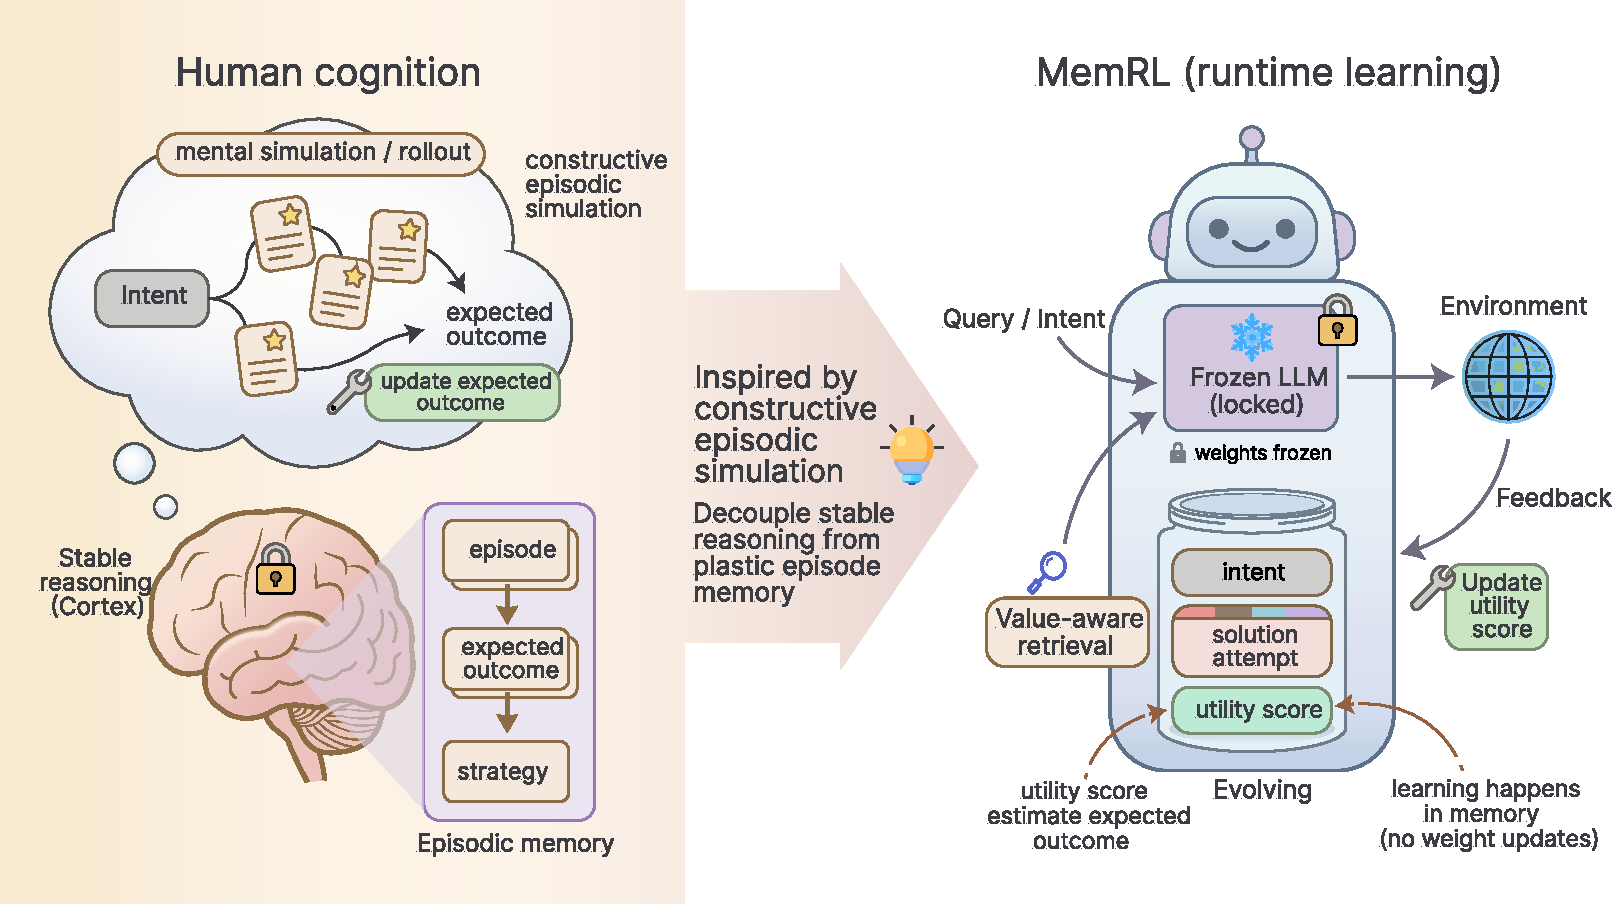
\includegraphics[width=\linewidth]{The_conceptual_framework_of_MemRL.pdf} 
    % \vspace{-10pt}
    \caption{The conceptual framework of MemRL.}
    \label{fig:memrl_framework}
    % \vspace{-10pt}
\end{figure}

This limitation underscores a critical research question: \textbf{How can we enable an agent to continuously improve its performance after deployment, without compromising the stability of its pre-trained backbone?} Our objective is to achieve an agent that evolves with continued usage and rapidly adapts to new tasks after deployment, referred to as Runtime Continuous Learning  \citep{javed2023online,silver2025era_of_experience,parisi2019continual,wu2024continuallearninglargelanguage}, all while keeping the backbone model frozen to prevent catastrophic forgetting \citep{finn2017model,wei2025evo}.
To address this challenge, inspired by the human cognitive mechanism of constructive simulation, we propose \textbf{\textsc{MemRL}}, an approach that facilitates self-evolving agents by explicitly decoupling the model’s stable cognitive reasoning from dynamic episodic memory. Figure~\ref{fig:memrl_framework} illustrates the conceptual framework of our proposed \textsc{MemRL}.
Drawing on tries-and-errors manner in Reinforcement Learning (RL) to estimate expected experience utilities  \citep{sutton2018reinforcement}, we formalize the interaction between the frozen LLM and external memory as a Markov Decision Process (MDP)  \citep{puterman2014markov}. Unlike traditional methods that optimize the backbone model, \textsc{MemRL} optimizes the policy of memory usage without tuning model weights. 

\textsc{MemRL} organizes memory into a structured \textbf{Intent-Experience-Utility} triplet. This structure transforms retrieval from a passive semantic match task into an active decision-making process: \textbf{Two-Phase Retrieval} selects experiences based on their learned Q-values, reflecting expected utility, rather than semantic similarity alone \citep{watkins1992q}; \textbf{Utility-Driven Update} refines these Q-values through environmental feedback, applying Monte Carlo style updates~\citep{metropolis1949monte}.
This closed-loop cycle enables the agent to distinguish high-value memories from similar noise, effectively learning from both success and failure without high computational cost or catastrophic forgetting risks associated with weight updates. As for experiments, we validate \textsc{MemRL} on four diverse benchmarks, including HLE, BigCodeBench, ALFWorld, and Lifelong Agent Bench. Our results demonstrate consistent superiority over baselines, achieving relative improvement in exploration-heavy environments. Our in-depth analysis reveals a strong correlation between learned utility and task success, further confirming \textsc{MemRL}’s effectiveness.

% 1. 此处待补充点实验结果描述
% 2. 下面的贡献待修正
In summary, our contributions are threefold:
\begin{itemize}
    % \item We formalize the interaction between LLM agents and external memory as an MDP, providing a theoretical foundation for applying RL to memory management.
    \item We propose a runtime learning framework using Model-Memory decoupling and Intent-Experience-Utility triplet to reconcile the stability-plasticity dilemma, enabling tuning-free agent learning.
    %y原文：We propose a runtime learning framework based on Model-Memory decoupling and the Intent-Experience-Utility triplet, which reconciles the stability-plasticity dilemma by enabling agents to learn without parameter updates.
    % \item We introduce the MemRL, a non-parametric reinforcement learning algorithm for Two-Phase Retrieval and Utility-Driven Memory Curation that enables agents to self-evolve by optimizing memory utility rather than model parameters, opening up a new dimension for improving the capabilities of intelligent agents.
    % \item We introduce \textsc{MemRL}, a non-parametric reinforcement learning algorithm that implements Two-Phase Retrieval and Utility-Driven Memory Curation. This allows agents to self-evolve by optimizing memory utility, establishing a new paradigm for enhancing agent capabilities.
\item We introduce \textsc{MemRL}, a non-parametric approach enabling agent self-evolution via Two-Phase Retrieval and Utility-Driven Update.
    % \item We conduct extensive evaluations and provide deep insights into \textsc{MemRL}’s working mechanism. We analyze how it ensures structural integrity in complex tasks and theoretically substantiate its stability via Bellman contraction, exploring how utility-driven updates minimize catastrophic forgetting while maximizing positive transfer.
    \item We conduct extensive evaluations and provide a rigorous analysis for \textsc{MemRL}’s stability, showing how it ensures task integrity and minimizes forgetting.
\end{itemize}

% limit: HLE-泛化性


\section{Related Works}
\paragraph{Runtime Learning}
% Runtime learning asks whether an agent can \emph{improve after deployment} by accumulating and leveraging experience from an ongoing stream of interactions and feedback, rather than relying solely on offline, human-curated data. This view is highlighted by the ``era of experience'' perspective, which argues that increasingly capable agents will learn predominantly from self-generated interaction data and grounded reward signals \citep{silver2025era_of_experience}. In our setting, runtime learning also comes with a practical constraint: the agent should keep improving under prolonged use and evolving tasks \emph{without} repeatedly updating the pretrained backbone, so as to preserve stable reasoning while avoiding the cost and instability of frequent online fine-tuning. This framing is related to, but distinct from, continual/lifelong learning and test-time adaptation: continual learning is typically studied under \emph{parametric} updates and focuses on the stability--plasticity dilemma and catastrophic forgetting \citep{parisi2019continual,wu2024continuallearninglargelanguage}, whereas test-time adaptation/training updates model parameters at inference time to cope with distribution shifts \citep{sun2020test,wang2020tent,liang2025comprehensive}. More recently, LLM-agent research increasingly places ``post-deployment learning'' in \emph{external state, memory, and policies}, and evaluates sustained learning and transfer via long-horizon benchmarks \citep{zheng2025lifelong,wei2025evo,zhou2025rulearena}. However, existing approaches often emphasize memory writing/organization, while leaving the \emph{selection problem} under-specified: \emph{which} experiences should be retrieved and reused under feedback, beyond similarity-based heuristics. From a cognitive-science lens, this gap aligns with \emph{value-aware episodic control}---episodic memory supports preferential replay/consolidation of salient episodes and utility-guided retrieval \citep{tulving1972episodic,mcclelland1995there}. Motivated by this view, we frame runtime learning as learning \emph{what is valuable to remember}: interaction feedback assigns utility/salience to episodes and uses it to guide retrieval and reuse (e.g., via selective replay), enabling sustained improvement with a fixed backbone \citep{schaul2015prioritized,pritzel2017neural}.
% Runtime Learning focuses on agent improvement post-deployment through interaction streams rather than offline data, a shift toward the ``era of experience" \citep{silver2025era_of_experience}. Unlike Continual Learning, which typically involves parametric updates and addresses catastrophic forgetting \citep{parisi2019continual,wu2024continuallearninglargelanguage}, or Test-Time Adaptation, which modifies parameters to handle distribution shifts \citep{sun2020test,wang2020tent,liang2025comprehensive}, our setting constrains the backbone to remain frozen to ensure stability and efficiency. While recent LLM-agent research utilizes external memory for post-deployment learning \citep{zheng2025lifelong,wei2025evo,zhou2025rulearena}, most works emphasize memory organization over the selection problem—identifying which experiences to reuse under feedback. Drawing from value-aware episodic control, where memory supports utility-guided retrieval \citep{tulving1972episodic,mcclelland1995there}, we frame runtime learning as identifying valuable episodes. By using interaction feedback to assign utility, our approach guides retrieval and reuse without weight modification, ensuring sustained improvement \citep{schaul2015prioritized,pritzel2017neural}.
Runtime Learning focuses on the post-deployment improvement of agents through interaction streams rather than offline data, marking a shift toward the ``era of experience'' \citep{silver2025era_of_experience}. Unlike Continual Learning \citep{parisi2019continual,wu2024continuallearninglargelanguage} or Test-Time Adaptation \citep{sun2020test,wang2020tent,liang2025comprehensive}, which typically update parameters to handle forgetting or distribution shifts, our setting constrains the backbone to remain frozen to ensure stability and efficiency. While recent memory-augmented agents \citep{zheng2025lifelong,wei2025evo,zhou2025rulearena} emphasize memory organization, the selection problem---identifying which experiences to reuse under feedback---remains a critical challenge. Drawing from value-aware episodic control \citep{tulving1972episodic,mcclelland1995there}, we frame runtime learning as identifying valuable episodes. By using interaction feedback to assign utility, our approach guides retrieval and reuse without weight modification, thereby ensuring sustained improvement \citep{pritzel2017neural}.
% Continual Learning studies how a model can acquire new knowledge over a sequence of tasks while preserving performance on previously learned ones. A central challenge is the stability--plasticity dilemma, which often manifests as catastrophic forgetting. Classical approaches include constraining drift of important parameters via regularization, maintaining behavioral consistency through distillation, and using explicit memory constraints or replay mechanisms to preserve coverage of past data distributions  \cite{kirkpatrick2017overcoming,li2017learning,lopez2017gradient}. However, these methods typically rely on repeated parameter updates or implicit modifications to the model, which are especially constrained in the context of large models and agentic systems: online updates are costly and slow, and weight changes can more easily perturb the boundaries of a model's original capabilities. Recent surveys on continual learning for LLMs further systematize these difficulties and emphasize the importance of external mechanisms and non-parametric pathways  \cite{wu2024continuallearninglargelanguage}. Therefore, from a continual learning perspective, if we aim for agents to improve with use while preserving the stability of the backbone, a more practical direction is to shift plasticity from the parameter space to external structures and controlled experience-update channels.

% T-T-train

% Continual learning addresses the stability-plasticity dilemma, aiming to acquire new knowledge sequentially without suffering from catastrophic forgetting. Classical approaches—such as regularization, distillation, and experience replay—mitigate forgetting by constraining parameter updates or preserving past data distributions  \citep{kirkpatrick2017overcoming,li2017learning,lopez2017gradient}. However, these parametric methods are computationally expensive for LLMs and risk destabilizing the pre-trained backbone through frequent online updates. Recent surveys on continual learning for LLMs further systematize these difficulties and emphasize the importance of external mechanisms and non-parametric pathways \citep{wu2024continuallearninglargelanguage}.  Therefore, from a continual learning perspective, if we aim for agents to improve with use while preserving the stability of the backbone, a more practical direction is to shift plasticity from the parameter space to external structures and controlled experience-update channels.


\paragraph{Reinforcement Learning}
% Reinforcement learning has been widely adopted for aligning LLMs and optimizing preferences. A representative paradigm is to construct reward signals from human feedback and optimize the model policy accordingly, shaping the output distribution  \cite{stiennon2020learning,ouyang2022training}. More recent preference optimization objectives improve training efficiency and stability, yet the learning target remains the model policy itself and still depends on parameter-level updates  \cite{rafailov2023direct,ethayarajh2024kto}. In parallel, agent-oriented research explores how interaction signals can improve tool use and action decision-making, and investigates mechanisms by which language models execute composite actions in environments  \cite{schick2023toolformer}. Despite the demonstrated effectiveness of reward-driven optimization, these methods generally place learning in the model parameters or additional trainable modules, and thus do not fundamentally avoid the cost of online updates or the risk of forgetting. More importantly, the main line of RL-for-LLMs focuses on optimizing model behavior, whereas it less frequently frames \emph{memory usage} as a learnable decision problem: treating memory retrieval as action selection and learning an iterative value function from environmental feedback, thereby enabling continual improvement with a frozen backbone. This gap directly motivates methods that apply reinforcement learning \emph{on memory}.

Reinforcement learning has been widely adopted for LLMs enhancement. A representative paradigm is to construct reward signals from human feedback and optimize the model policy accordingly to align with human preference  \citep{stiennon2020learning,ouyang2022training}. Other recent approaches leverage rule-based verifiers to improve LLMs' reasoning capabilities  \citep{guo2025deepseek,yu2025dapo}. In parallel, agent-oriented research explores how interaction signals can improve tool use and action decision-making, and investigates mechanisms by which language models execute composite actions in environments  \citep{schick2023toolformer}. Despite the demonstrated effectiveness of reward-driven optimization, these methods generally place learning in the model parameters or additional parametric modules, and thus do not avoid the cost of online updates or the risk of forgetting. In contrast, our method frames memory usage as a learnable decision problem and applies \emph{non-parametric} reinforcement learning on memory to bypass the risk.

\paragraph{Agentic Memory}
% To avoid frequent fine-tuning, external memory and retrieval augmentation have become central for improving agent capabilities. Retrieval-Augmented Generation (RAG) retrieves relevant external fragments and injects them into the context, introducing external knowledge and experience without modifying model parameters  \cite{lewis2020retrieval,karpukhin2020dense}. However, retrieval in RAG is often static and reactive, relying primarily on semantic similarity signals and lacking mechanisms to evaluate and continuously update the utility of memories. Building on this paradigm, agent memory systems further expand memory forms and management strategies. Reflection-based memory writes back successes and failures as reusable experiences  \cite{shinn2023reflexion}, and hierarchical memory scheduling alleviates context-window constraints through finer-grained read/write policies  \cite{packer2024memgptllmsoperatingsystems}. In 2025, agentic memory has accelerated toward more systematized designs. MemOS abstracts memory as a governable resource and emphasizes unified representation, organization, and lifecycle management  \cite{li2025memos}. A-MEM emphasizes networked linking and memory evolution to support experience organization and reuse over time  \cite{xu2025mem}. LiCoMemory and Task Memory Engine improve long-horizon consistency and robustness in multi-step tasks via lightweight structured indexing and task-structured memory, respectively  \cite{huang2025licomemory,ye2025task}. Meanwhile, adaptive memory augmentation and feedback-driven updates have become increasingly prominent. MemInsight improves retrievability and reuse efficiency of historical interactions via automated augmentation  \cite{salama2025meminsight}. Learn to Memorize organizes the memory lifecycle as an optimizable framework to learn better storage, retrieval, and update strategies  \cite{zhang2025learn}. RFM-RAG maintains a dynamic evidence pool, turning retrieval from stateless access into stateful knowledge management  \cite{li2025retrieval}. Alongside these advances, benchmarks in 2025 increasingly focus on key abilities under long-term interaction, including memory retrieval in incremental multi-turn settings, runtime learning, selective forgetting, and sustained gains from experience reuse  \cite{hu2025evaluating,wei2025evo,tan2025membench}.

% Despite these advances toward memory systems that can store, organize, and update, most methods still rely on similarity-driven signals and heuristic rules for retrieval decisions, or depend on relatively heavy training of additional learnable modules. They generally lack a memory-utility estimate that is strictly aligned with environmental returns and stably convergent under repeated exposure, making it difficult to consistently distinguish high-value experiences from redundant noise as similar tasks recur. Cognitive science on constructive episodic simulation emphasizes that humans form stable strategies through analogical transfer and repeated practice, and that memories undergo reconsolidation after retrieval, continuously re-evaluating their effectiveness under feedback  \cite{schacter2007constructive,gick1980analogical,nader2000fear}. Motivated by this gap and inspiration, we propose MemRL. With a frozen LLM backbone, MemRL organizes memory into an Intent--Experience--Utility structure and explicitly formulates memory selection as a decision process. It learns an iterative utility estimate (Q-value) from environmental feedback and leverages multi-epoch repeated exposure to stabilize value estimation, thereby advancing static similarity retrieval toward value-driven, self-evolving memory retrieval and updating.


\begin{figure*}[h]
    \centering
    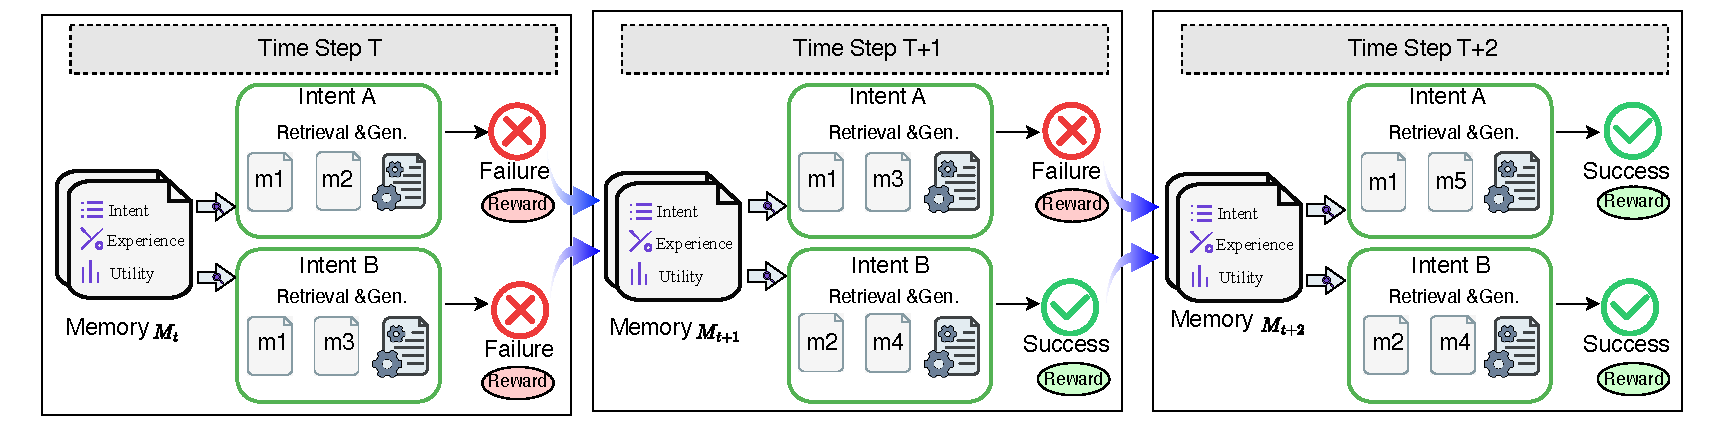
\includegraphics[width=\linewidth]{mdp.pdf}
    \caption{
    An illustrative example of memory-augmented decision making under a Markov Decision Process.
    At time step $t$, the agent starts with an initial memory set $\mathcal{M}_t$.
    At time step $t{+}1$, an intent (\textit{Intent A}) retrieves relevant past experiences, but initially leads to a failed generation.
    In contrast, another intent (\textit{Intent B}) succeeds, and its associated experience is added to memory.
    At time step $t{+}2$, \textit{Intent A} retrieves the newly stored successful experience from \textit{Intent B}, resulting in a successful outcome.
    This example shows how memory retrieval enables knowledge reuse across intents, implicitly supporting self-evolution through shared experiences.
    }
    \label{fig:mmdp}
\end{figure*}


To avoid the costs of fine-tuning, external memory systems have evolved from a static RAG paradigm to dynamic, governable memory structures  \citep{lewis2020retrieval,karpukhin2020dense}. Early agentic memory introduced reflection mechanisms and hierarchical management to handle long context experiences \citep{shinn2023reflexion,packer2024memgptllmsoperatingsystems}. More recent frameworks have systematized the memory lifecycle, focusing on unified storage and structured indexing for complex tasks  \citep{li2025memos,xu2025mem,huang2025licomemory,ye2025task}. Furthermore, adaptive approaches now explore improving retrieval via feedback-driven updates or automated augmentation  \citep{salama2025meminsight,zhang2025learn,li2025retrieval,zhou2025memento}. However, except for training additional learnable modules, most existing methods still rely predominantly on semantic similarity or heuristic rules, lacking a rigorous metric to evaluate the actual utility of a memory in maximizing returns. Inspired by cognitive theories of memory reconsolidation  \citep{schacter2007constructive,gick1980analogical,nader2000fear}, \textsc{MemRL} bridges this gap by formulating retrieval as a value-based decision process, learning robust utility estimates (Q-values) from environmental rewards to distinguish high-value experiences.


\section{Problem Formulation}
\label{sec:problem}

In this section, we formally define the problem of memory-augmented generation and establish the theoretical link between agent policy and memory retrieval. We adopt the formulation of Memory-Based Markov Decision Process (M-MDP)  \citep{zhou2025memento}, and apply our non-parametric reinforcement learning approach to it.
Figure~\ref{fig:mmdp} provides an illustrative example of this memory-augmented decision process, showing how retrieval outcomes and memory evolution unfold over multiple time steps.


% \subsection{Memory-Augmented Agent Policy}

% To enable the agent to self-evolve, we inherit the M-MDP as the problem formulation  \citep{zhou2025memento}. The M-MDP is formally defined as a tuple $\langle \mathcal{S}, \mathcal{A}, \mathcal{P}, \mathcal{R}, \gamma, \mathcal{M} \rangle$, where $\mathcal{S}$ denotes the state space, $\mathcal{A}$ the action space, $\mathcal{P}:\mathcal{S}\times\mathcal{A}\rightarrow\mathbb{R}$ the transition dynamics, $\mathcal{R}:\mathcal{S}\times\mathcal{A}\rightarrow\mathbb{R}$ the reward function, $\gamma \in [0,1)$ the discount factor, and $\mathcal{M}=(\mathcal{S}\times\mathcal{A}\times\mathbb{R})^{*}$ the evolving memory space containing past experiences \citep{zhou2025memento}.
% In this setting, the policy $\pi$ not only generates tokens but first selects a memory context $m$ based on a retrieval distribution $\mu(\cdot | s, \mathcal{M})$, allowing the agent to leverage historical data for better performance in downstream tasks.

% We consider a generalist agent interacting with an environment or user over discrete time steps. At each step $t$, the agent receives a state $s_t$, e.g., a user query or task description, and has access to an external memory bank $\mathcal{M}$. The agent's objective is to generate a response $y_t$ that maximizes a reward signal.
% Following this formulation, the behavior of a memory-augmented agent can be decomposed into two distinct phases: \textit{Retrieve} and \textit{Generation}. The joint policy $\pi(y_t| s_t, \mathcal{M}_t)$ is defined as the marginal probability over all possible retrieved memory items \citep{zhou2025memento}:
% \begin{equation}
% \label{eq:policy_decomp}
% \pi(y_t |  s_t, \mathcal{M}_t) = \sum_{m \in \mathcal{M}_t} \underbrace{\mu(m |  s_t, \mathcal{M}_t)}_{\text{Retrieval Policy}} \cdot \underbrace{p_{\text{LLM}}(y_t |  s_t, m)}_{\text{Inference Policy}}
% \end{equation}
% where:
% \begin{itemize}
% \item $\mu(m |  s_t, \mathcal{M}_t)$ represents the \textbf{Retrieval Policy}, which assigns a probability to selecting a specific memory context $m$ composed of past intents and experiences. from the memory bank $\mathcal{M}_t$ given the current state $s_t$.
% \item $p_{\text{LLM}}(y_t |  s_t, m)$ represents the \textbf{Inference Policy}, typically parameterized by a frozen LLM. It models the likelihood of generating output $y_t$ conditioned on both the query $s_t$ and the retrieved context $m$.
% \end{itemize}

\subsection{Memory-Augmented Agent Policy}
\label{sec:mmdp}
To enable the agent to self-evolution, we adopt the M-MDP framework \citep{zhou2025memento}, defined by the tuple $(\mathcal{S}, \mathcal{A}, P, \mathcal{R}, \gamma, \mathcal{M})$. Here, $\mathcal{S}$ and $\mathcal{A}$ represent state and action spaces, $P$ is the transition dynamics, $\mathcal{R}$ is the reward function of state and action, $\gamma \in [0,1)$ denotes the discount factor, and $\mathcal{M} = (\mathcal{S} \times \mathcal{A} \times \mathbb{R})^*$ constitutes the evolving memory bank of past experiences \citep{zhou2025memento}. At each step $t$, the agent receives state $s_t$ and leverages $\mathcal{M}_t$ to generate a response $a_t$ maximizing the expected reward. The joint policy $\pi(a_t | s_t, \mathcal{M}_t)$ is formulated as the marginal probability over all possible retrieved items $m$ \citep{zhou2025memento}:
\begin{equation}
\pi(a_t | s_t, \mathcal{M}_t) = \sum_{m \in \mathcal{M}_t} \mu(m | s_t, \mathcal{M}_t) p_{LLM}(a_t | s_t, m) \label{eq:joint_policy}.
\end{equation}
where $\mu(m | s_t, \mathcal{M}_t)$ is the \textbf{Retrieval Policy} for selecting memory contexts, and $p_{LLM}(a_t | s_t, m)$ is the \textbf{Inference Policy} parameterized by a frozen LLM. This approach transforms retrieval from a passive match into an active decision process, effectively accounting for the functional \emph{utility} of $m$ in generating successful outcomes $a_t$.

% 下面这段话需要斟酌下是否要把RAG和Memory retrival类方法分开来讨论
In previous RAG or memory-based agentic paradigms, the retrieval policy $\mu$ is usually determined by a fixed vector similarity metric, e.g., cosine similarity of embeddings. While effective for semantic matching, such policies fail to account for the \textit{utility} of a memory, i.e., whether retrieving $m$ actually leads to a successful outcome $a_t$.

% \subsection{Memory-Augmented Agent Policy}
% To enable the agent to self-evolution, we adopt the M-MDP framework \citep{zhou2025memento}, defined by the tuple $(\mathcal{S}, \mathcal{A}, P, \mathcal{R}, \gamma, \mathcal{M})$. Here, $\mathcal{S}$ and $\mathcal{A}$ represent state and action spaces, $P$ is the transition dynamics, $\mathcal{R}$ is the reward function, $\gamma \in [0,1)$ denotes the discount factor, and $\mathcal{M} = (\mathcal{S} \times \mathcal{A} \times \mathbb{R})^*$ constitutes the evolving memory bank of past experiences \citep{zhou2025memento}. At each step $t$, the agent receives state $s_t$ and leverages $\mathcal{M}_t$ to generate a response $y_t$ maximizing the expected reward. The joint policy $\pi(y_t | s_t, \mathcal{M}_t)$ is formulated as the marginal probability over all possible retrieved items $m$ \citep{zhou2025memento}:
% \begin{equation}
% \pi(y_t | s_t, \mathcal{M}_t) = \sum_{m \in \mathcal{M}_t} \mu(m | s_t, \mathcal{M}_t) p_{LLM}(y_t | s_t, m) \label{eq:joint_policy}.
% \end{equation}
% where $\mu(m | s_t, \mathcal{M}_t)$ is the \textbf{Retrieval Policy} for selecting memory contexts, and $p_{LLM}(y_t | s_t, m)$ is the \textbf{Inference Policy} parameterized by a frozen LLM. This approach transforms retrieval from a passive match into an active decision process, effectively accounting for the functional \emph{utility} of $m$ in generating successful outcomes $y_t$.

% % 下面这段话需要斟酌下是否要把RAG和Memory retrival类方法分开来讨论
% In previous RAG or memory-based agentic paradigms, the retrieval policy $\mu$ is usually determined by a fixed vector similarity metric, e.g., cosine similarity of embeddings. While effective for semantic matching, such policies fail to account for the \textit{utility} of a memory, i.e., whether retrieving $m$ actually leads to a successful outcome $y_t$.

% \subsection{Non-Parametric Reinforcement Learning on Memory}

% We bridge this theoretical formulation to our proposed method, MemRL, by mapping the abstract components of M-MDP to our specific \textbf{Intent-Experience-Utility} triplet structure respectively:

% \paragraph{Intent as State.}
% In our formulation, we instantiate $s_t\in\mathcal{S}$ as the user intent, encapsulated by the embedding vector of the current query or task description  \cite{lewis2020retrieval}. We utilize these semantic vectors to retrieve similar intents, forming the basis for state generalization.

% \paragraph{Experience Selection as Action.}
% We redefine the action $a_t\in\mathcal{A}$ in M-MDP as the selection of a specific memory block, i.e., experience. Specifically, the action space is dynamic and discrete, corresponding to the current set of available experiences in memory, i.e., $\mathcal{A}_t = \mathcal{M}_t$. Choosing an action $a_t = m$ implies retrieving the specific experience $m$, e.g., a successful past trajectory or failure decision with reflections, to augment the frozen LLM generator  \cite{zhou2025memento}.

% \paragraph{Q-Value as Utility.}
% The core of our non-parametric approach lies in the evaluation of these actions. We map the state-action value function $Q(s, a)$ to the utility of an experience. $Q(s, m)$ quantifies the expected benefit of applying experience $m$ for intent $s$, distinguishing high-quality strategies from irrelevant noise. The goal of MemRL is to learn an optimal retrieval policy $\mu^*$ that selects the experience with the highest expected utility:
% \begin{equation}
% \label{eq:optimal_retrieval}
% \mu^*(m | s, \mathcal{M}) = {\arg\max}_{m \in \mathcal{M}} Q(s, m)
% \end{equation}

% \paragraph{Non-Parametric Learning.}
% Unlike parametric methods that approximate $Q(s, a)$ via fine-tuning the LLMs or introducing an extra neural network  \cite{zhou2025memento, zhang2025learn}, we maintain and update these utility values directly within the Intent-Experience-Utility triplet in a non-parametric fashion. The fitting process is driven by the environmental reward $r_t$ received after task completion, e.g., user feedback or execution success. Following the Bellman backup, the utility of a candidate experience is updated to minimize the discrepancy between the expected and actual outcome  \cite{bellman1966dynamic,sutton2018reinforcement}:
% \begin{equation}
% Q(s, m) \leftarrow Q(s, m) + \alpha \cdot (r_t - Q(s, m))
% \end{equation}
% where $\alpha$ is the learning rate. This mechanism ensures that the \textit{Utility} in our triplet structure dynamically converges to the true value of the experience, enabling the retrieval policy $\mu$ to evolve towards optimality without altering the LLM's parameters.

% \subsection{Non-Parametric Reinforcement Learning}
% To overcome the limitations of static similarity-based retrieval, we operationalize the M-MDP framework by formulating memory retrieval as a value-based decision-making process. Unlike parametric approaches that optimize $\pi_{\text{LLM}}$ via weight updates, we aim to optimize the retrieval policy $\mu(m| s, \mathcal{M})$ directly within the memory space. We map the abstract M-MDP components to a specific Intent-Experience-Utility structure:

% \textbf{From Semantic Matching to Decision Making.} We instantiate the state $s$ as the User Intent, encapsulated by the embedding of the current query  \citep{lewis2020retrieval}. Consequently, the action space $\mathcal{A}_t$ becomes dynamic and discrete, corresponding to the selection of a specific $m$ from the current memory bank $\mathcal{M}_t$. Under this formulation, retrieving from memory is no longer a passive matching task but an active action $a_t=m$ taken to augment the generator  \citep{zhou2025memento}.

% \textbf{Defining Utility via Q-Values.} The core of our framework is the shift from estimating semantic relevance to estimating functional utility. We define the state-action value function $Q(s, m)$ as the expected utility of applying the retrieved context $m$ for intents similar to $s$. The objective of \textsc{MemRL} is to learn an optimal retrieval policy $\mu^*$ that selects context maximizing this expected utility:
% \begin{equation}
%     \mu^*(m| s, \mathcal{M}) = \arg\max_{m \in \mathcal{M}} Q(s, m)
% \end{equation}
% This $Q$-value serves as a critic, distinguishing high-value strategies from irrelevant noise that may share high semantic similarity.

% \textbf{Non-Parametric Learning.} Since the action space of the retrieval policy $\mu$ in our setting is decoupled from the LLMs' generation space, we can perform learning without modifying the LLMs' weights. Upon receiving an environmental feedback $r$, e.g., execution success, we can update the Q-value of the retrieved memory context using a Temporal-Difference (TD) error \citep{sutton1988learning}:
% \begin{equation}
% \label{equ:bellman-q}
%     % Q(s, m) \leftarrow Q(s, m) + \alpha \cdot (r_t - Q(s, m))
%     Q(s,m) \leftarrow Q(s,m) + \alpha [r + \gamma \max Q(s',m') - Q(s,m)]
% \end{equation}
% where $\alpha$ is the learning rate. This Bellman-style backup allows the utility estimates to converge to the true expected returns over time  \citep{bellman1966dynamic}. By maintaining and updating these Q-values explicitly within the memory structure, \textsc{MemRL} provides a non-parametric learning manner with a theoretical guarantee that enables the agent to self-evolve its capabilities through interaction.
\begin{figure*}[h]
    \centering
    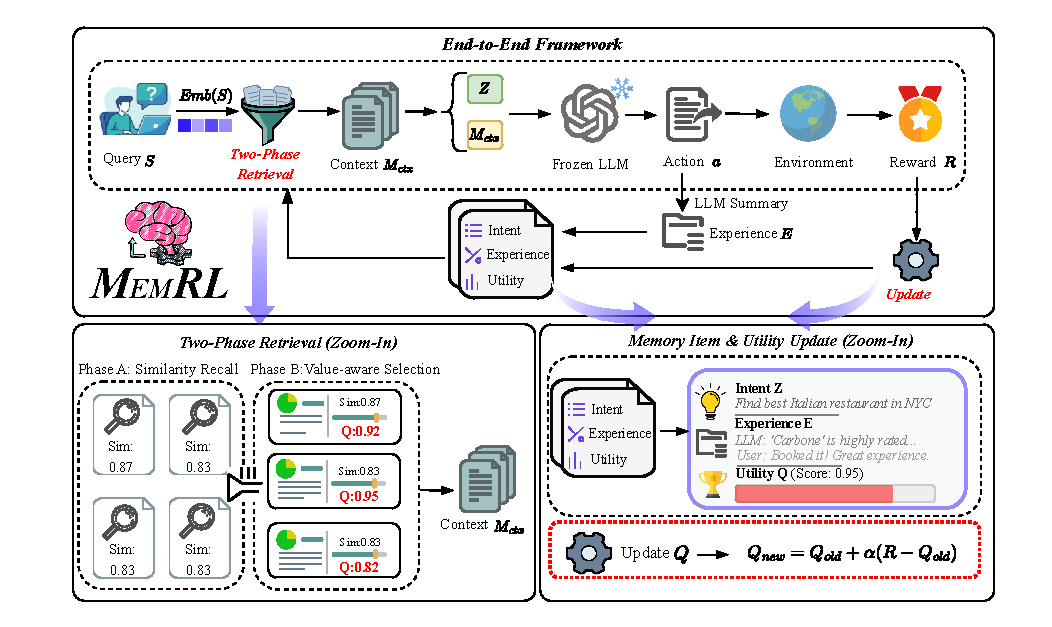
\includegraphics[width=\textwidth]{framework_overview.pdf} % 确保文件名正确
    
    % --- 修复重点：注意最后那个关闭的大括号 } ---
    \caption{\textbf{Overview of \textsc{MemRL}.} 
    \textbf{The end-to-end learning loop(Top)}: given a query $\mathbf{s}$, the agent retrieves context $\mathbf{m}_{ctx}$ from memory $\mathbf{M}$, generates output $\mathbf{y}$, and updates memory value $Q$ based on reward $R$.
    \textbf{Two-Phase Retrieval(Bottom Left)}: Candidates are recalled via similarity, then re-ranked using learned Q-values.
    \textbf{Utility Update(Bottom Right)}: Values ($Q$) are updated using environmental rewards to distinguish functional utility from semantic similarity.} 
    % -------------------------------------------
    
    \label{fig:framework}
\end{figure*}

\subsection{Non-Parametric Reinforcement Learning}
To overcome static similarity limitations, we operationalize the M-MDP framework by formulating memory retrieval as a value-based decision-making process \citep{zhou2025memento}. Unlike parametric methods optimizing $\pi_{LLM}$ via weight updates, we optimize the retrieval policy $\mu(m|s, \mathcal{M})$ directly within the memory space by mapping M-MDP components to a structured \textit{Intent-Experience-Utility} triplet:

\textbf{From Semantic Matching to Decision Making.} We instantiate state $s$ as the User Intent, encapsulated by the current query embedding \citep{lewis2020retrieval}. Consequently, the action space $\mathcal{A}_t$ becomes dynamic and discrete, corresponding to selecting a specific $m$ from the memory bank $\mathcal{M}_t$ \citep{zhou2025memento}. In this formulation, retrieval is not a passive matching task but a strategic decision step taken to augment the generator's action $a$~\citep{zhou2025memento}.


\textbf{Defining Utility via Q-Values.} While the agent's executable action $a$ is generated by the policy $\pi$ (as formalized in Sec.~\ref{sec:mmdp}), the quality of this generation is strictly conditioned on the retrieved context. Therefore, we adapt the traditional value function $Q(s, a)$ to the retrieval phase, defining $Q(s, m)$ as the expected utility of the subsequent action $a$ augmented by memory $m$. \textsc{MemRL} learns an optimal retrieval policy $\mu^*$ that maximizes this utility:
\begin{equation}
    \mu^*(m| s, \mathcal{M}) = \arg\max_{m \in \mathcal{M}} Q(s, m). \label{equ:optimal-policy}
\end{equation}
In this view, the Q-value acts as a critic for the retrieval mechanism, distinguishing memories that strategically aid the generator from irrelevant noise that merely shares high semantic similarity.


% \textbf{Defining Utility via Q-Values.} We shift from estimating semantic relevance to functional utility by defining the state-action value function $Q(s, m)$ as the expected utility of applying the retrieved context $m$ for intents similar to $s$. \textsc{MemRL} learns an optimal retrieval policy $\mu^*$ that maximizes this expected utility:
% \begin{equation}
%     \mu^*(m| s, \mathcal{M}) = \arg\max_{m \in \mathcal{M}} Q(s, m). \label{equ:optimal-policy}
% \end{equation}
% This Q-value acts as a critic, distinguishing high-value strategies from irrelevant noise that share high semantic similarity.

\textbf{Non-Parametric Learning.} Since the retrieval action space is decoupled from LLM generation, we perform learning without modifying model weights. Upon receiving environmental feedback $r$, we update the Q-value via a Temporal-Difference (TD) error \citep{sutton1988learning}:
\begin{equation}
\label{equ:bellman-q}
    Q(s,m) \leftarrow Q(s,m) + \alpha [r + \gamma \max Q(s',m') - Q(s,m)],
\end{equation}
or Monte Carlo style rule \citep{metropolis1949monte}:
\begin{equation}
\label{eq:q_update}
Q_{\text{new}} \leftarrow Q_{\text{old}} + \alpha \big(r - Q_{\text{old}}\big),
\end{equation}
where $\alpha$ is the learning rate. Equation~\ref{eq:q_update} performs as a naturally simplified version of Equation~\ref{equ:bellman-q} by setting $s'$ as a terminal state to balance complexity and performance, sharing a similar one-step MDP formulation with \citet{guo2025deepseek}. These manners allow utility estimates to converge to true expected returns over time \citep{bellman1966dynamic}. By explicitly updating Q-values within the memory structure, \textsc{MemRL} provides a non-parametric learning manner with a theoretical guarantee, enabling agents to self-evolve through interaction.

\section{\textsc{MemRL}}
% 具体的方法与实现细节，并要讨论好我们的方法跟认知科学的联系
\label{sec:method}

% MemRL aims to endow an agent with \textit{runtime self-evolving} capabilities while keeping the backbone LLM frozen. In contrast to fine-tuning-based paradigms that internalize experience by updating model parameters, MemRL learns \textit{how to use memory}---i.e., it optimizes the retrieval policy over an evolving external memory space.\textbf{The overall framework is illustrated in Figure~\ref{fig:framework}.}  Concretely, we (i) represent memory as a structured \textbf{Intent--Experience--Utility} triplet, (ii) perform \textbf{two-phase retrieval} that separates \textit{semantic recall} from \textit{utility-based selection}, and (iii) leverage \textbf{multi-epoch rehearsal} so that learned Q-values become reliable estimates of memory utility under repeated exposure, analogous to how humans acquire robust skills through repeated practice and memory reconsolidation.

Building upon the M-MDP formulation defined in Section~\ref{sec:problem}, we propose \textsc{MemRL}, a framework that enables frozen LLMs to self-evolve via non-parametric reinforcement learning. Instead of modifying the model weights $\theta$, \textsc{MemRL} optimizes the \textbf{retrieval policy} $\mu(m| s, \mathcal{M})$ within an evolving memory space. As illustrated in Figure~\ref{fig:framework}, the framework consists of three core components: (i) a structured \textbf{Intent-Experience-Utility} memory bank, (ii) a \textbf{Two-Phase Retrieval} mechanism that decouples semantic recall from value-aware selection, and (iii) a \textbf{Runtime Utility Update} rule that stabilizes Q-value estimation.

% \subsection{Similar is Not Always Useful}
% \label{subsec:objective}

% As formalized in Sec.~\ref{sec:prelim}, a memory-augmented agent decomposes behavior into \textit{Retrieve} and \textit{Generation} (Eq.~\ref{eq:policy_decomp}), where the retrieval policy $\mu(m | s, \mathcal{M})$ selects a memory context and the frozen inference policy $p_{\text{LLM}}(y| s,m)$ generates the response. Standard RAG or memory-based agent instantiates $\mu$ as a static nearest-neighbor rule in embedding space, implicitly assuming that \textit{semantic similarity implies utility}. However, in agentic settings, semantically similar experiences can be redundant or even harmful: retrieved trajectories may encode brittle tool-use routines (e.g., hard-coded API fields or web selectors) that break under minor interface shifts, and top-ranked similarity passages are not guaranteed to improve downstream generation  \cite{singh2025agentic,Cuconasu_2024,gan2024similarity}. Directly injecting such memory into the LLM context may introduce noise and harm performance. Therefore, MemRL explicitly separates \textbf{type-consistent recall} from \textbf{value-consistent selection}: it first recalls a semantically coherent candidate set of experiences, and then selects the final memory context according to utilities (Q-values) learned from environmental feedback.

\subsection{The Intent-Experience-Utility Triplet}
\label{subsec:memory_repr}

% We maintain an external memory bank as a set of triplets:
% \begin{equation}
% \mathcal{M}=\{(z_i, e_i, Q_i)\}_{i=1}^{|\mathcal{M}|},
% \end{equation}
% where $z_i$ denotes the embedding of the corresponding \textbf{Intent}, e.g., user query or task description, $e_i$ denotes the stored \textbf{Experience}, e.g., past solutions or trajectories, and $Q_i \equiv Q(z_i, e_i)$ denotes the expected \textbf{Utility} of applying that experience $e_i$ under intents similar to $z_i$.

% Given a task/query $s$, we compute its intent embedding $z(s)$ and define semantic similarity by cosine distance:
% \begin{equation}
% \mathrm{sim}(s, z_i) \triangleq \cos(z(s), z_i).
% \end{equation}
% In addition to retrieval based on semantic similarity, we also have a value-aware selection process. After two-phase retrieval, the final retrieved memory context is a subset $\mathcal{M}_{\text{ctx}}(s)\subseteq \mathcal{M}$, which is injected into the frozen LLM for generation:
% \begin{equation}
% y \sim p_{\text{LLM}}(y | s, \mathcal{M}_{\text{ctx}}(s)).
% \end{equation}

To support value-based decision-making, we structure the external memory $\mathcal{M}$ not merely as key-value pairs, but as a set of triplets:
\begin{equation}
\mathcal{M}=\{(z_i, e_i, Q_i)\}_{i=1}^{|\mathcal{M}|},
\end{equation}
where $z_i$ represents the \textbf{Intent}, $e_i$ stores the raw \textbf{Experience} (e.g., a successful solution trace or trajectory), and $Q_i$ denotes the learned \textbf{Utility}. $Q_i$ approximates the expected return of applying experience $e_i$ to intents similar to $z_i$, serving as the \textit{critic} in RL.

% \subsection{Two-Phase Retrieval: From Semantic Recall to Value-Aware Selection}
% \label{subsec:two_phase}

% % MemRL implements retrieval via two consecutive phases: \textbf{Phase-A} performs semantic recall to obtain a candidate pool of type-consistent experiences, while \textbf{Phase-B} performs value-aware selection to determine which memories are actually injected into the LLM context.

% Standard RAG or memory systems rely solely on semantic similarity, implicitly assuming that ``similar implies useful.'' However, in agentic tasks, semantically relevant contexts may encode brittle, environment-specific routines that fail to generalize  \citep{singh2025agentic,Cuconasu_2024,gan2024similarity,zhou2024trad}. To address this, \textsc{MemRL} implements a Two-Phase Retrieval strategy that filters candidates first by relevance, then by utility.

% \paragraph{Phase A: Similarity-Based Recall.}\label{phaseA}Given a current query state $s$, we first isolate a candidate pool $\mathcal{C}(s)$ of semantically consistent experiences to ensure the retrieval is contextually relevant. We compute the cosine similarity $sim(s, z_i)$ and filter the memory bank:
% \begin{equation}
% \label{eq:phase a}
% \mathcal{C}(s) = \text{TopK}_{k_1}(\{i | sim(s, z_i) > \delta\}, \text{by } sim)
% \end{equation}
% where $\delta$ is a sparsity threshold. This phase acts as a coarse filter, reducing the search space from the entire memory $\mathcal{M}$ to a relevant subset $\mathcal{C}(s)$. Notably, if $\mathcal{C}(s)=\emptyset$, \textsc{MemRL} injects no memory and relies solely on the frozen LLM for broader exploration.

% \paragraph{Phase B: Value-Aware Selection.}To select the optimal context from $\mathcal{C}(s)$, we incorporate the learned utility $Q$. We define a composite scoring function that balances exploration (via semantic matching) and exploitation (via high-utility history):
% \begin{equation}
% \label{eq:score}
% \text{score}(s, z_i, e_i) = (1-\lambda) \cdot \hat{sim}(s, z_i) + \lambda \cdot \hat{Q}(z_i, e_i)
% \end{equation}
% where $\hat{\cdot}$ denotes z-score normalization within the candidate pool, and $\lambda \in [0, 1]$ modulates the trade-off. As $\lambda \rightarrow 1$, the policy prioritizes proven utility; as $\lambda \rightarrow 0$, it reverts to standard similarity-based retrieval. The final context $\mathcal{M}_{ctx}(s)$ consists of the top-$k_2$ items maximizing this score:
% \begin{equation}
% \mathcal{M}_{ctx}(s) = \text{TopK}_{k_2}(\mathcal{C}(s), \text{by } \text{score}).
% \end{equation}
% This mechanism effectively filters out ``distractor'' memories—those that are semantically similar but historically yielded low returns (low Q-values). We further validate the necessity of normalization and similarity threshold in Section \ref{sec:stable in mem rl exp}, demonstrating that z-score normalization and strict similarity threshold are essential for filtering noise and maintaining low forgetting rates during self-evolution.  
\subsection{From Semantic Recall to Value-Aware Selection}
\label{subsec:two_phase}
Standard RAG systems assume ``similar implies useful,'' but agentic tasks often involve environment-specific routines that generalize poorly \citep{singh2025agentic,Cuconasu_2024,gan2024similarity,zhou2024trad}. Therefore, \textsc{MemRL} implements a \textbf{Two-Phase Retrieval} strategy. 
\textbf{Phase A: Similarity-Based Recall.} Given query $s$, we isolate a candidate pool $\mathcal{C}(s)$ of semantically consistent experiences by filtering memory bank $\mathcal{M}$ via cosine similarity and a sparsity threshold $\delta$:
\begin{equation}
\label{eq:phase a}
\mathcal{C}(s) = \text{TopK}_{k_1}(\{i | sim(Emb(s), Emb(z_i)) > \delta\}),
\end{equation}
where $Emb$ represents the Embedding Model to transfer the raw text to a vector.
If $\mathcal{C}(s)=\emptyset$, \textsc{MemRL} relies solely on the frozen LLM for exploration. 
\textbf{Phase B: Value-Aware Selection.} To determine the final context $\mathcal{M}_{ctx}(s)$, we select top-$k_2$ items from $\mathcal{C}(s)$ using a composite score balancing exploration (similarity) and exploitation (utility $Q$):
\begin{equation}
\label{eq:score}
% \begin{aligned}
\text{score}(s, z_i, e_i) = (1-\lambda) \cdot \hat{sim}(Emb(s), Emb(z_i)) + \lambda \cdot \hat{Q_i}.
% \end{aligned}
\end{equation}
where $\hat{\cdot}$ denotes z-score normalization and $\lambda \in [0, 1]$ modulates the trade-off. This mechanism filters out ``distractor'' memories—those semantically similar but with low historical utility. As detailed in Section~\ref{sec:stable in mem rl exp}, normalization and strict similarity thresholds are essential for noise filtering and maintaining stability during self-evolution.


% \subsubsection{Similarity-Based Recall}
% \label{subsubsec:phaseA}

% \textbf{Input:} an intent $s$ and the full memory bank $\mathcal{M}$. \quad
% \textbf{Output:} a semantically coherent candidate set (or lists) used for Phase-B ranking.

% We first filter memory items by a similarity threshold $\tau$:
% \begin{equation}
% \mathcal{C}(s)=\{i \in \{1,\dots,|\mathcal{M}|\} | \mathrm{sim}(s,z_i)\ge \tau\}.
% \end{equation}
% Equivalently, $\tau$ can be chosen to keep approximately the top-$n\%$ most similar items. Notably, if $\mathcal{C}(s)=\emptyset$, MemRL injects no memory and relies solely on the frozen LLM for better exploration, i.e., $\mathcal{M}_{\text{ctx}}(s)=\emptyset$. Otherwise, we then cap the candidate pool by selecting at most $k_1$ items ranked by similarity:
% \begin{equation}
% \tilde{\mathcal{C}}(s)=\mathrm{TopK}_{k_1}\big(\mathcal{C}(s), \mathrm{sim}(s,\cdot)\big),
% \end{equation}
% where $|\tilde{\mathcal{C}}(s)|\le k_1$ due to thresholding.

% \paragraph{Multi-epoch grouping.}
% In practice, similar tasks might be encountered multiple times as time goes by. Thus, Phase-A can further organize $\tilde{\mathcal{C}}(s)$ into $|\tilde{\mathcal{C}}(s)|$ lists $\{\mathcal{L}_1,\dots,\mathcal{L}_{|\tilde{\mathcal{C}}(s)|}\}$ by task/intent cluster, where each list contains one intent and multiple experiences accumulated over multiple tries. Importantly, Phase-A candidates are \textit{not} directly injected into the LLMs; they serve only as the search space for Phase-B value-aware selection.

% \subsubsection{Value-Aware Selection}
% \label{subsubsec:phaseB}

% \textbf{Input:} $n$ lists $\{\mathcal{L}_1,\dots,\mathcal{L}_n\}$ (or the flat candidate set). \quad
% \textbf{Output:} the final injected context $\mathcal{M}_{\text{ctx}}(s)$.

% We first flatten the lists into a candidate pool:
% \begin{equation}
% \mathcal{P}(s)=\bigcup_{j=1}^{n}\mathcal{L}_j.
% \end{equation}
% Then we normalize similarity scores and utilities within $\mathcal{P}(s)$ using z-score normalization and obtain $\widehat{\mathrm{sim}}(s,z)$ and $\widehat{Q}(z,e)$.
% We then define the final selection score as a convex combination:
% \begin{equation}
% \label{eq:value_score}
% \mathrm{score}(s,z,e)=\lambda \cdot \widehat{\mathrm{sim}}(s,z) + (1-\lambda)\cdot \widehat{Q}(z,e),
% \end{equation}
% where $\lambda \in [0,1]$. The weights $\lambda$ control the trade-off between semantic relevance and expected utility: as $\lambda \rightarrow 0$, MemRL approaches pure utility-based retrieval; as $\lambda\rightarrow 1$, it reduces to similarity-only retrieval.

% Finally, we rank candidates by $\mathrm{score}(s,z,e)$ and select at most $k_2$ memory contexts to form the injected context:
% \begin{equation}
% \label{eq:final_ctx}
% \mathcal{M}_{\text{ctx}}(s)=\mathrm{TopK}_{k_2}\big(\mathcal{P}(s), \mathrm{score}(s,\cdot)\big).
% \end{equation}



% \subsection{Multi-Epoch Rehearsal: Stabilizing Utility Estimation}
% \label{subsec:rehearsal}

% A central requirement of MemRL is that the learned Q-value should reflect the true expected benefit of referring experience $e$ under intent $s$, rather than an accidental outcome from a single trial. In human cognition, robust skill acquisition typically requires repeated exposure and practice; retrieved memories are strengthened or weakened through repeated rehearsal and feedback-driven reconsolidation. Inspired by this, MemRL performs \emph{runtime value propagation} over episodic memory under repeated exposure to the same task family. After each interaction, the agent retrieves candidate memories, executes the task, observes a reward signal, and applies a Bellman-style backup to update the corresponding utility estimates. Repeating this backup across successive episodes reduces the variance of sparse and noisy rewards, driving the Q-values toward stable estimates and enabling reliable Two-Phase Retrieval.
\subsection{Non-Parametric RL on Memory}
% \subsection{Utility-Driven Update: Non-Parametric RL on Memory}
\label{subsec:update}

The core of \textsc{MemRL} is the continuous refinement of Q-values based on environmental feedback, enabling the agent to ``remember'' what works. During runtime, \textsc{MemRL} performs learning entirely in memory space. With the retrieved context $m$, the agent samples an action $a$ according to the policy $\pi$ defined in Eq.~\ref{eq:joint_policy}. Executing $a$ then yields an environmental reward $r$ (e.g., execution success or scalar score). For the memories actually injected into the input context $\mathcal{M}_{\text{ctx}}(s)$, we update their utilities in triplets with a Monte Carlo style rule, i.e., the Eq.~\ref{eq:q_update}, following the runtime learning loop shown in Figure~\ref{fig:framework}. 
This update drives $Q_{\text{new}}$ toward the empirical expected return of using experience $e_i$ under similar intents. Meanwhile, for each sampled trajectory, we use an LLM to summarize the experience~\citep{fang2025memp}, and write it back into the memory bank as a new triplet $(z, e_{\text{new}}, Q_{\text{init}})$, enabling continual expansion of experience while keeping the LLM parameters unchanged.

% \subsection{Cognitive Interpretation}
% \label{subsec:cog_interp}

% \textsc{MemRL} provides an algorithmic analogue of constructive episodic simulation  \citep{schacter2007constructive}. Phase-A operationalizes \textbf{analogical transfer}  \citep{gick1983schema} by recalling semantically similar past events. Phase-B resembles \textbf{mental rehearsal}  \citep{cisek2004neural} by selecting among recalled candidates using learned utility estimates, effectively favoring strategies that expectably led to higher returns. Finally, Eq.~\ref{eq:q_update} implements a form of \textbf{memory reconsolidation}  \citep{haubrich2016memory}: once a memory is retrieved and applied, its utility is reinforced or attenuated according to subsequent outcomes. Together, these components realize a stability--plasticity balance: the frozen LLM preserves stable cognitive reasoning, while the evolving memory utilities provide the plastic channel for continual adaptation.


\subsection{Theoretical Stability Analysis}
\label{sec:stability}

We analyze the stability of \textsc{MemRL} from a reinforcement learning perspective, with full analysis provided in Appendix~\ref{app:theoretical_analysis}. We posit two standard assumptions: a frozen inference policy $p_{\mathrm{LLM}}$ and a stationary task distribution. Under these conditions, the learning target $\beta(s,m) = \mathbb{E}[r_t | s, m]$ is well-defined, where the expectation is taken over the stochastic rewards resulting from the Inference Policy $p_{LLM}$ distribution. We prove that utility estimates updated via Eq.~\ref{eq:q_update} are unbiased and variance-bounded \citep{sutton2018reinforcement}. Specifically, as $t \to \infty$:
\begin{equation}
\label{eq:stability_summary}
\begin{aligned}
\lim_{t \to \infty} \mathbb{E}[Q_t] &= \beta(s,m), \\
\limsup_{t \to \infty} \mathrm{Var}(Q_t) 
&\le \frac{\alpha}{2-\alpha}\mathrm{Var}(r_t \mid s,m).
\end{aligned}
\end{equation}

Furthermore, we address the challenge of the latent retrieval distribution $\Pr(s|m)$ shifting during training by framing \textsc{MemRL} as a \textbf{Generalized Expectation-Maximization (GEM)}~\citep{dempster1977maximum} process. The system performs coordinate ascent on a global objective: the retrieval ranking acts as the \textit{Policy Improvement} (E-step), while the utility update acts as the \textit{Value Update} (M-step). By the \textit{monotonic improvement theorem} \citep{neal1998view}, the system converges to a stationary point where the global memory utility stabilizes:
\begin{equation}
\lim_{t \to \infty} \mathbb{E}[Q_t(m)] 
= \sum_{s \in \mathcal{S}(m)} \mathbb{E}[r | s, m] \Pr(s | m).
\end{equation}
where $\mathcal{S}(m)$ is the effective support set of the memory. This formulation guarantees global stability and prevents catastrophic forgetting. Details can be found in Appendix~\ref{app:gem_analysis}.

% \subsection{Stability Analysis}
% \label{sec:stability}

% We analyze the stability of \textsc{MemRL} from a reinforcement learning perspective, focusing on the convergence behavior of the utility estimates stored in memory. Unlike classical value iteration, \textsc{MemRL} performs non-parametric runtime learning using a constant-step-size update. We show that under mild and realistic assumptions, the learned utility values converge in expectation to stable estimates of memory effectiveness, with bounded variance.

% \paragraph{Setup.}
% At each time step $t$, the agent observes an intent state $s_t$, retrieves a memory item $m_t \in \mathcal{M}_t$, generates an output $y_t$, and receives a scalar reward $r_t \in [-1,1]$ indicating task success or failure. The generation policy follows the decomposition defined in Eq.~\ref{eq:policy_decomp}, where $\mu$ denotes the retrieval policy and $p_{\mathrm{LLM}}$ is a frozen inference policy.

% For each retrieved memory, \textsc{MemRL} updates its utility using the exponential moving average rule as formulated in Eq.~\ref{eq:q_update}, with learning rate $\alpha \in (0,1]$. For clarity in this analysis, we consider a fixed state--memory pair $(s,m)$ and write $Q_t \equiv Q_t(s,m)$.

% \paragraph{Stationary Reward Assumption.}
% We analyze the learning process on a fixed dataset and posit two key conditions that ensure the stability of the environment:
% \begin{enumerate}
%     \item \textbf{Frozen Inference Policy.} The parameters of $p_{\mathrm{LLM}}(y | s,m)$ and the evaluator's criteria are fixed.
%     \item \textbf{Fixed Task Distribution.} Tasks $s$ are drawn from a stationary distribution over a fixed dataset.
% \end{enumerate}
% These assumptions guarantee that the learning target is well-defined: the expected reward for any specific task-memory pair is time-invariant. Thus, we have:
% \begin{equation}
% \mathbb{E}[r_t | s_t = s,\; m_t = m] = \beta(s,m).
% \label{eq:stationary_reward}
% \end{equation}


% \paragraph{Expected Convergence of Utility Estimates.}
% We now state the main stability result.

% \begin{theorem}
% \label{thm:ema_convergence}
% Let $\{Q_t\}$ be updated according to the rule in Eq.~\ref{eq:q_update} with constant step size $\alpha \in (0,1]$. If Eq.~\ref{eq:stationary_reward} holds and the pair $(s,m)$ is updated infinitely often, then:
% \begin{equation}
% \label{eq:sm-stable}
% \lim_{t \to \infty} \mathbb{E}[Q_t] = \mathbb{E}[r_t | s_t = s,\; m_t = m] = \beta(s,m).
% \end{equation}
% Moreover, the convergence rate is exponential:
% \begin{equation}
% \mathbb{E}[Q_t] - \beta(s,m)
% =
% (1-\alpha)^t\big(Q_0 - \beta(s,m)\big).
% \end{equation}
% \end{theorem}

% \paragraph{Proof.}
% Define the estimation error $e_t \triangleq Q_t - \beta(s,m)$. Based on the update rule in Eq.~\ref{eq:q_update}, the error recurrence relation is:
% \begin{equation*}
% e_{t+1}
% =
% (1-\alpha)e_t
% +
% \alpha\big(r_t - \beta(s,m)\big).
% \end{equation*}
% Taking conditional expectation given the history $\mathcal{F}_t$ and using Eq.~\ref{eq:stationary_reward}, we obtain:
% \begin{equation*}
% \mathbb{E}[e_{t+1} | \mathcal{F}_t]
% =
% (1-\alpha)e_t.
% \end{equation*}
% Taking full expectation yields:
% \begin{equation*}
% \mathbb{E}[e_{t+1}] = (1-\alpha)\mathbb{E}[e_t].
% \end{equation*}
% Iterating the recursion gives $\mathbb{E}[e_t] = (1-\alpha)^t e_0$, which converges to zero as $t \to \infty$. \hfill $\square$

% We provide the detailed derivation of the convergence proof in Appendix~\ref{app:proof_convergence}.

% \paragraph{Bounded Variance and Stability.}
% If the reward variance $\mathrm{Var}(r_t | s,m) < \infty$, then the variance of $Q_t$ remains bounded:
% \begin{equation}
% \limsup_{t \to \infty} \mathrm{Var}(Q_t)
% \le
% \frac{\alpha}{2-\alpha}\,\mathrm{Var}(r_t | s,m).
% \end{equation}
% Thus, constant-step-size updates do not induce unbounded oscillations; instead, they yield stable utility estimates that track expected memory effectiveness while filtering high-frequency noise. We explicitly derive the variance bounds to demonstrate the global stability of the estimator under task clustering in Appendix~\ref{app:bounded_variance}.


% \paragraph{Global Stability via EM Convergence.}
% The stability of the local estimate (Theorem~\ref{thm:ema_convergence}) extends to the global memory utility $Q(m)$. By the linearity of expectation, $Q(m)$ acts as a Monte Carlo integrator striving to converge to:

% % \begin{equation}
% % \label{eq:global_convergence}
% % \lim_{t \to \infty} \mathbb{E}[Q_t(m)] 
% % = \mathbb{E}[r | m] 
% % = \sum_{s \in \mathcal{S}(m)} \underbrace{\mathbb{E}[r | s, m]}_{\text{Stationary}} \underbrace{\Pr(s | m)}_{\text{Retrieve-Dependent}}.
% % \end{equation}
% \begin{equation}
% \label{eq:global_convergence}
% \begin{aligned}
% \lim_{t\to\infty}\mathbb{E}[Q_t(m)]
% &= \mathbb{E}[r \mid m] \\
% &= \sum_{s\in\mathcal{S}(m)}
% \mathbb{E}[r \mid s,m]^{\text{\tiny stat}}
% \,\Pr(s \mid m)^{\text{\tiny ret}} .
% \end{aligned}
% \end{equation}

% where $\mathcal{S}(m) \triangleq \{ s \in \mathcal{S} | \text{sim}(s, z_m) \ge \tau_A \}$ denotes the \textit{effective support set} for memory $m$, comprising all task intents $s$ sufficiently similar to the memory's intent embedding $z_m$ to satisfy the Phase-A retrieval criterion.



% A theoretical challenge arises here: the weighting term $\Pr(s | m)$ is a latent variable governed by the retrieval policy $\mu(m| s; \mathcal{M})$, which itself shifts as $Q$-values evolve. To prove convergence despite this dependency, we analyze \textsc{MemRL} as a \textbf{Generalized Expectation-Maximization (GEM)} process~\citep{dempster1977maximum, neal1998view}.
% From a variational perspective, the system performs coordinate ascent on a global objective function $\mathcal{J}(Q, \mu)$ (the variational lower bound of expected reward):
% (i) \textbf{E-Step (Policy Improvement):} The Phase-B ranking updates the retrieval policy $\mu$ to align with current estimates, monotonically increasing $\mathcal{J}$ with respect to $\mu$;
% (ii) \textbf{M-Step (Value Update):} The utility update (Eq.~\ref{eq:q_update}) increases $\mathcal{J}$ with respect to $Q$.
% By the \textit{Monotonic Improvement Theorem}~\citep{neal1998view}, this alternating optimization guarantees that the system converges to a stationary point where the retrieve policy stabilizes ($\mu_{t+1} \approx \mu_t$). Consequently, the induced distribution $\Pr(s | m)$ becomes time-invariant, ensuring that Eq.~\ref{eq:global_convergence} holds and effectively preventing catastrophic forgetting by anchoring updates to a stable policy. More details can be found in Appendix~\ref{app:gem_analysis}.


\section{Experiments}
\subsection{Experimental Setup}

% \paragraph{Compared Methods.}
% We evaluate MemRL against a variety of memory-augmented agent baselines under a unified frozen-backbone setting:
% (i) \textbf{Memp} is an agent procedural memory framework that distills past trajectories into reusable procedure-like memories and updates the memory repository using build/retrieve/update  \cite{fang2025memp}.
% (ii) \textbf{RAG} retrieves external contexts using standard embedding-based nearest neighbors  \cite{lewis2020retrieval}.
% (iii) \textbf{MemRL} and \textbf{MemRL(RAG)} augment (i)(ii) with learned utility estimates for value-aware re-ranking, selecting the final $K$ memories from a larger similarity-retrieved candidate set.
% (iv) \textbf{Mem0} represents an agentic memory system with structured write/read operations  \cite{chhikara2025mem0}.
% (v) \textbf{SelfRAG} performs retrieval with self-critique and selective verification.
% Additionally, we use two inference-time scaling strategies: \textbf{Pass@k}, which samples $k$ candidates and selects the best using a benchmark verifier, and \textbf{Reflection}, which applies iterative self-refinement over $k$ rounds  \cite{asai2023selfrag}.
% All methods share the same backbone LLM and differ in their retrieval, ranking, and memory curation strategies.

% \paragraph{Benchmarks.}
% We evaluate on a diverse suite covering code generation, embodied decision making, and long-horizon interaction: \textbf{BigCodeBench}  \cite{zhuo2025bigcode}, \textbf{ALFWorld}  \cite{shridhar2021alfworld}, \textbf{Lifelong Agent Bench}  \cite{zheng2025lifelong}, and \textbf{HLE(Humanity's Last Exam)}  \cite{phan2025hle}.
% We additionally report \textbf{PersonaMem}  \cite{jiang2025personamem} in the appendix to assess persona-level long-term memory and consistency.
\label{sec:setup}

\textbf{Baselines \& Benchmarks.} We compare MemRL against RAG-based (RAG, Self-RAG), Agentic Memory (Mem0, MemP), and Test-Time Scaling (Pass@$k$) baselines under a frozen-backbone setting (see Appendix \ref{app:baselines}). Evaluations span four domains: BigCodeBench (coding), ALFWorld (navigation), LifelongAgent Bench (OS/DB), and Humanity's Last Exam(HLE). Details are in Appendix \ref{app:benchmark}. Backbones are selected per benchmark to avoid no-signal or ceiling problems, ensuring valid learning signals, while Appendix~\ref{subsec:model_selection_regimes} provides a unified comparison to demonstrate cross-task consistency under identical capacity. 

\textbf{Metrics.} We employ two metrics: (1) \textbf{Success Rate (SR)}, the ratio of tasks completed in an epoch; (2) \textbf{Cumulative Success Rate (CSR)}, the proportion of tasks solved at least once across epochs.

We evaluate our \textsc{MemRL} and baselines under two distinct settings: \textbf{Runtime Learning}, which assesses the ability to learn and adapt within a training session, and \textbf{Transferring}, which evaluates the generalization capability of the learned memory on unseen tasks. Implementation and reproducibility details, including all prompts used in our experiments, can be found in Appendix~\ref{app:impl} and Appendix~\ref{app:prompts}.
% \paragraph{Baselines.}
% We evaluate \textsc{MemRL} against a comprehensive suite of memory-augmented baselines under \textbf{a unified frozen-backbone setting} to isolate the contribution of memory mechanisms: (i) \textbf{RAG-based Approaches:} \textit{RAG}  \citep{lewis2020retrieval} and \textit{Self-RAG}  \citep{asai2023selfrag}, representing standard semantic retrieval and critique-based filtering, respectively. (ii) \textbf{Agentic Memory:} \textit{Mem0}  \citep{chhikara2025mem0} and \textit{MemP}  \citep{fang2025memp}, which introduce structured write/read operations or procedural memory distillation. 
% (iii) \textbf{Test-Time Scaling:} \textit{Pass@k}.
% \paragraph{Benchmarks.}
% We evaluate \textsc{MemRL} and baselines on four diverse benchmarks: \textbf{BigCodeBench}  \citep{zhuo2025bigcode} for code generation, \textbf{ALFWorld}  \citep{shridhar2021alfworld} for embodied navigation, \textbf{Lifelong Agent Bench}  \citep{zheng2025lifelong} for OS/DB interaction, and \textbf{Humanity's Last Exam (HLE)}  \citep{phan2025hle} for multidisciplinary reasoning. More details can be found in Appendix~\ref{app:baseline_benchmark_details}.

% \paragraph{Metrics.} We employ three key metrics for evaluation: (1) \textbf{Success Rate (SR)}, the ratio of successfully completed tasks within a single epoch; (2) \textbf{Cumulative Success Rate (CSR)}, the proportion of tasks successfully solved at least once across multiple epochs ; and (3) \textbf{Forgetting Rate (FR)}, defined as the ratio of tasks transitioning from previous success to current failure over the total number of failures in the current epoch.
% % --- 表格 1：Runtime Learning (修复版) ---
% \begin{table*}[t]
% \centering
% % 1. 使用 footnote size (比 small 更小，专门用于大表格)
% \footnotesize 
% % 2. 极度收紧列间距 (标准是6pt，改为3pt)
% \setlength{\tabcolsep}{3pt} 

% \begin{threeparttable}
% \caption{\textbf{Runtime Learning main results.} We compare \textsc{MemRL} against various baselines over 10 epochs. The results are reported as \textbf{Last Epoch Accuracy / Cumulative Success Rate (CSR)}. CSR indicates the percentage of tasks solved at least once during the training process. ``--'' indicates the experiment was not applicable.}
% \label{tab:runtime_main_results}

% % --- 这里的 tabular 直接写，不要 resizebox ---
% \begin{tabular}{l c c c c c}
% \toprule
% & \textbf{BigCodeBench} & \multicolumn{2}{c}{\textbf{Lifelong Agent Bench}} & \textbf{ALFWorld} & \textbf{HLE} \\
% \cmidrule(lr){2-2} \cmidrule(lr){3-4} \cmidrule(lr){5-5} \cmidrule(lr){6-6}
% \textbf{Method} & \begin{tabular}{@{}c@{}}Code Gen\\(Last / CSR)\end{tabular} & 
%                   \begin{tabular}{@{}c@{}}OS Task\\(Last / CSR)\end{tabular} & 
%                   \begin{tabular}{@{}c@{}}DB Task\\(Last / CSR)\end{tabular} & 
%                   \begin{tabular}{@{}c@{}}Exploration\\(Last / CSR)\end{tabular} & 
%                   \begin{tabular}{@{}c@{}}Knowledge Frontier\\(Last / CSR)\end{tabular} \\
% \cmidrule(lr){1-6} 
% \textit{Model} & \multicolumn{1}{c}{\texttt{GPT-4o}} & \multicolumn{1}{c}{\texttt{GPT-4o-mini}} & \multicolumn{1}{c}{\texttt{GPT-4o-mini}} & \multicolumn{1}{c}{\texttt{GPT-4o-mini}} & \multicolumn{1}{c}{\texttt{Gemini-3-pro}} \\
% \midrule
% No Memory       & 0.485 & 0.674 & 0.860  & 0.278  & 0.357  \\
% Pass@10          & -- / 0.577  & -- / 0.756  & -- / 0.928  & -- / 0.462 & -- / 0.524  \\
% Reflexion      & -- / 0.614  & -- / 0.714  & -- / 0.938  & -- / 0.358 & -- / --  \\
% RAG             & 0.475 / 0.483 & 0.690 / 0.700 & 0.914 / 0.916 & 0.370 / 0.415 $^{\dagger}$ & 0.430 / 0.475 \\
% Self-RAG        & 0.497 / 0.561 & 0.646 / 0.732 & 0.891 / 0.898 & 0.290 /0.290 $^{\dagger}$ & 0.411 / 0.427 $^{\dagger}$ \\
% Mem0            & 0.487 / 0.495 & 0.670 / 0.702 & 0.920 / 0.926 & -- / -- & 0.400 / 0.406 $^{\dagger}$ \\
% MemP            & 0.578 / 0.602 & 0.736 / 0.742 & \textbf{0.960} / 0.966 & 0.324 / 0.456 & 0.528 / 0.582 \\
% \midrule
% \textit{MemRL (ours)}       & \textbf{0.595 / 0.627} & \textbf{0.788 / 0.804} & \textbf{0.960 / 0.972} & \textbf{0.507 / 0.697} & \textbf{0.573 / 0.613} \\
% \bottomrule
% \end{tabular}

% \begin{tablenotes}
% \footnotesize
% \item[$\dagger$] Experiments are still running, results are reported using fewer than 10 training epochs.
% \end{tablenotes}
% \end{threeparttable}
% \end{table*}
% --- 表格 1：Runtime Learning (含 Average 列) ---
\begin{table*}[t]
\centering
% 1. 使用 footnote size
\footnotesize 
% 2. 极度收紧列间距
\setlength{\tabcolsep}{3pt} 
\setlength{\abovecaptionskip}{3pt}

% \begin{threeparttable}
\caption{\textbf{Runtime Learning results.} We compare \textsc{MemRL} against various baselines over 10 epochs. The results are reported as \textbf{Last Epoch Success Rate / Cumulative Success Rate (CSR)}. The \textbf{Average} column indicates the mean performance across all benchmarks.}
\label{tab:runtime_main_results}
% --- 增加了一列 'c' (共7列) ---

\begin{tabular}{l c c c c c c}
\toprule
& \textbf{BigCodeBench} & \multicolumn{2}{c}{\textbf{Lifelong Agent Bench}} & \textbf{ALFWorld} & \textbf{HLE} & \textbf{Average} \\
% --- 增加 cmidrule {7-7} ---
\cmidrule(lr){2-2} \cmidrule(lr){3-4} \cmidrule(lr){5-5} \cmidrule(lr){6-6} \cmidrule(lr){7-7}
\textbf{Method} & \begin{tabular}{@{}c@{}}Code Gen\\(Last / CSR)\end{tabular} & 
                  \begin{tabular}{@{}c@{}}OS Task\\(Last / CSR)\end{tabular} & 
                  \begin{tabular}{@{}c@{}}DB Task\\(Last / CSR)\end{tabular} & 
                  \begin{tabular}{@{}c@{}}Exploration\\(Last / CSR)\end{tabular} & 
                  \begin{tabular}{@{}c@{}}Knowledge Frontier\\(Last / CSR)\end{tabular} &
                  \begin{tabular}{@{}c@{}}(Last / CSR)\end{tabular} \\ % Average 的子标题
\cmidrule(lr){1-7} 
\textit{Model} & \multicolumn{1}{c}{\texttt{GPT-4o}} & \multicolumn{1}{c}{\texttt{GPT-4o-mini}} & \multicolumn{1}{c}{\texttt{GPT-4o-mini}} & \multicolumn{1}{c}{\texttt{GPT-5-mini}} & \multicolumn{1}{c}{\texttt{Gemini-3-pro}} & - \\
\midrule
No Memory       & 0.485 & 0.674 & 0.860  & 0.777  & 0.357  & 0.631 \\
Pass@10          & -- / 0.577  & -- / 0.756  & -- / 0.928  & -- / 0.928 & -- / 0.524  & -- / 0.743 \\
RAG             & 0.475 / 0.483 & 0.690 / 0.700 & 0.914 / 0.916 & 0.887 / 0.930  & 0.430 / 0.475 & 0.679 / 0.699 \\
Self-RAG        & 0.497 / 0.561 & 0.646 / 0.732 & 0.891 / 0.898 & 0.907 / 0.962 & 0.423 / 0.475  & 0.673 / 0.726 \\
Mem0            & 0.487 / 0.495 & 0.670 / 0.702 & 0.920 / 0.926 & 0.894 / 0.969 & 0.436 / 0.470  & 0.681 / 0.712 \\
MemP            & 0.578 / 0.602 & 0.736 / 0.742 & \textbf{0.960} / 0.966 & 0.885 / 0.919 & 0.522 / 0.570 & 0.736 / 0.760 \\
\midrule
\textit{MemRL (ours)}       & \textbf{0.595 / 0.627} & \textbf{0.788 / 0.804} & \textbf{0.960 / 0.972} & \textbf{0.949 / 0.981} & \textbf{0.570 / 0.606} & \textbf{0.772 / 0.798} \\
\bottomrule
\end{tabular}
% \vskip -4pt
% \begin{tablenotes}
% \footnotesize
% \item[$\dagger$] Experiments are still running, results are reported using fewer than 10 training epochs.
% \end{tablenotes}
% \end{threeparttable}
\end{table*}


% --- 表格 2：Transfer Learning (修复版) ---
\begin{table*}[t]
\centering
% 使用 small
\small 
% 恢复间距
\setlength{\tabcolsep}{8pt} 
\setlength{\abovecaptionskip}{3pt}

% \begin{threeparttable}
\caption{\textbf{Transfer Learning results} on BigCodeBench, Lifelong Agent Bench and ALFWorld. We compare \textsc{MemRL} against various baselines using the best validation results. The \textbf{Average} column represents the mean Success Rate across all benchmarks.}
\label{tab:transfer_results} 

% --- 增加了一列 'c' (共6列) ---
\begin{tabular}{l c c c c c}
\toprule
& \textbf{BigCodeBench} & \multicolumn{2}{c}{\textbf{Lifelong Agent Bench}} & \textbf{ALFWorld} & \textbf{Average} \\
% --- 增加 cmidrule {6-6} ---
\cmidrule(lr){2-2} \cmidrule(lr){3-4} \cmidrule(lr){5-5} \cmidrule(lr){6-6}
\textbf{Method} & \begin{tabular}{@{}c@{}}Code Generation\\(Success Rate)\end{tabular} & 
                  \begin{tabular}{@{}c@{}}OS Task\\(Success Rate)\end{tabular} & 
                  \begin{tabular}{@{}c@{}}DB Task\\(Success Rate)\end{tabular} & 
                  \begin{tabular}{@{}c@{}}Exploration\\(Success Rate)\end{tabular} &
                  \begin{tabular}{@{}c@{}}(Success Rate)\end{tabular} \\ % Average 子标题
\cmidrule(lr){1-6}
\textit{Model} & \multicolumn{1}{c}{\texttt{GPT-4o}} & \multicolumn{1}{c}{\texttt{GPT-4o-mini}} & \multicolumn{1}{c}{\texttt{GPT-4o-mini}} & \multicolumn{1}{c}{\texttt{GPT-5-mini}} & - \\
\midrule
No Memory       & 0.485 & 0.673 & 0.841 & 0.836 & 0.709 \\
RAG             & 0.479 & 0.713 & 0.920 & 0.950  & 0.765 \\
Self-RAG        & 0.500 & 0.653 & 0.881 & 0.950 & 0.746 \\
Mem0            & 0.485 & 0.686 & 0.935 &  0.950 & 0.764 \\
MemP            & 0.494 & 0.720 & 0.928 & 0.921 & 0.766 \\
\midrule
\textit{MemRL (ours)}       & \textbf{0.508} & \textbf{0.746} & \textbf{0.942} & \textbf{0.979} & \textbf{0.794} \\
\bottomrule
\end{tabular}
% \vskip -6pt

% \begin{tablenotes}
% \footnotesize
% \item[$\dagger$] Experiments are still running, results are reported using fewer than 10 training epochs.
% \end{tablenotes}
% \end{threeparttable}
\end{table*}


% We present the experimental results across diverse benchmarks, comparing the MemRL framework against different baselines. 
% We evaluate our \textsc{MemRL} and baselines under two distinct settings: \textbf{Runtime Learning}, which assesses the ability to learn and adapt within a training session, and \textbf{Transferring}, which evaluates the generalization capability of the learned memory on unseen tasks. Implementation and reproducibility details, including all prompts used in our experiments, can be found in Appendix~\ref{app:impl} and Appendix~\ref{app:prompts}.


\subsection{Main Results}

\paragraph{Runtime Learning Results.}
% Table~\ref{tab:runtime_main_results} reports the Last Epoch Accuracy (Last) and Cumulative Success Rate (CSR) over 10 training epochs. \textsc{MemRL} consistently outperforms all baselines across all domains, validating that non-parametric value estimation effectively guides self-evolution.
% Notably, the advantages of our Two-Phase Retrieval are most pronounced in exploration-heavy environments such as ALFWorld. Here, \textsc{MemRL} achieves a remarkable last-epoch accuracy of 0.507, representing a relative improvement of approximately 56\% over MemP (0.324) and 82\% over the No Memory baseline (0.278). Furthermore, the high CSR of 0.697 in ALFWorld indicates that the RL component effectively encourages the agent to explore and discover solutions for complex tasks that similarity-based retrieval methods often fail to solve.
% Similarly, in the challenging Knowledge Frontier HLE benchmark, \textsc{MemRL} improves the last accuracy to 0.573 compared to 0.528 for MemP, where the CSR even reached an astonishing 61.3\%.
% Comparing these gains against single-turn tasks like BigCodeBench reveals an important trend: the performance uplift correlates with task structural complexity. The benefits of \textsc{MemRL} are maximized in environments characterized by deep exploration and high procedural transferability (e.g., ALFWorld), whereas the margin is narrower in tasks with lower structural reuse. This suggests that our value-based mechanism is particularly adept at distilling and transferring complex problem-solving patterns from exploratory trajectories.

% Overall, the simultaneous improvement in both CSR and Last Accuracy suggests that \textsc{MemRL} not only discovers high-quality solutions during exploration but also effectively retains and retrieves them for stable performance.


% Table~\ref{tab:runtime_main_results} demonstrates that \textsc{MemRL} consistently outperforms baselines across all domains, particularly in exploration-heavy environments like ALFWorld, where it achieves a Last Epoch Accuracy of 0.949 and a Cumulative Success Rate (CSR) of 0.981. Significant gains are also observed in the HLE benchmark (Last 0.573, CSR 60.6\%). Notably, the performance uplift correlates with task structural complexity: the margin is maximized in deep exploration tasks compared to single-turn tasks (e.g., BigCodeBench), suggesting that our value-based mechanism effectively distills complex procedural patterns. The simultaneous improvement in CSR and Last Accuracy confirms that \textsc{MemRL} not only discovers high-quality solutions but also robustly retains them for stable performance.

As detailed in Table~\ref{tab:runtime_main_results}, \textsc{MemRL} demonstrates robust superiority across all domains, surpassing the strongest baseline (MemP) by an average of $+3.8\%$ in Cumulative Success Rate (CSR). The gains are most significant in exploration-intensive environments like ALFWorld and OS tasks (both $+6.2\%$), while maintaining a steady lead on the challenging HLE benchmark ($+3.6\%$). This confirms that our value-based mechanism, unlike MemP's heuristic retrieval, effectively filters noise to retain high-utility procedural patterns.

\paragraph{Transferring Results.}

We evaluate memory transferability by freezing the memory bank after training and testing on held-out sets.  As shown in Table~\ref{tab:transfer_results}, \textsc{MemRL} exhibits superior transferability, outperforming the strongest baseline (MemP) by an average of $+2.8\%$ in Success Rate. The advantage is particularly pronounced in complex environments like ALFWorld ($+5.8\%$) and OS tasks ($+2.6\%$). These margins validate that our \textbf{Two-Phase Retrieval} effectively filters low-value noise, retaining high-utility procedural patterns that generalize robustly to unseen scenarios.

% To evaluate the generalization capability of the constructed memory, we conducted transferring experiments where the memory was frozen after training and evaluated on a held-out test set (30\% split).
% We evaluate memory transferability by freezing the memory bank after training and testing on held-out sets. 
% As shown in Table~\ref{tab:transfer_results}, \textsc{MemRL} exhibits superior generalization compared to baseline methods.
% On BigCodeBench, \textsc{MemRL} achieves the highest accuracy of 0.508, outperforming advanced retrieval methods such as Self-RAG (0.500) and standard MemP (0.494).
% In the OS control tasks (Lifelong Agent Bench), our method attains an accuracy of 0.746, significantly improving upon the standard RAG baseline (0.713).
% Consistent with the runtime results, the gain is substantial in ALFWorld, where \textsc{MemRL} reaches 0.479, demonstrating a clear margin over MemP (0.421) and RAG (0.336).
% These results validate that the \textbf{Two-Phase Retrieval} and \textbf{Non-Parametric RL} mechanism in \textsc{MemRL} does not merely overfit to training instances; instead, it filters out low-value memories, retaining high-utility experiences that facilitate generalization to unseen tasks.
\subsection{Ablations}
% \subsubsection{Effectiveness of Runtime RL}
% \begin{figure}[t]% 图放到一起，用实线表示success,虚线表示 csr
%     \centering

%     % --- 子图 1: Success Rate ---
%     \begin{subfigure}{\linewidth}
%         \centering
%         \includegraphics[width=\linewidth, height=5.0cm]{os_success_rate_curves}
%         \caption{Success Rate by Epoch}
%         \label{fig:os_success_rate}
%     \end{subfigure}

%     \vspace{0.6em} % 调整上下两图间距：0.3em~1.0em 之间都常用

%     % --- 子图 2: Cumulative Success Rate ---
%     \begin{subfigure}{\linewidth}
%         \centering
%         \includegraphics[width=\linewidth, height=5.0cm]{os_cumulative_success_rate_curves}
%         \caption{Cumulative Success Rate (CSR)}
%         \label{fig:os_cumulative_success}
%     \end{subfigure}

%     \caption{\textbf{OS Interaction Performance.}
%     (a) \textsc{MemRL} demonstrates superior stability and higher peak performance compared to the baseline.
%     (b) The widening gap in CSR illustrates that RL-enhanced methods effectively accumulate solved tasks over time.}
%     \label{fig:os_performance_combined}

%     \vspace{-0.15in}
% \end{figure}

% To isolate the effect of runtime RL, we compare the memory mechanisms with and without the RL component (i.e., MemP vs.\ \textsc{MemRL} and RAG vs.\ \textsc{MemRL}(RAG)) within the OS interaction environment. Figure~\ref{fig:os_success_rate} illustrates the success rate evolution across epochs. While the RL enhancement yields marginal gains in the initial phase, a clear performance divergence emerges as training progresses. \textsc{MemRL} consistently outperforms the vanilla MemP baseline in later epochs, exhibiting a smoother learning curve with fewer regressions. This stability suggests that the RL-driven value function effectively mitigates the interference of noisy memories that often plague static similarity-based retrieval.

% We further analyze the CSR in Figure~\ref{fig:os_performance_combined}(b), which measures the agent's ability to solve distinct tasks at least once during the training process. 
% Here, the benefits of RL are even more pronounced. \textsc{MemRL} and \textsc{MemRL}(RAG) attain final CSR outperforming their counterparts MemP and RAG, respectively.
% The monotonic widening of the performance gap in Figure~\ref{fig:os_performance_combined}(a) indicates that runtime RL significantly enhances the agent's ability to recover from early failures. By prioritizing memories with high expected utility, the agent effectively mitigates the interference of noisy memories and consolidates successful experiences, transforming transient exploration into robust, repeatable capabilities.
\subsubsection{Effectiveness of Runtime RL}

\begin{figure}[t]
    \centering

    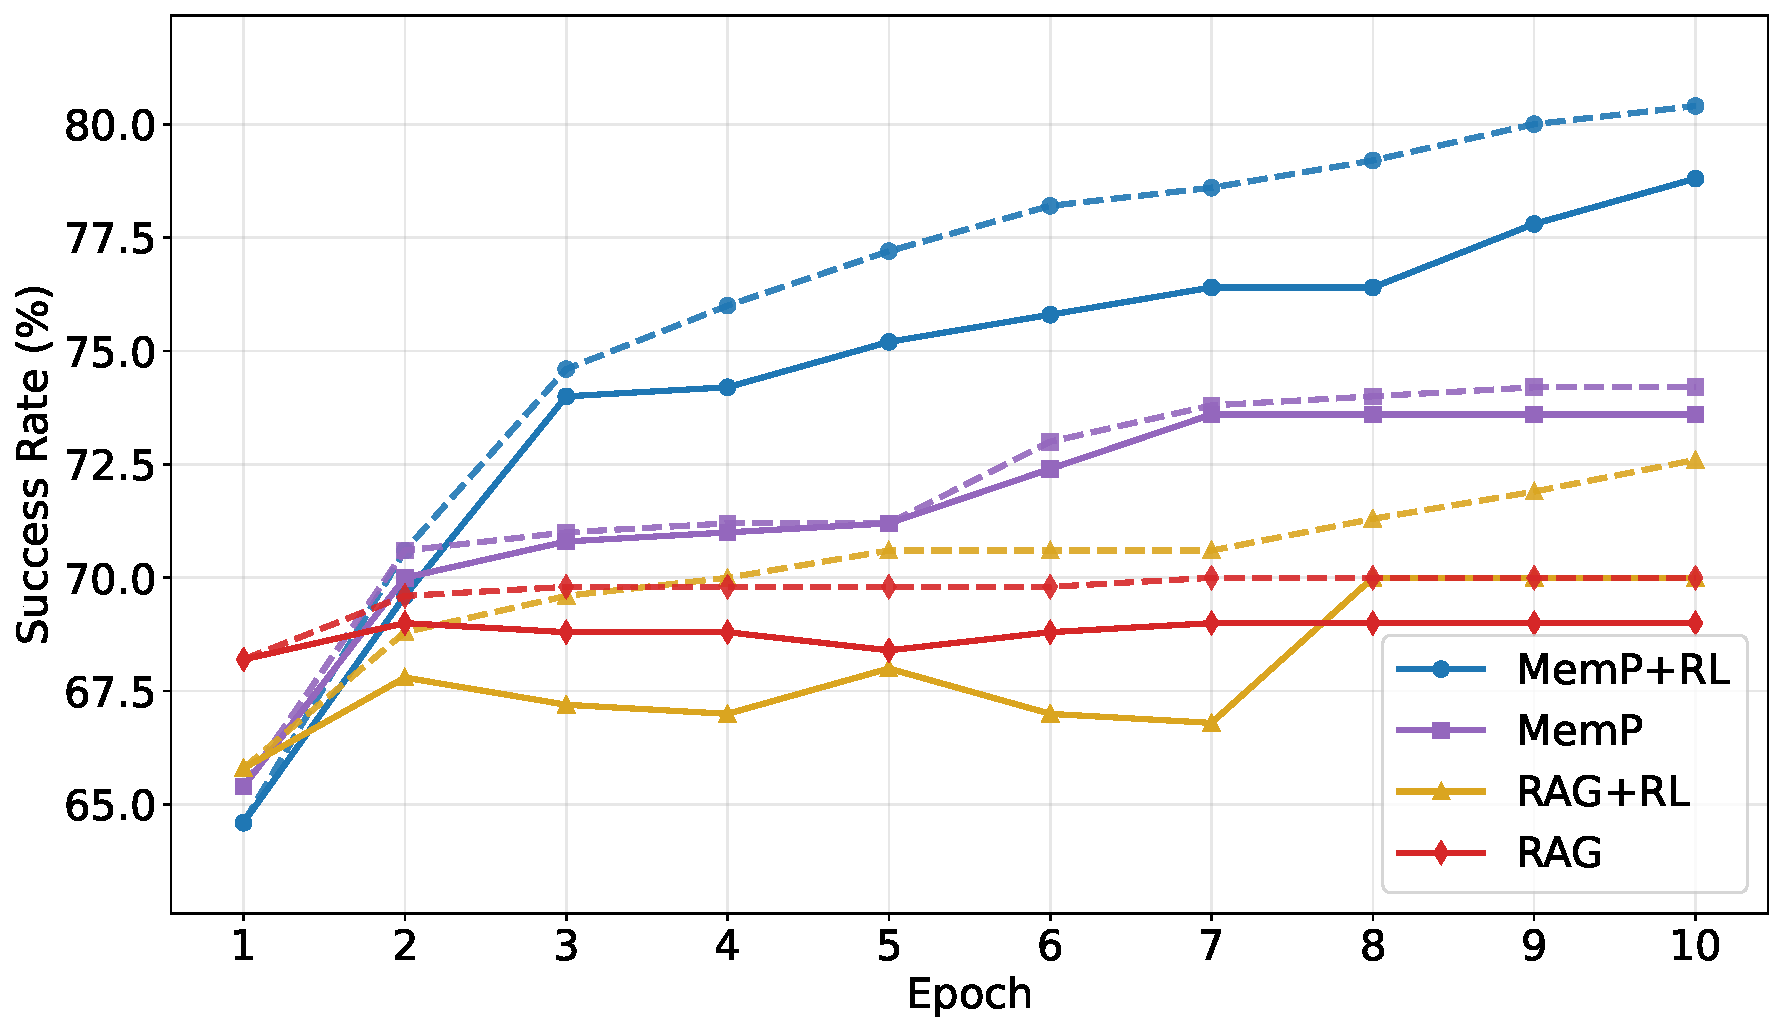
\includegraphics[width=0.8\linewidth]{success_and_cumulative_rate_curves.pdf}
    
    \caption{\textbf{OS Interaction Performance.} 
    Performance comparison of \textsc{MemRL} vs. baselines (MemP, RAG). \textbf{Solid lines} represent the Epoch Success Rate, while \textbf{dashed lines} indicate the Cumulative Success Rate (CSR). \textsc{MemRL} demonstrates superior stability and a widening performance gap in CSR.}
    \label{fig:os_performance_combined}
    \vskip -8pt
\end{figure}


To isolate the efficacy of runtime RL, we compare \textsc{MemRL} and its RAG-based variant against their non-RL counterparts (MemP and standard RAG) in the OS interaction environment. As shown in Figure~\ref{fig:os_performance_combined}, while initial performance is comparable, a clear divergence emerges as training progresses: \textsc{MemRL} achieves a smoother learning curve and superior stability.
Crucially, this advantage is most pronounced in the Cumulative Success Rate (dashed lines), where the monotonic widening gap indicates that the RL-driven value function effectively filters noisy memories and consolidates successful experiences.


% \subsubsection{Impact of Q-Value Weighting}

% To understand the interplay between semantic retrieval and reinforcement learning, we analyze the impact of the Q-weighting factor $\lambda$ in the scoring function, i.e., the Equation~\ref{eq:score}:

% We compare the balanced setting ($\lambda=0.5$) against two extremes: pure semantic retrieval ($\lambda=0$) and pure greedy RL ($\lambda=1$).

% \begin{figure}[t]
%     \centering

%     % --- 上图 ---
%     \begin{subfigure}{\linewidth}
%         \centering
%         % 固定高度以保证两张图严格对齐；keepaspectratio 避免变形
%         \includegraphics[width=\linewidth, height=5.0cm, keepaspectratio]{q_weight_ablation_success}
%         \caption{Success Rate}
%         \label{fig:q_weight_success}
%     \end{subfigure}

%     \vspace{0.6em} % 上下间距可调：0.3em~1.0em

%     % --- 下图 ---
%     \begin{subfigure}{\linewidth}
%         \centering
%         \includegraphics[width=\linewidth, height=5.0cm, keepaspectratio]{q_weight_ablation_cumulative}
%         \caption{Cumulative Success Rate}
%         \label{fig:q_weight_cumulative}
%     \end{subfigure}

%     \caption{\textbf{Ablation study on Q-value weighting factor $\lambda$.}
%     The balanced setting ($\lambda=0.5$) achieves superior stability and peak performance compared to extreme configurations.}
%     \label{fig:q_weight_ablation}

%     \vspace{-0.15in}
% \end{figure}

% As illustrated in Figure~\ref{fig:q_weight_ablation}, the \textbf{balanced configuration} consistently yields superior performance.
% This indicates that the combination of semantic grounding and utility-driven ranking effectively guides the agent towards high-quality solutions while maintaining context relevance.
% Besides, the \textbf{pure semantic retrieval baseline} provides a stable starting point but lacks the mechanism to filter out suboptimal memories that are semantically similar but functionally incorrect. 
% Consequently, its performance plateaus early, which highlights the necessity of the RL signal for continued improvement.
% On the other hand, the \textbf{pure RL setting} reveals the risks of disregarding semantic context, exhibiting significant instability and poor initial performance.
% We attribute this instability to \textit{context detachment}: without the constraint of semantic similarity, the agent may retrieve high-$Q$ memories (successful in other contexts) that are irrelevant to the current task. 
% This confirms that semantic similarity must act as an anchor for retrieval, while RL provides the necessary gradient for optimizing memory selection.
\subsubsection{Impact of Q-Value Weighting}
\label{sec:ablation_lambda}

\begin{figure}[t]
    \centering
    % 使用合并后的单张大图
    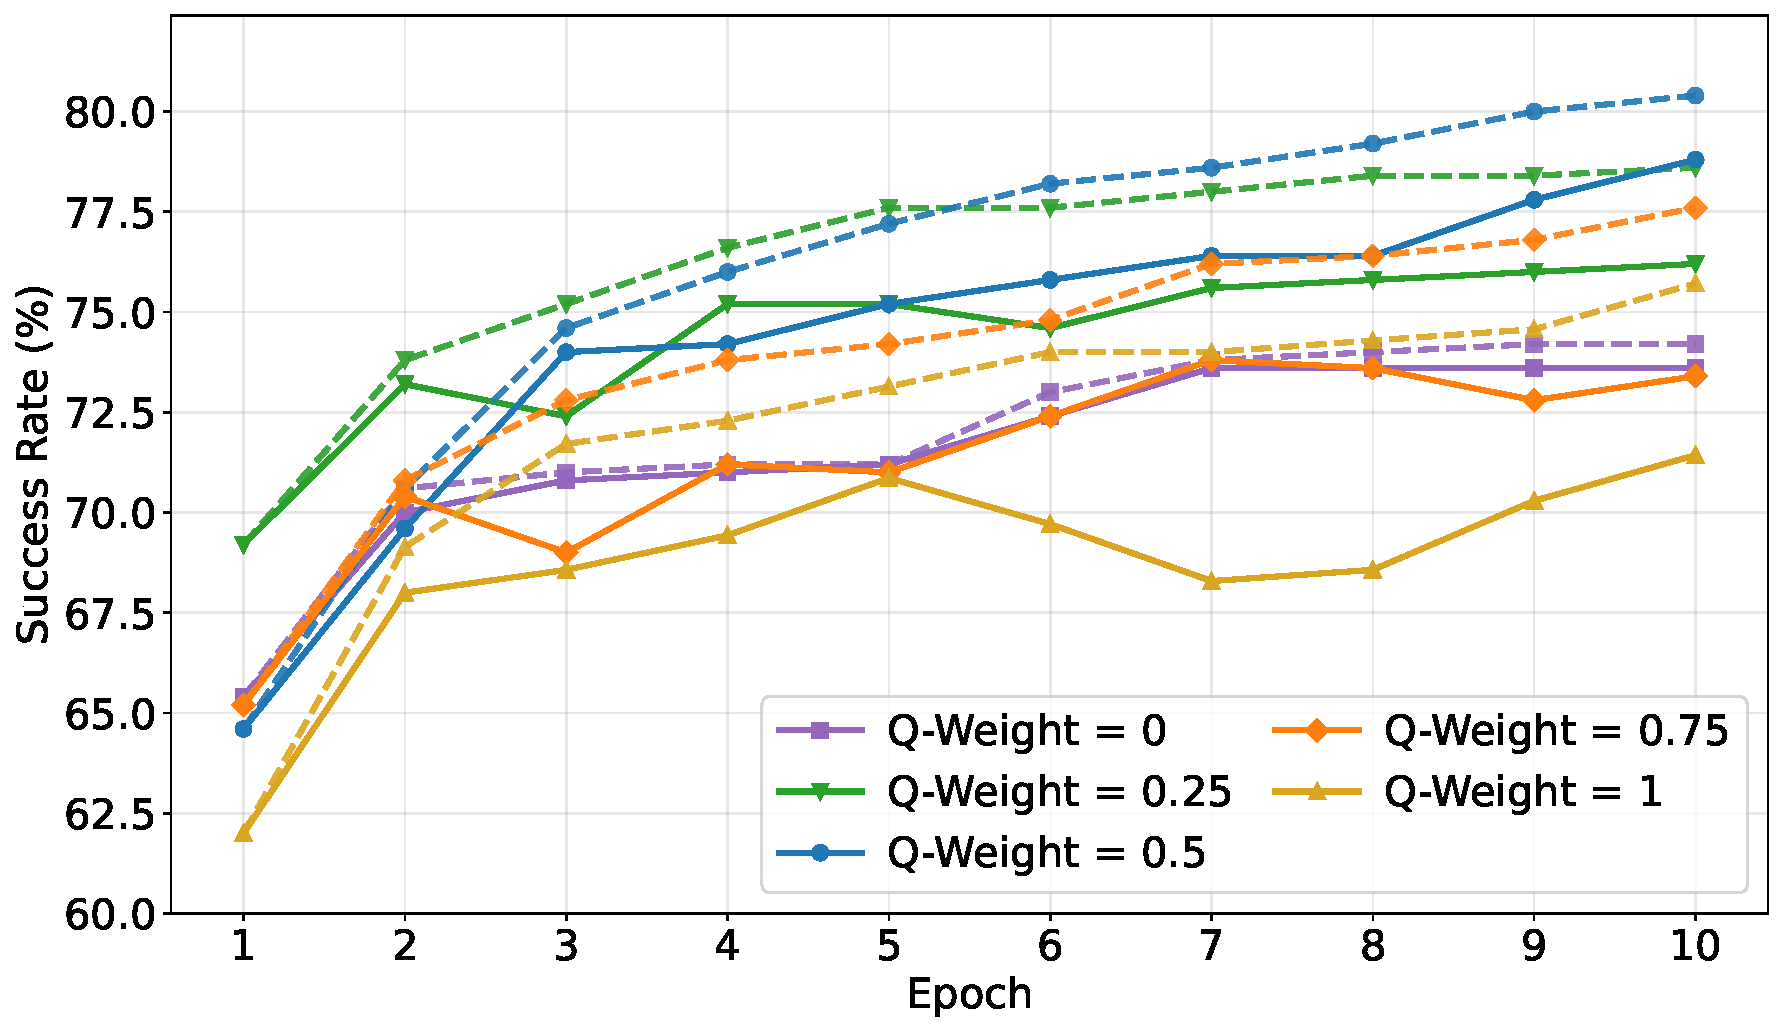
\includegraphics[width=0.8\linewidth]{success_and_cumulative_by_epoch_lamda.pdf}
    
    \caption{\textbf{Ablation on Q-value weighting factor $\lambda$.} 
    Performance comparison across $\lambda \in \{0, 0.25, 0.5, 0.75, 1\}$. \textbf{Solid lines} denote Epoch Success Rate, while \textbf{dashed lines} indicate Cumulative Success Rate (CSR). The balanced setting ($\lambda=0.5$) achieves the optimal trade-off between relevance and helpfulness.}
    \label{fig:q_weight_ablation}
    
    \vskip -0.15in
\end{figure}

To determine the optimal equilibrium between semantic grounding and value-based exploitation, we evaluate the Q-weighting factor $\lambda \in \{0, 0.25, 0.5, 0.75, 1\}$. As shown in Figure~\ref{fig:q_weight_ablation}, performance exhibits a clear concave trend peaking at $\lambda=0.5$. Deviating toward extremes degrades results: pure semantic retrieval ($\lambda=0$) plateaus due to an inability to filter functional distractors, while excessive RL weight ($\lambda \to 1$) induces volatility and context detachment. This confirms that $\lambda=0.5$ represents an effective balance, where semantic similarity guarantees content relevance and Q-value ensures its helpfulness.



\begin{table}[h]
\centering
\caption{\textbf{Ablation on Retrieval Scope.} We compare \textsc{MemRL} against an ablated version restricted to \textit{Single-Task Reflection}.}
\label{tab:ablation_scope}
\resizebox{\linewidth}{!}{%
\begin{tabular}{l c c c c c | c}
\toprule
\textbf{Setting} & \textbf{BCB} & \textbf{OS} & \textbf{DB} & \textbf{ALFWorld} & \textbf{HLE} & \textbf{Avg.} \\
\midrule
Single-Task Reflection & 0.614 & 0.714 & 0.938 & 0.930 & \textbf{0.610} & 0.761 \\
\textbf{\textsc{MemRL} (Cross-Task)} & \textbf{0.627} & \textbf{0.804} & \textbf{0.972} & \textbf{0.981} & 0.606 & \textbf{0.798} \\
\bottomrule
\end{tabular}%
}
% \vskip -0.2in
\end{table}

\subsubsection{Ablation Analysis: Cross-Task vs. Single-Task Optimization}
\label{sec:ablation_scope}

To investigate the source of our performance gains, we conduct an ablation study in Table~\ref{tab:ablation_scope} by restricting the memory retrieval scope. We compare the full \textsc{MemRL} (\textit{Cross-Task Retrieval}) against an ablated setting that only utilizes feedback from the single task instance, conceptually equivalent to Reflexion \citep{shinn2023reflexion}. \textsc{MemRL} demonstrates superior performance in structured environments, particularly on \textbf{OS-Agent} ($+9.0\%$) and \textbf{ALFWorld} ($+5.1\%$). These benchmarks exhibit high intra-dataset similarity, allowing \textsc{MemRL} to effectively perform \textit{horizontal transfer}—retrieving and adapting successful policies from semantically similar historical tasks. While on the HLE benchmark, the single-task baseline ($0.610$) is tied with \textsc{MemRL} ($0.606$). We attribute this to the HLE dataset's low internal semantic similarity ($0.186$), as detailed in Appendix~\ref{app:sim-analysis}. This prevents effective cross-task generalization, forcing the agent to rely solely on single feedback.

\subsubsection{Sensitivity to Retrieval Size ($k_1$ and $k_2$).}

\begin{figure}[t]
    \centering
    \begin{subfigure}{\linewidth}
        \centering
        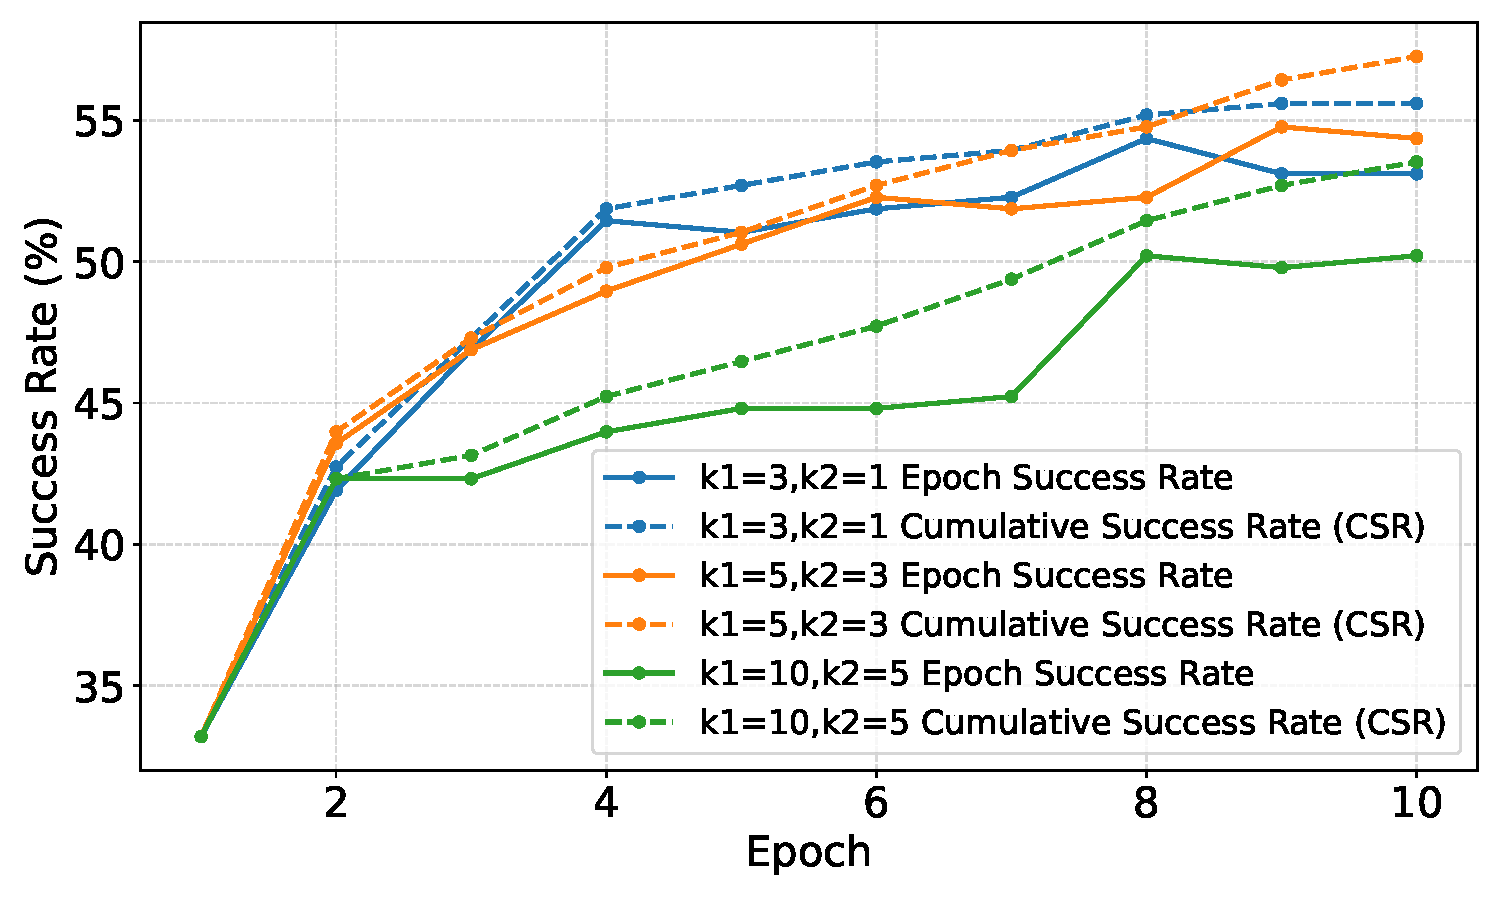
\includegraphics[width=0.8\linewidth, height=5.0cm, keepaspectratio]{hle_k1k2.pdf}
    \end{subfigure}
    \caption{\textbf{Ablation on Retrieval Size ($k_1, k_2$).}
    Performance comparison on the HLE (CS/AI) subset across sparse ($3/1$), moderate ($5/3$), and dense ($10/5$) retrieval settings. The moderate setting achieves the optimal trade-off.}
    \label{fig:ablation_k}
    \vskip -0.15in
\end{figure}

To investigate the impact of retrieval bandwidth, we compare three memory density configurations on the HLE (CS/AI) subset benchmark: sparse ($k_1=3, k_2=1$), moderate ($k_1=5, k_2=3$), and dense ($k_1=10, k_2=5$). As shown in Figure \ref{fig:ablation_k}, performance follows an inverted-U trajectory, illustrating the trade-off between information sufficiency and context noise. The sparse setting limits performance due to insufficient guidance, whereas the dense setting degrades success rate by introducing distractions into the reasoning context. Consequently, the moderate configuration ($k_1=5, k_2=3$) achieves the best result, effectively maximizing the signal-to-noise ratio of the retrieved context.
% \begin{figure}[t]
%     \centering
%     % 使用 minipage 限制整个区域的宽度为 0.5 (和上面的子图一致)
%     \begin{minipage}{0.5\linewidth}
%         \centering
%         % 这里设为 1.0 表示填满这个 0.5 的容器
%         \includegraphics[width=\linewidth]{hle_k_compare.pdf}
        
%         \caption{\textbf{Ablation on Retrieval Size ($k_1, k_2$).} 
%         Performance (acc: Epoch-Acc; cum: Cumulative Acc) comparison on HLE (CS/AI) across different retrieval counts.}
%         \label{fig:ablation_k}
%     \end{minipage}
    
%     \vspace{-0.15in}
% \end{figure}
% \begin{figure}[t]
%     \centering

%     \begin{subfigure}{\linewidth}
%         \centering
%         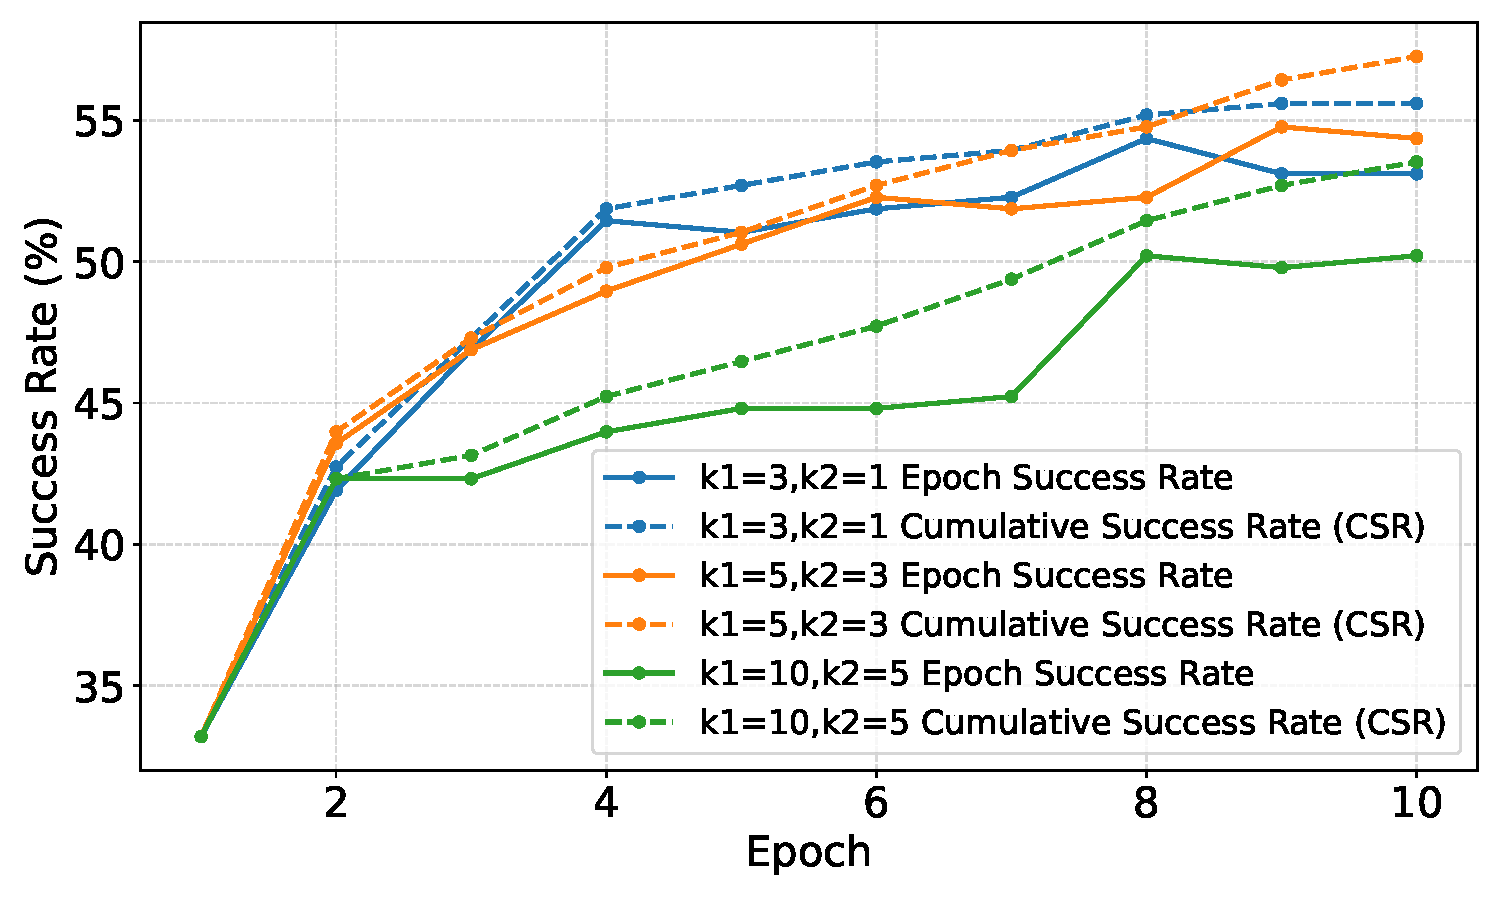
\includegraphics[width=\linewidth, height=5.0cm, keepaspectratio]{hle_k1k2.pdf}
%     \end{subfigure}

%     \caption{\textbf{Ablation on Retrieval Size ($k_1, k_2$).}
%     Performance comparison on HLE (CS/AI) across different retrieval counts.}
%     \label{fig:ablation_k}

%     \vspace{-0.15in}
% \end{figure}

% To investigate the impact of memory capacity on reasoning performance, we conducted an ablation study on a subset of the HLE benchmark (Computer Science/AI category). We compared two retrieval configurations: a larger recall setting ($k_1=10, k_2=5$) and a compact recall setting ($k_1=5, k_2=3$).  
% As shown in Figure \ref{fig:ablation_k}, the compact setting ($k_1=5, k_2=3$) achieves superior stability compared to the larger setting, suggesting that for complex reasoning tasks like HLE, simply increasing context volume can introduce irrelevant noise that interferes with the model's judgment. Therefore, a smaller, higher-quality set of retrieved memories is sufficient for maintaining reasoning precision.  
% 检索的质量高-不需要过多memory-浪费-噪声





\subsection{Discussion}

In this section, we delve deeper into the mechanisms driving \textsc{MemRL}'s performance, connecting empirical results to the challenge of balancing knowledge retention and adaptation.

% \subsubsection{\textsc{MemRL} as a Trajectory Verifier.}

% % --- 文字环绕开始 ---
% % 宽度设为 0.6\textwidth 以容纳 "BigCodeBench" 这种长词
% % \begin{wraptable}{r}{0.6\textwidth}
% %     \vspace{-0.25in} % 对齐第一行文字
% %     \centering
% %     \footnotesize  % 改用 footnotesize 保证长词能放下
% %     \setlength{\tabcolsep}{1.5pt} % 稍微收紧列间距
    
% %     \caption{\textbf{Impact of Task Structure.} Comparison of Cumulative Success Rate (CSR) gains. Multi-step tasks benefit significantly more from MemRL.}
% %     \label{tab:horizon_analysis}
    
% %     \begin{tabular}{@{}l l c c c@{}}
% %         \toprule
% %         \textbf{Benchmark} & \textbf{Interaction} & \textbf{MemP} & \textbf{MemRL} & \textbf{Gain} \\
% %         & & \textbf{(\%)} & \textbf{(\%)} & \textbf{(pp)} \\
% %         \midrule
% %         ALFWorld     & Multi-step  & 45.6 & \textbf{69.7} & \textbf{+24.1} \\
% %         OS Task      & Multi-step  & 74.3 & \textbf{81.7} & \textbf{+7.4}  \\
% %         HLE          & Single-step & 58.2 & 61.3 & +3.1 \\
% %         BigCodeBench & Single-step & 60.2 & 62.7 & +2.5 \\
% %         \bottomrule
% %     \end{tabular}
% %     \vspace{-0.1in}
% % \end{wraptable}
% \begin{table}[b]  % t / h / b / H 按需要调
%     \centering
%     \footnotesize
%     \setlength{\tabcolsep}{1.5pt}

%     \caption{\textbf{Impact of Task Structure.} Comparison of Cumulative Success Rate (CSR) gains. Multi-step tasks benefit significantly more from \textsc{MemRL}.}
%     \label{tab:horizon_analysis}

%     \begin{tabular}{@{}l l c c c@{}}
%         \toprule
%         \textbf{Benchmark} & \textbf{Interaction} & \textbf{MemP (\%)} & \textbf{\textsc{MemRL} (\%)} & \textbf{Gain (pp)} \\
%         % & & \textbf{(\%)} & \textbf{(\%)} & \textbf{(pp)} \\
%         \midrule
%         ALFWorld     & Multi-step  & 45.6 & \textbf{69.7} & \textbf{+24.1} \\
%         OS Task      & Multi-step  & 74.3 & \textbf{81.7} & \textbf{+7.4}  \\
%         HLE          & Single-step & 58.2 & 61.3 & +3.1 \\
%         BigCodeBench & Single-step & 60.2 & 62.7 & +2.5 \\
%         \bottomrule
%     \end{tabular}
% \end{table}
% % --- 表格结束 ---

% Table~\ref{tab:horizon_analysis} reveals a correlation between task structural complexity and performance gain. The gains are most profound in multi-step sequential tasks (e.g., ALFWorld +24.1 Percentage Points(pp)) compared to single-turn tasks (e.g., BigCodeBench +2.5 pp).
% In sequential tasks, a retrieved memory must be valid for the \textit{entire} trajectory. Standard semantic retrieval often fetches memories that match the initial instruction but fail in later steps. By propagating the final reward backward to the memory utility $Q$, \textsc{MemRL} effectively learns to verify the \textit{whole trajectory}, filtering out brittle policies that look correct only on the surface.

% This analysis indicates that \textsc{MemRL} transcends the role of a simple retrieval enhancer to function as a \textit{Trajectory Verifier}. Its value is maximized in tasks with complex temporal dependencies, where it learns to select memories that ensure the structural integrity of the entire interaction process.



\subsubsection{Predictive Power of the Q Critic}
% \begin{figure}[b!]
%     \centering
    
%     % --- 第一个子图 (左) ---
%     \begin{subfigure}{0.48\linewidth}
%         \centering
%         % 这里的 \linewidth 指的是子图容器的宽度(即页面的48%)
%         % 这样设置能让图最大化利用半栏空间
%         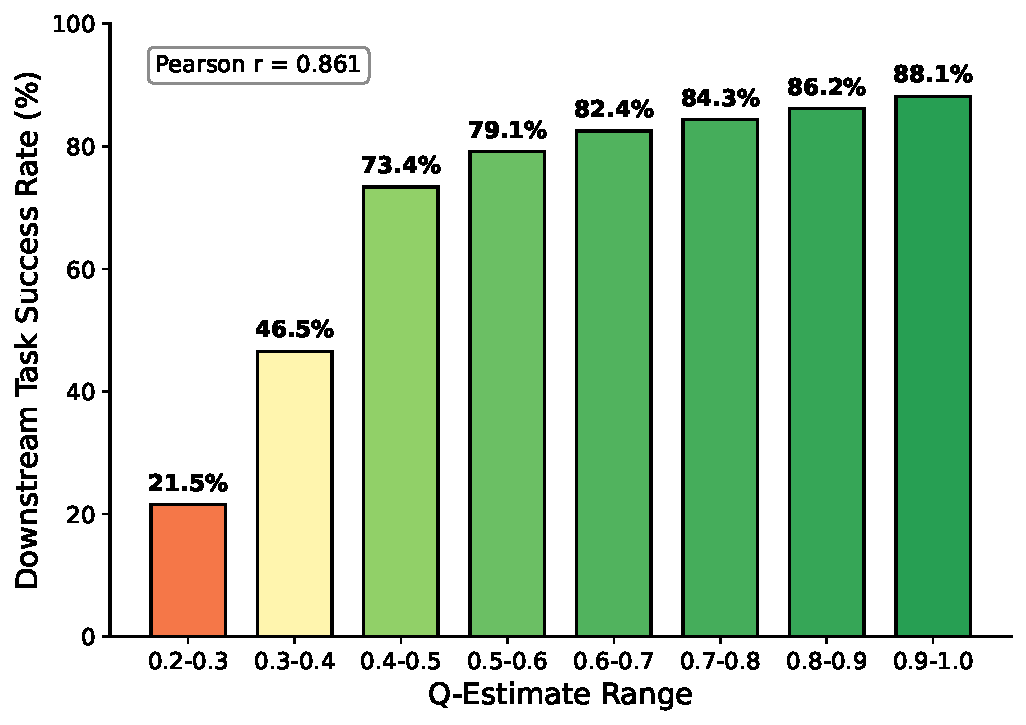
\includegraphics[width=\linewidth]{q_predictive_power}
%         \caption{Success Rate vs. Q-Range}
%         \label{fig:q_correlation}
%     \end{subfigure}
%     \hfill
%     % --- 第二个子图 (右) ---
%     \begin{subfigure}{0.48\linewidth}
%         \centering
%         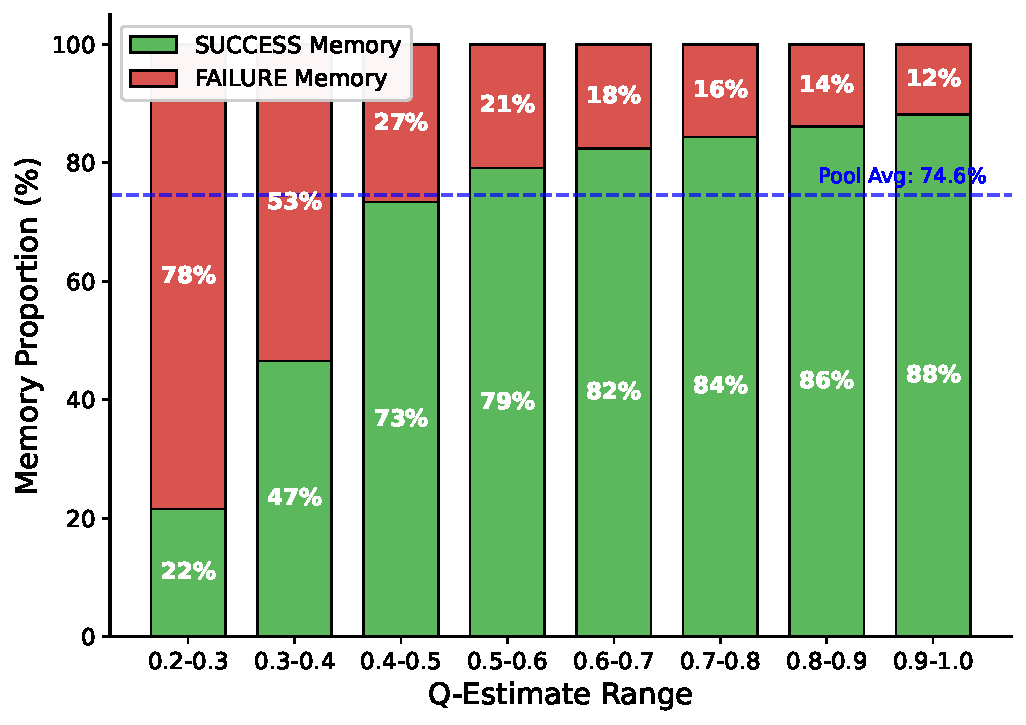
\includegraphics[width=\linewidth]{memory_composition}
%         \caption{Memory Composition}
%         \label{fig:q_composition}
%     \end{subfigure}
    
%     \caption{\textbf{Q-Value Analysis.} (a) Pearson $r=0.861$ confirms Critic's predictive power. (b) Failure memories ($\sim12\%$) in high Q-bins indicate latent strategic utility.}
%     \label{fig:q_value_analysis}
    
%     % --- 底部间距 ---
%     \vspace{-0.15in} 
% \end{figure}

\begin{figure}[t]
    \centering
    % --- 子图 1 (左) ---
    \begin{subfigure}[b]{0.8\linewidth}
        \centering
        % 移除固定高度，让宽度自适应，或者根据需要保留 height
        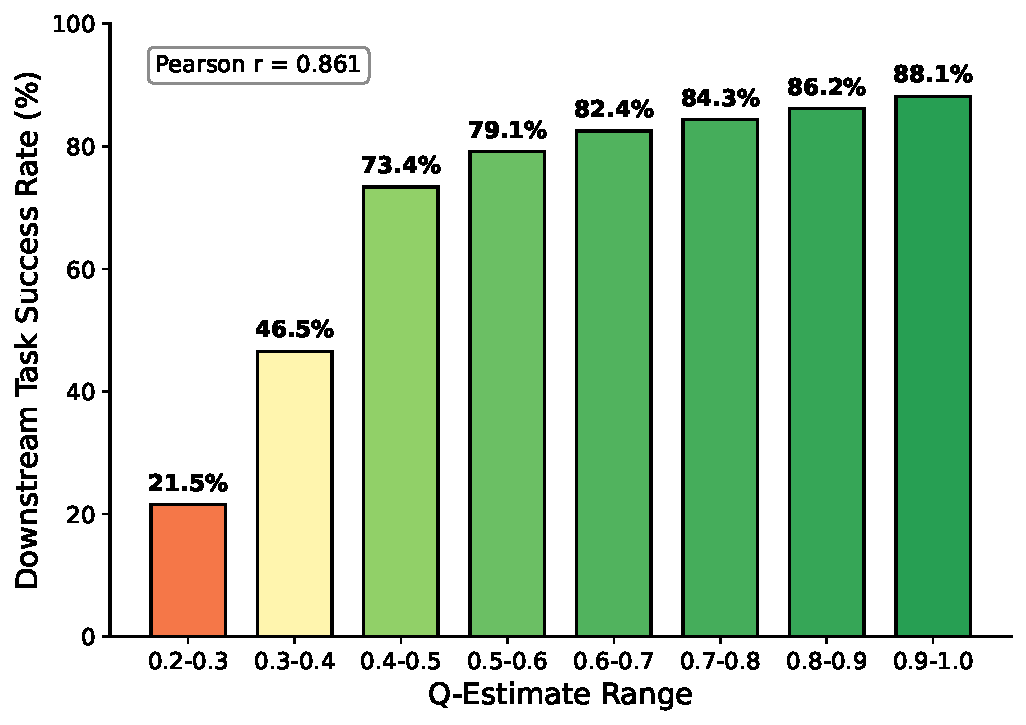
\includegraphics[width=\linewidth]{q_predictive_power}
        \vskip -4pt
        \caption{Success Rate vs. Q-Range}
        \label{fig:q_correlation}
    \end{subfigure}
    \hfill % 关键：撑开两个子图之间的距离
    % --- 子图 2 (右) ---
    \begin{subfigure}[b]{0.8\linewidth}
        \centering
        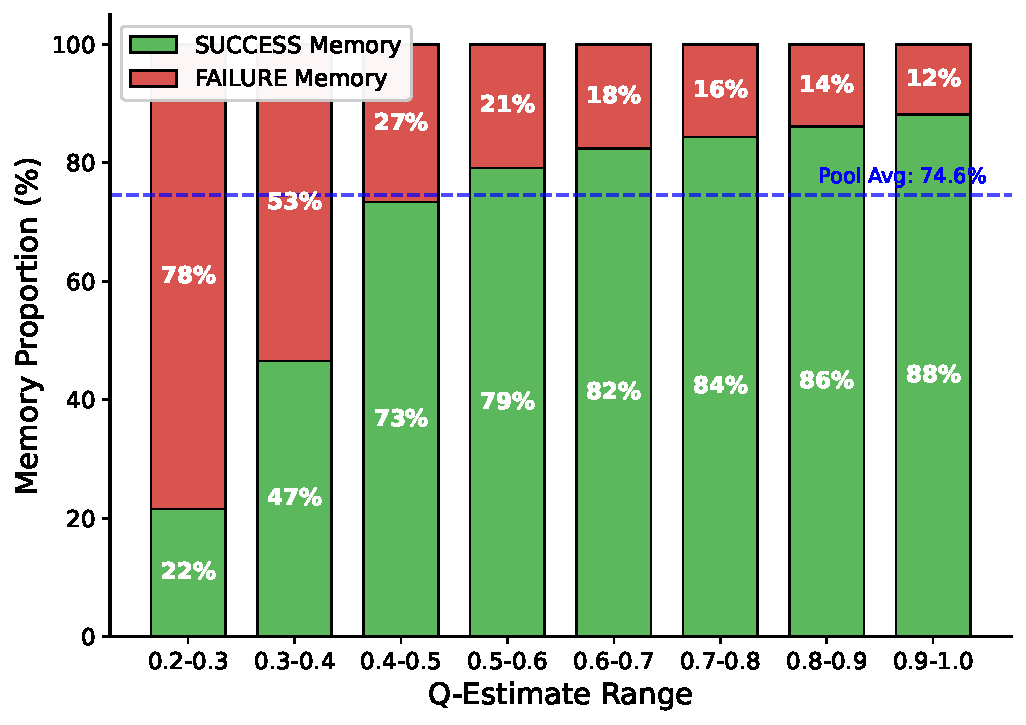
\includegraphics[width=\linewidth]{memory_composition}
        \vskip -4pt
        \caption{Memory Composition}
        \label{fig:q_composition}
    \end{subfigure}

    % \vspace{-0.5em} % 稍微调整 caption 与图片之间的距离

    \caption{\textbf{Q-Value Analysis.} (a) Pearson $r=0.861$ confirms Critic's predictive power. (b) Failure memories ($\sim12\%$) in high Q-bins indicate latent strategic utility.}
    \label{fig:q_value_analysis}
    \vskip-10pt
    
\end{figure}

% \begin{figure}[b!]
%     \centering

%     % --- 子图 1 (上) ---
%     \begin{subfigure}{\linewidth}
%         \centering
%         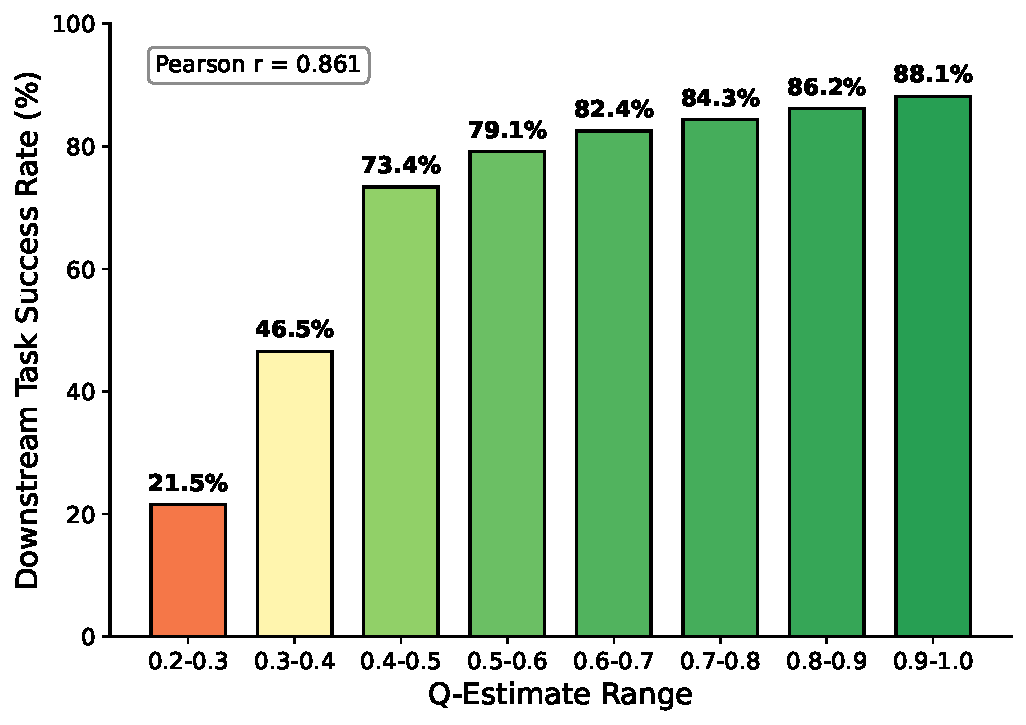
\includegraphics[width=\linewidth, height=5.0cm, keepaspectratio]{q_predictive_power}
%         \caption{Success Rate vs. Q-Range}
%         \label{fig:q_correlation}
%     \end{subfigure}

%     \vspace{0.6em}

%     % --- 子图 2 (下) ---
%     \begin{subfigure}{\linewidth}
%         \centering
%         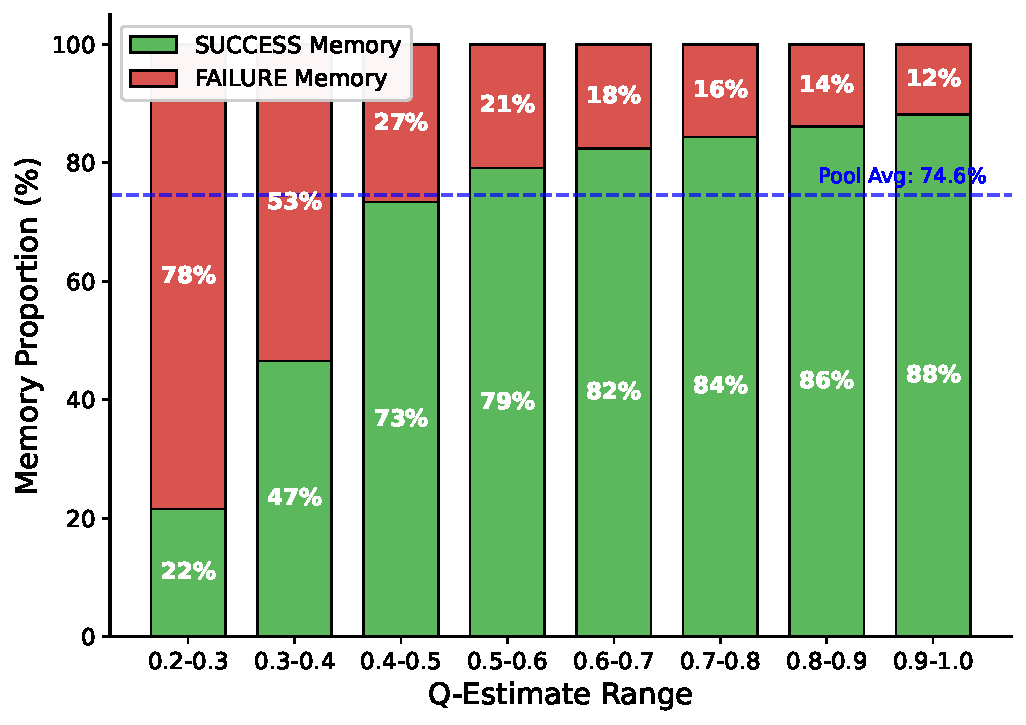
\includegraphics[width=\linewidth, height=5.0cm, keepaspectratio]{memory_composition}
%         \caption{Memory Composition}
%         \label{fig:q_composition}
%     \end{subfigure}

%     \caption{\textbf{Q-Value Analysis.} (a) Pearson $r=0.861$ confirms Critic's predictive power. (b) Failure memories ($\sim12\%$) in high Q-bins indicate latent strategic utility.}
%     \label{fig:q_value_analysis}

%     \vspace{-0.15in}
% \end{figure}

As shown in Figure~\ref{fig:q_correlation}, the learned Q-values exhibit a strong positive correlation (Pearson $r=0.861$) with empirical task success rates, rising from $21.5\%$ in the lowest-confidence bin to $88.1\%$ in the highest, which confirms the Critic's ability to effectively rank memories by success likelihood. 
Beyond simple ranking, memory composition analysis (Figure~\ref{fig:q_composition}) reveals that the agent retains a small fraction of ``failure'' memories ($\sim12\%$) even in high-Q bins ($0.9-1.0$), suggesting that Q-values capture \emph{utility beyond binary outcomes} by recognizing strategically useful near-misses. 
We further substantiate this with concrete case studies in Appendix~\ref{app:case}.
This indicates that the Critic prioritizes reusable guidance---including transferable procedural lessons from high-utility failures---rather than merely separating success from failure, thereby offering greater robustness than simple success-replay mechanisms.
% Does the learned Q-value truly reflect solution quality? Figure~\ref{fig:q_correlation} shows a strong positive correlation (Pearson $r=0.861$) between the Critic's estimated Q-values and empirical task success rates. The success rate increases from 21.5\% in the lowest-confidence bin to 88.1\% in the highest, indicating that a major driver of performance is the Critic's ability to rank memories by their likelihood of leading to successful task completion.

% Further analysis of memory composition (Figure~\ref{fig:q_composition}) suggests a secondary source of gain: robustness. Even in high-Q bins ($0.9$--$1.0$), the agent retains a small fraction of memories labeled as ``failure'' ($\sim$12\%). Rather than contradicting the Critic, this pattern is consistent with the interpretation that Q-values can capture \emph{utility beyond binary outcomes}: some unsuccessful trajectories remain strategically useful because they encode near-correct reasoning and transferable procedural lessons.

% Taken together, these results suggest that the Critic is not merely separating ``success'' from ``failure,'' but assigning higher value to memories that provide reusable guidance---including a subset of high-utility failures that are near-miss in nature. By retaining and reusing such corrective heuristics, the agent can be more robust than simple success-replay mechanisms.

% \paragraph{Case study: a high-Q ``failure'' memory as a transferable near-miss.}
% We find high-Q failure memories that summarize a minor, localized mistake and a corrective heuristic that generalizes across tasks. Here we use \emph{near-miss} to denote trajectories that are largely correct but fail due to minor, localized errors (e.g., verification slips or tool-usage details). For example, one failure memory with $Q=0.9878$ corresponds to a trajectory that followed a correct approach but incorrectly treated an \emph{empty command output} as evidence of failure. The stored reflection explicitly identifies the root cause (misinterpreting empty output), warns against the pattern (equating ``no output'' with failure), and recommends the correct approach (validate success via exit status, error logs, or other objective signals). When retrieved in later episodes, this single ``failure'' memory supports perfect downstream outcomes in our logs (15/15 successes), demonstrating that the memory is valuable precisely because it captures a fixable near-miss rather than an uninformative failure.







% 正向迁移与遗忘探讨+如何找到高质量的记忆，到底是哪些记忆在起作用？（正负pattern）(HLE) zst

\subsubsection{Stability of \textsc{MemRL}}
\label{sec:stable in mem rl exp}

We analyze \textsc{MemRL} through the lens of the \textit{stability-plasticity dilemma}. The superior CSR (Table~\ref{tab:runtime_main_results}) confirms that \textsc{MemRL} effectively expands the solution space, enabling the agent to break through local optima. Furthermore, long-term dynamics (Figure~\ref{fig:acc_gap}) reveal a critical stability advantage: while heuristic methods like MemP suffer from catastrophic forgetting—evidenced by a widening gap between CSR and current Success Rate—\textsc{MemRL} maintains synchronized growth. This is theoretically guaranteed by our stability analysis in Section~\ref{sec:stability}, which constrains the policy to improve monotonically without drift.

\begin{figure}[t]
    \centering
    \begin{subfigure}{0.8\linewidth}
        \centering
        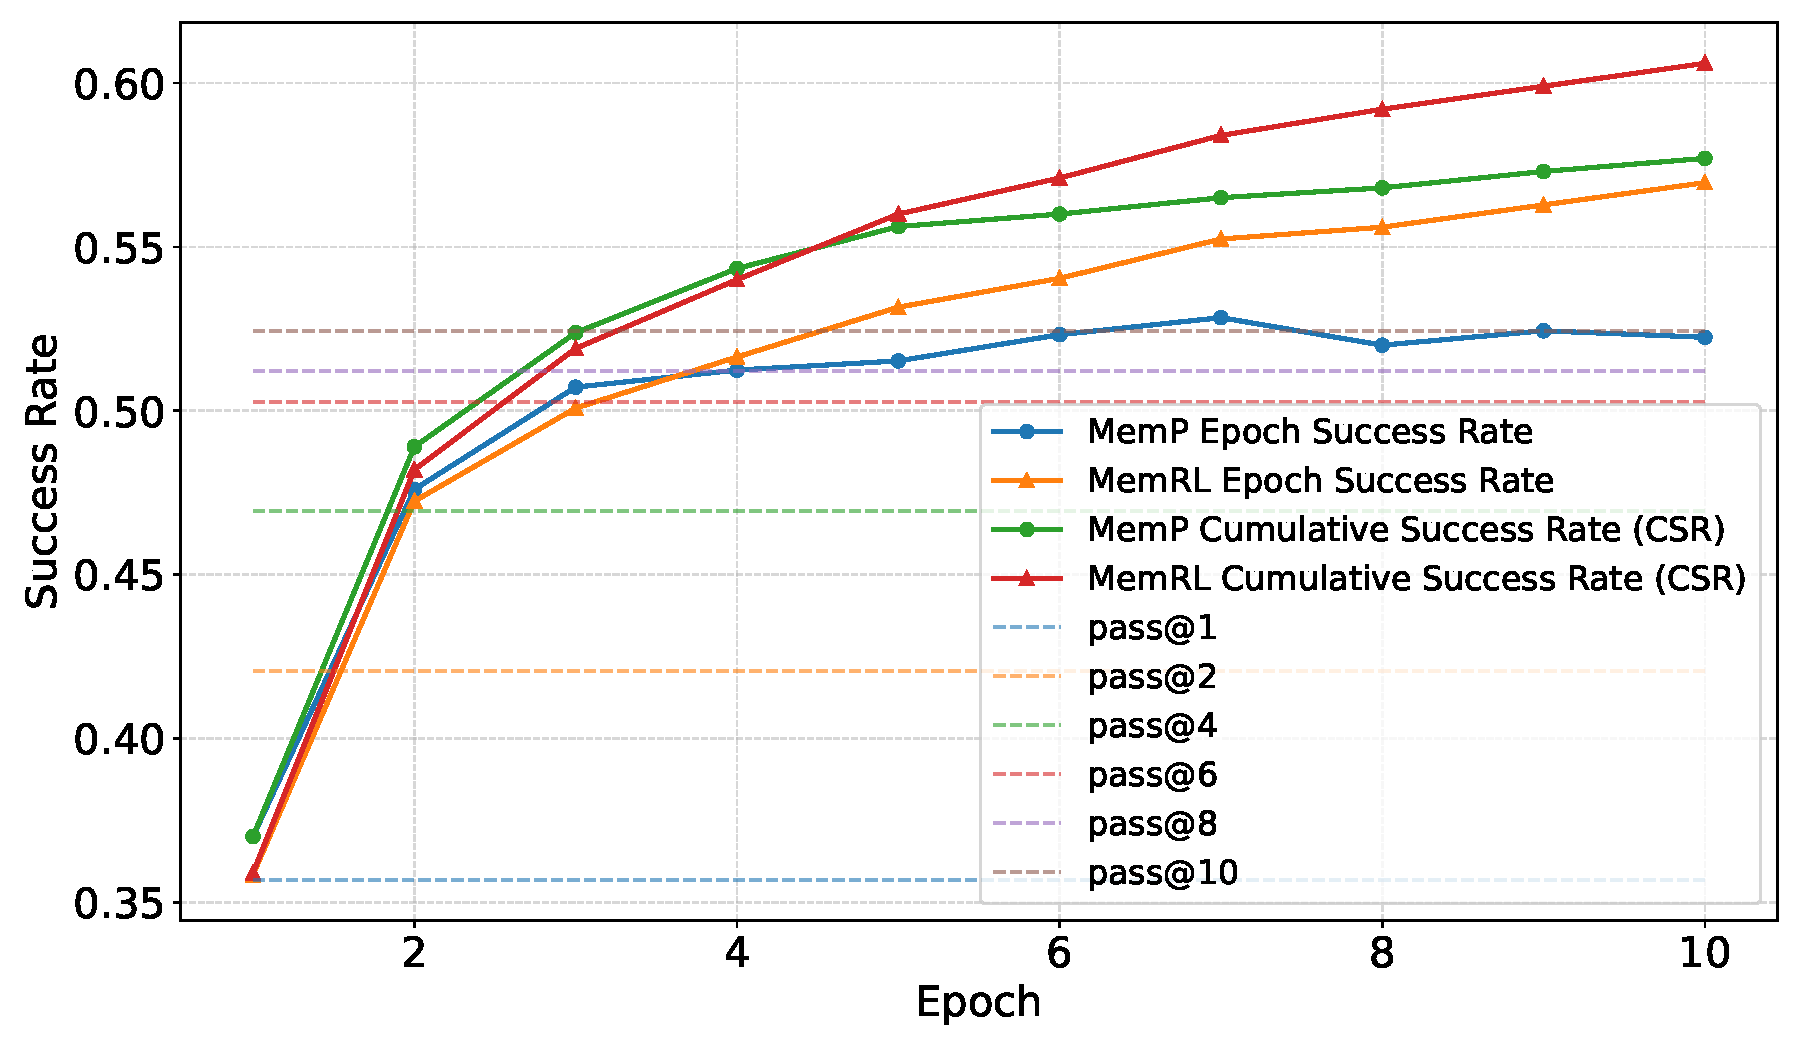
\includegraphics[width=\linewidth, height=5.5cm, keepaspectratio]{hle_memp_rl.pdf}
    \end{subfigure}
    \vskip -4pt
    \caption{Epoch Success Rate and Cumulative Success Rate (CSR) of \textsc{MemRL} and MemP in HLE.}
    \label{fig:acc_gap}
    \vskip -6pt
    % \vspace{-0.15in}
\end{figure}

% We quantitatively validate these insights using the \textbf{Forgetting Rate} (see Figure~\ref{fig:transfer-forget} in Appendix~\ref{app:forgetting_dynamics} for the full trajectory). \textsc{MemRL} achieves the lowest mean forgetting rate ($0.041$), outperforming the MemP ($0.051$). Additionally, ablation results demonstrate that removing z-score normalization and similarity gating causes the rate to spike to $0.073$. This confirms that strict filtering is essential to manage utility variance and ensure that self-evolution remains stable while maximizing positive transfer.
We quantitatively validate these insights using the \textbf{Forgetting Rate}, defined as $FR = N_{\text{lost}} / N_{\text{fail}}$, where $N_{\text{lost}}$ denotes tasks transitioning from previous success to current failure and $N_{\text{fail}}$ is the total number of failures in the current epoch (see Figure~\ref{fig:transfer-forget} in Appendix~\ref{app:forgetting_dynamics} for the full trajectory). \textsc{MemRL} achieves the lowest mean forgetting rate ($0.041$), outperforming \textsc{MemP} ($0.051$). Additionally, ablation results demonstrate that removing z-score normalization and similarity gating causes the rate to spike to $0.073$. This confirms that strict filtering is essential to manage utility variance and ensure that self-evolution remains stable.
\subsubsection{Extended Analysis.} 
We conduct further investigations to characterize the underlying mechanisms and generalization of \textsc{MemRL}. Specifically, Appendix~\ref{app:analysis} analyzes \textsc{MemRL}'s role as a structural trajectory verifier and the correlation between task similarity and performance gains. Additionally, evaluations of advanced capabilities---including cross-model memory transferability and modular multi-task merging---are detailed in Appendix~\ref{app:advanced_exp}, demonstrating \textsc{MemRL}'s versatility and its capacity for modular capability expansion. We also analyze the cost and efficiency of \textsc{MemRL} in Appendix~\ref{app:efficiency_analysis}.



% \subsubsection{Stability of \textsc{MemRL}}
% \label{sec:stable in mem rl exp}

% We analyze the underlying mechanisms of \textsc{MemRL} through the view of the \textit{stability-plasticity dilemma}, examining how our framework balances the acquisition of new capabilities with the retention of established knowledge.

% The superior CSR (Table~\ref{tab:runtime_main_results}) demonstrates that \textsc{MemRL} effectively expands the agent's solution space. Unlike heuristic baselines constrained by static similarity, which often retrieve redundant nearest neighbors leading to repeated failures, \textsc{MemRL} allows the agent to identify and reinforce non-obvious but effective strategies. This capability enables the agent to break through local optima where traditional retrieval methods stagnate.

% \begin{figure}[t]
%     \centering
%     \begin{subfigure}{0.95\linewidth}  % 这里调 0.85~0.95 都行
%         \centering
%         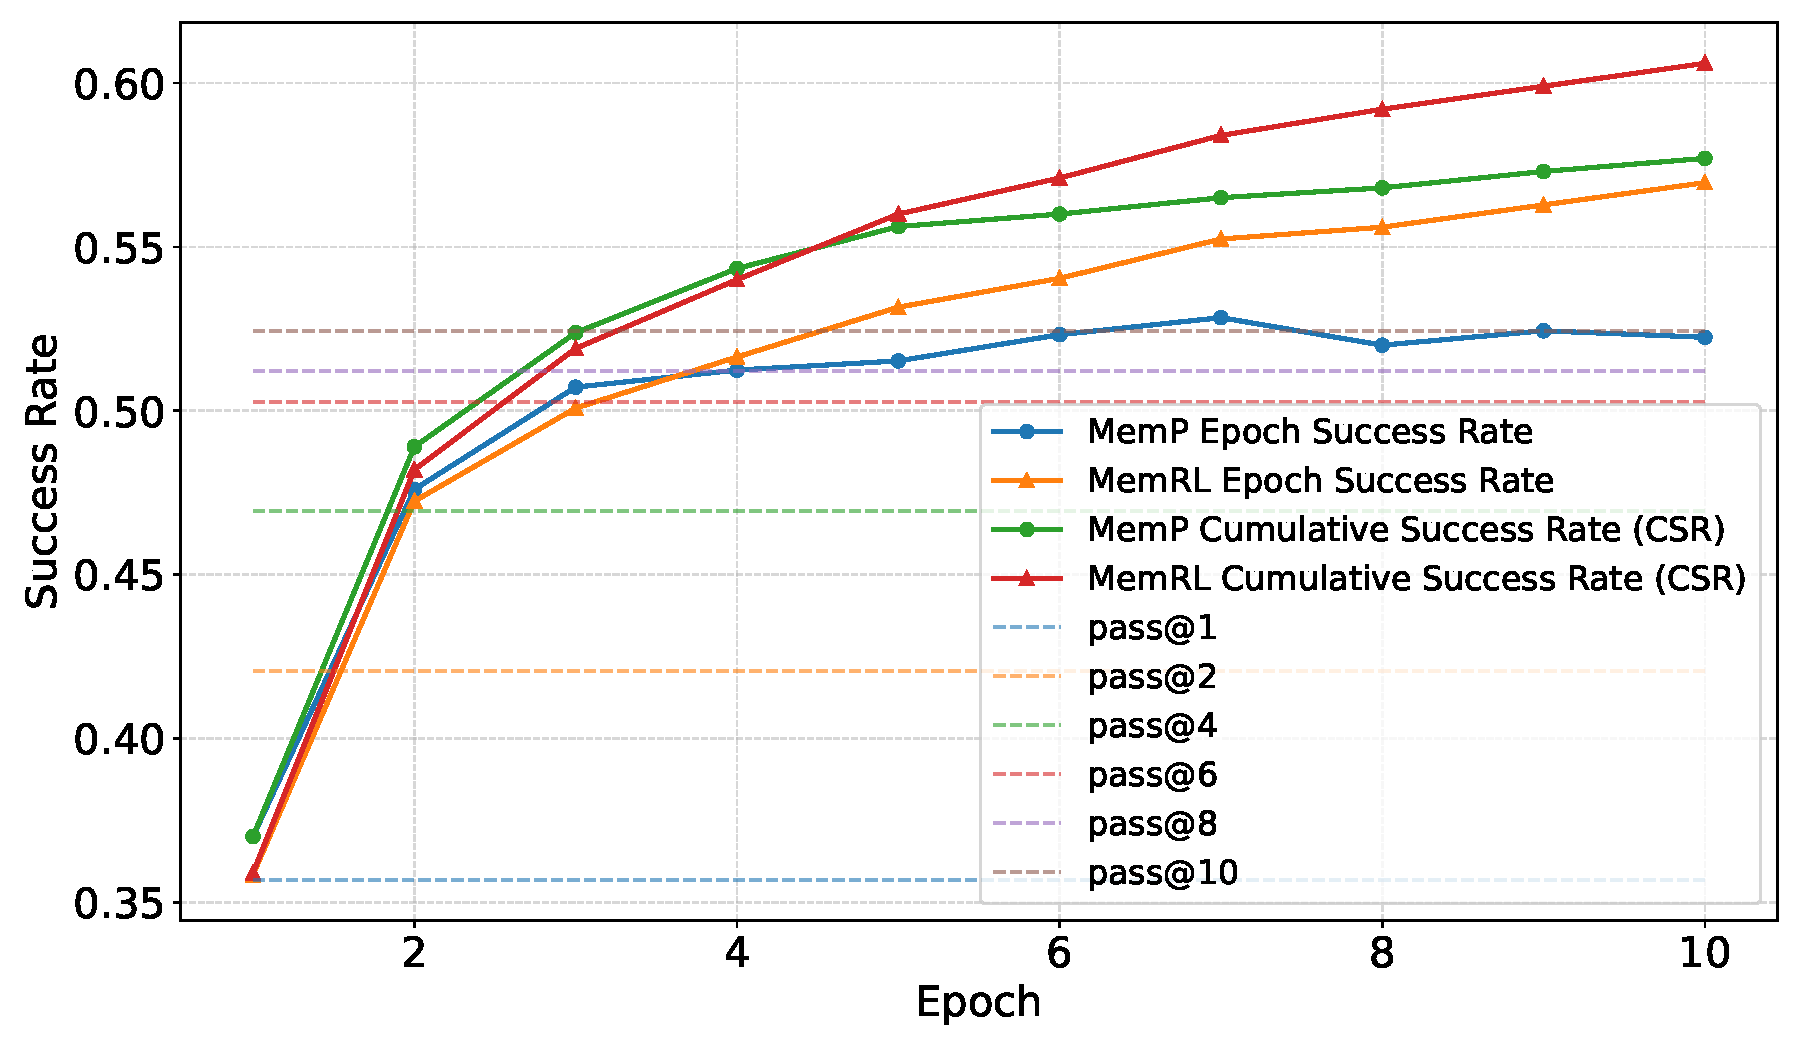
\includegraphics[width=\linewidth, height=5.5cm, keepaspectratio]{hle_memp_rl.pdf}
%     \end{subfigure}
%     \caption{Epoch Acc and Cumulative Acc of \textsc{MemRL} and MemP in HLE.}
%     \label{fig:acc_gap}

%     \vspace{-0.15in}
% \end{figure}



% Besides, long-term training dynamics (Figure~\ref{fig:acc_gap}) reveal a critical stability advantage. Heuristic methods like MemP suffer from a widening gap between CSR and current epoch accuracy, indicating that new explorations inadvertently overwrite effective historical policies (catastrophic forgetting). In contrast, \textsc{MemRL} maintains synchronized growth. We attribute this to our theoretical guarantee.
% From a general MDP perspective (Eq.~\ref{equ:bellman-q}), the value update benefits from the standard Bellman contraction, $\|\mathcal{T} Q - Q^* \|_\infty \le \gamma \| Q - Q^* \|_\infty$~\citep{sutton2018reinforcement}, shrinking the error by $\gamma$ at each step.
% More specifically, under our Monte Carlo style modeling (Eq.~\ref{eq:q_update}), this process is guaranteed by Section \ref{sec:stability}. Unlike heuristic ranking which may drift randomly, our approach mathematically constrains the policy to climb the variational lower bound of expected reward, ensuring the stable, non-decreasing performance observed in our experiments.



% % Besides, long-term training dynamics (Figure~\ref{fig:acc_gap}) reveal a critical stability advantage. Heuristic methods like MemP suffer from a widening gap between CSR and current epoch accuracy, indicating that new explorations inadvertently overwrite effective historical policies (catastrophic forgetting). In contrast, MemRL maintains synchronized growth in both metrics. We attribute this to the contraction property of our MDP formulation. Unlike heuristic ranking, Q-learning updates are guaranteed to converge towards an optimal policy $\pi^*$ via the Bellman operator  \citep{sutton2018reinforcement}:
% % \begin{equation}
% %     \| \mathcal{T} Q - Q^* \|_\infty \le \gamma \| Q - Q^* \|_\infty
% % \end{equation}
% % Here, $\mathcal{T}$ denotes the Bellman optimality operator, $\|\cdot\|_\infty$ represents the infinity norm measuring the maximum error across all state-memory pairs. This inequality signifies that the maximum divergence between the current utility estimate $Q$ and the optimal value $Q^*$ shrinks strictly by a factor of $\gamma$ after each update. Consequently, the memory policy is mathematically constrained to contract towards optimality, ensuring that updates represent monotonic improvements rather than random drifts. This theoretical foundation explains why MemRL reduces the ``forgetting gap'' over long horizons, avoiding the stagnation inherent in heuristic approaches.  



% We further validate these insights using the \textit{Forgetting Rate}, defined as the ratio of tasks that regress from success in the previous round to failure in the current round ($\texttt{success} \to \texttt{fail}$). As shown in Figure~\ref{fig:transfer-forget}, \textsc{MemRL} achieves the lowest mean forgetting rate ($0.041$), outperforming the baseline MemP ($0.051$) and empirically confirming our analysis. 

% \noindent \textbf{The Necessity of Normalization and Similarity Gate.} 
% Incidentally, the Figure~\ref{fig:transfer-forget} also highlights the necessity of our stabilization design: removing normalization and lowering similarity (w/o Norm\_SimGate) threshold causes the mean forgetting rate to spike to $0.073$ due to unconstrained utility variance. This demonstrates that z-score normalization and strict similarity gating are essential for filtering noise, ensuring that the self-evolution remains stable while maximizing positive transfer.

% % Memory的合并 os和db todo
% % Memory的迁移（搬到另一个基模上）(HLE) zst todo
% % Memory与任务形式的讨论（如单步、多步）王嘉乾
% %  Memory与任务的相似度分布的关系  llb:os 8分位 到 0.5的相似 判断task是否适合memory zst
% \begin{figure}[t]
%     \centering
%     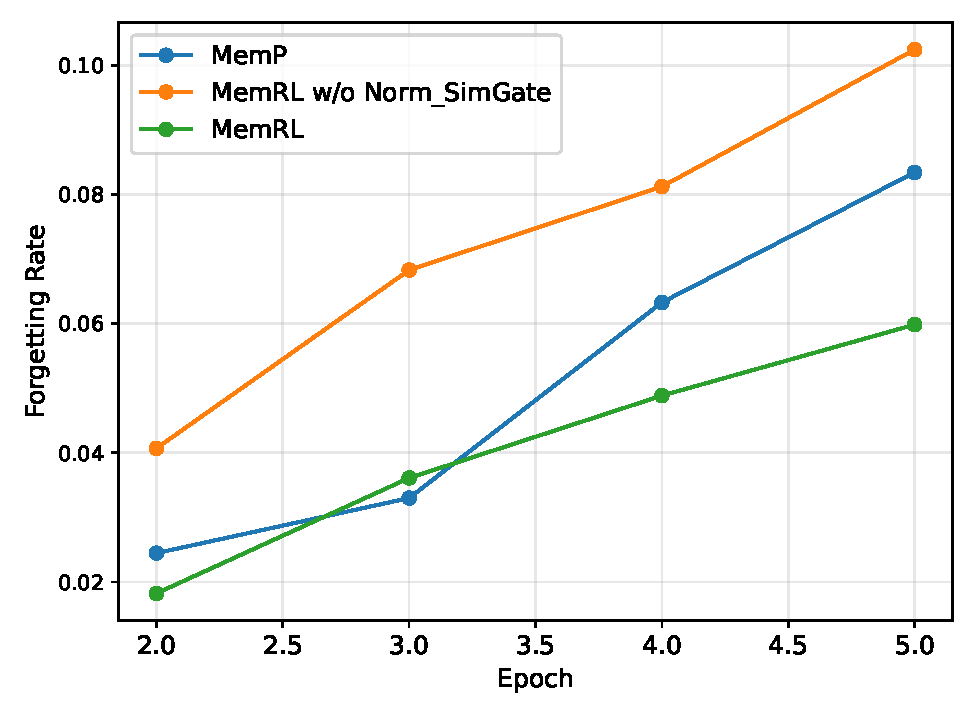
\includegraphics[width=\linewidth, height=5.0cm, keepaspectratio]{hle_forgetting_compare.pdf}
%     \caption{\textbf{Forgetting Rate in HLE.}}
%     \label{fig:transfer-forget}
%     \vspace{-0.15in}
% \end{figure}
% \begin{figure}[t]
%     \centering

%     % --- 子图 1 (上) ---
%     \begin{subfigure}{\linewidth}
%         \centering
%         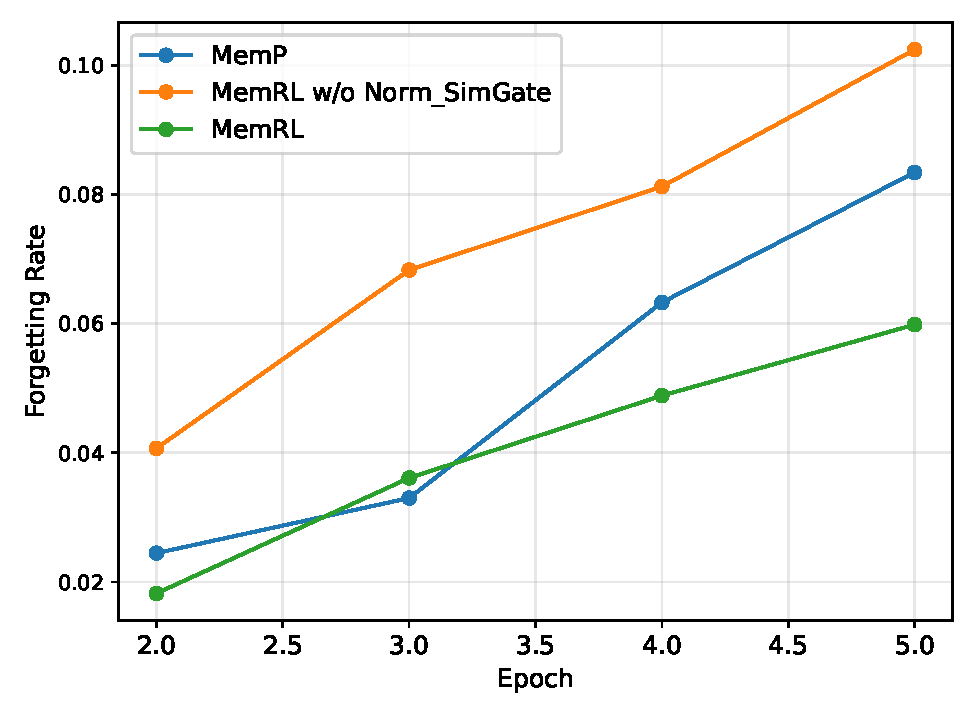
\includegraphics[width=\linewidth, height=5.0cm, keepaspectratio]{hle_forgetting_compare.pdf}
%         \caption{Forgetting Rate in HLE}
%         \label{fig:transfer-forget}
%     \end{subfigure}

%     \vspace{0.6em}

%     % --- 子图 2 (下) ---
%     \begin{subfigure}{\linewidth}
%         \centering
%         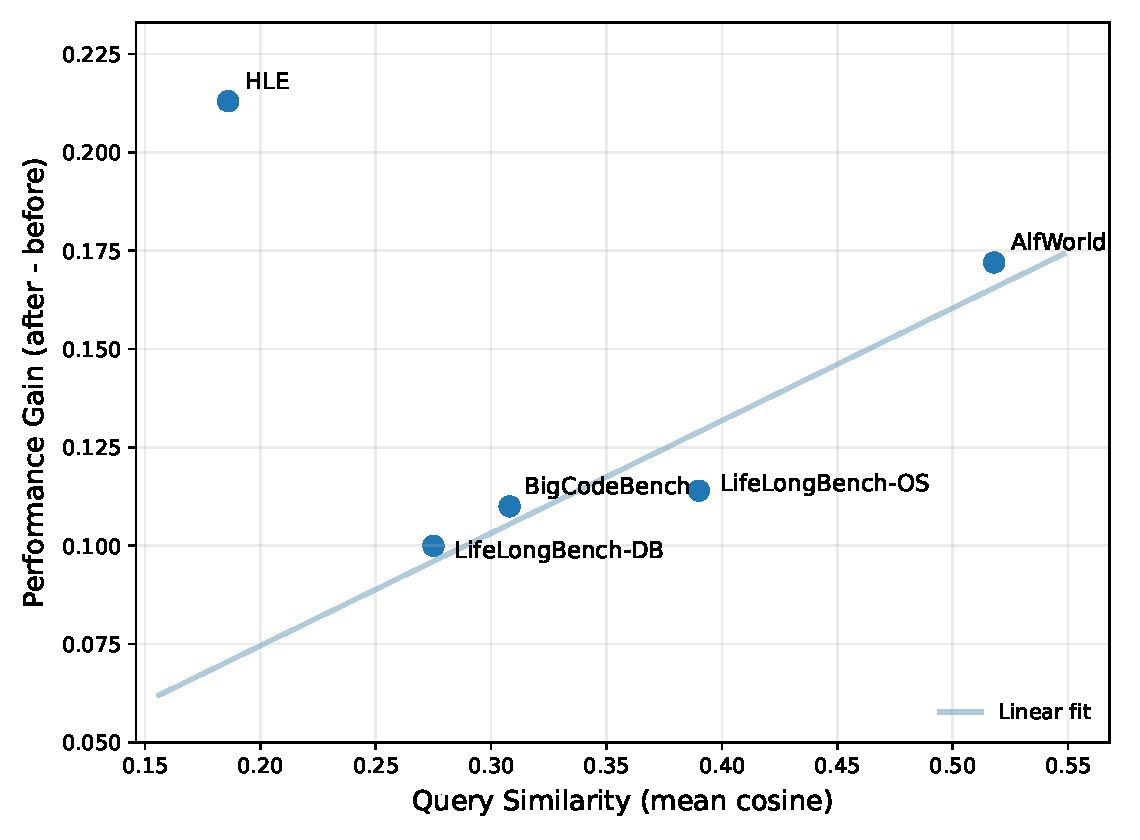
\includegraphics[width=\linewidth, height=5.0cm, keepaspectratio]{memory_generalization_vs_similarity.pdf}
%         \caption{Similarity-based Generalization}
%         \label{fig:sim_gain}
%     \end{subfigure}

%     \caption{\textbf{Forgetting and Generalization in HLE.}
%     (a) Forgetting rate comparison. (b) Similarity-based generalization analysis.}
%     \label{fig:forget_and_generalization}

%     \vspace{-0.15in}
% \end{figure}


% \subsubsection{Impact of Task Similarity on Memory Efficacy.}
% To understand the underlying conditions where \textsc{MemRL} thrives, we analyze the correlation between the intra-dataset semantic similarity ($\text{Sim}_{intra}$) and the absolute performance gain provided by our method ($\Delta = \text{Acc}_{\text{MemRL}} - \text{Acc}_{\text{NoMem}}$).

% As illustrated in Figure~\ref{fig:sim_gain}, we analyze the correlation between intra-dataset semantic similarity and the absolute performance gain ($\Delta$) provided by \textsc{MemRL}. The linear regression trend reveals a general positive correlation: environments with higher structural repetition allow the agent to retrieve and reuse optimal policies more effectively. At the upper extreme, \textbf{ALFWorld} (similarity $0.518$) acts as a strong anchor point for this trend, exhibiting the highest repetition and a corresponding maximum performance boost ($\Delta=+0.229$). This confirms that for highly repetitive procedural tasks, memory serves as an effective shortcut to optimal trajectories. Following the regression line, benchmarks with moderate similarity—such as \textbf{Lifelong-OS} ($0.390$) and \textbf{BigCodeBench} ($0.308$)—cluster in the middle region, showing steady improvements ($\Delta \approx +0.11 \sim +0.12$) where the agent successfully generalizes coding patterns or OS commands across related instructions.  

% \noindent \textbf{The HLE Anomaly: Generalization vs. Memorization.} 

% HLE presents a unique outlier. Despite having the lowest similarity ($0.186$) due to its diverse, multi-disciplinary nature, it exhibits a surprisingly high runtime gain ($0.357 \rightarrow 0.573, \Delta=+0.216$).   
% This gain operates on a different mechanism than ALFWorld. In high-similarity benchmarks, \textsc{MemRL} succeeds via \textit{Positive Transfer}—generalizing shared patterns to new instances. In contrast, the gain in HLE stems from \textit{Runtime Memorization}. Since HLE questions are distinct and domain-specific, the agent relies on the Runtime Learning phase to "memorize" specific solutions to difficult problems through repeated exposure. This distinction highlights \textsc{MemRL}'s versatility: it supports both \textit{pattern generalization} in structured domains and \textit{specific knowledge acquisition} in diverse domains.  

% 讨论记忆的质量与成功率的关系：记忆质量能够影响任务的成功率 讨论为什么RL有效

% \section{Limitation and Future Works}

% 多步MDP建模
% 意图聚类及慢更新
% 记忆的管理作为新的scaling维度，大脑记忆解耦的设想（模型只需要足够intelligent，不用过于knowledgable，进而探讨缩小模型参数量+增大记忆库的可能性）
\section{Limitations and Conclusion}

% \paragraph{Limitations and Future Work.}
% While \textsc{MemRL} establishes a foundation for non-parametric evolution, its runtime dynamics reveal several promising research avenues. (i) The current step-wise update, though fast, can introduce high-variance noise in long-horizon trajectories; multi-step slower updates or periodic memory consolidation could be explored. (ii) Credit-assignment ambiguity during multi-memory updates, especially with multiple referenced experiences, needs more precise attribution methods like Shapley values~\citep{shapley1953value} or value decomposition from multi-agent reinforcement learning. (iii) While \textsc{MemRL} excels with increasing task exposure, its performance can degrade towards reflection-like behavior when task similarity is low. This highlights the importance of maintaining a sufficient and varied experience base; for industrial deployment, strategies to ensure a high density of similar tasks or to facilitate hierarchical abstraction for generalization are crucial. Further detailed discussions on these and other challenges, including memory security, dedicated domains, and multi-agent memory sharing, are provided in Appendix~\ref{app:future_work}.

% \paragraph{Limitations and Future Work.}
% While \textsc{MemRL} establishes a foundation for non-parametric evolution, its runtime dynamics reveal several promising research avenues that we hope will provide insights for the community. Specifically, the current step-wise update protocol can introduce high-variance noise in long-horizon trajectories, identifying the stabilization of value estimation in extended sequences as a worthy direction for further study. Moreover, the credit-assignment ambiguity encountered during multi-memory updates suggests that achieving more precise experience attribution is a significant and open area for future research. By highlighting these subtle challenges, we aim to catalyze further innovation in value-aware agent architectures.
\paragraph{Limitations and Future Work.}
While \textsc{MemRL} establishes a foundation for non-parametric evolution, its runtime dynamics reveal several promising avenues. (i) The current step-wise update, though fast, may introduce high-variance noise in long-horizon trajectories, inspiring us to explore multi-step updates or periodic memory consolidation. (ii) Credit-assignment ambiguity during utility updates, especially with multiple referenced experiences, raises the need for more precise attribution methods like Shapley methods~\citep{shapley1953value} or value decomposition in multi-agent reinforcement learning~\citep{rashid2020monotonic,sunehag2017value}. (iii) While \textsc{MemRL} improves with increasing task exposure, performance may drift toward reflection-like behavior when task similarity is low, highlighting the need for a sufficiently diverse yet relevant experience base; for industrial deployment, ensuring high task density and hierarchical abstraction may be crucial. Further detailed discussions on these and other challenges, including memory security, dedicated domains, and multi-agent memory sharing, are provided in Appendix~\ref{app:future_work}.

\paragraph{Conclusion.}
We proposed \textsc{MemRL}, a non-parametric approach reconciling the stability-plasticity dilemma by treating memory retrieval as a value-based decision process. Through the Intent-Experience-Utility triplet structure and Monte Carlo style updates, \textsc{MemRL} enables agents to self-evolve and differentiate high-utility strategies from semantic noise without weight updates. Extensive evaluations confirm \textsc{MemRL} significantly outperforms baselines in both runtime adaptation and generalization. In a future where static training data becomes scarce, the interactive experiences generated by agents throughout their life cycle will become a new, vital source of knowledge. We hope this paradigm paves the way for building stable, continuously learning agents that efficiently adapt from interaction.
% \paragraph{Limitations.}
% Our runtime utility learning exhibits two distinct failure modes. \textbf{(i) Step-wise updates:} updating memory utilities at every interaction step injects high-variance noise into the value estimates, which can make utility rankings volatile—particularly for long-horizon trajectories with delayed or noisy outcome signals. \textbf{(ii) Multi-memory updates:} when several memories are retrieved for the same episode, applying the same outcome-level supervision to multiple items creates a credit-assignment ambiguity; the method has limited ability to separate causally useful experiences from incidental ones, potentially reinforcing spurious memories while under-crediting truly helpful ones. These issues can reduce the stability of Two-Phase Retrieval in heterogeneous deployment streams.

 % 单步更新不够稳定。每次都对检索到的memory更新q值会导致credit assignment分配不够清晰。

% 1. 单步更新速度快但方差较大不稳定，后续可以引入多步版本的慢更新，结合记忆中相似意图与经验的定期整合以进一步提高空间效率；
% 2. 多条被引用经验间的信用分配模糊问题，可以通过Shaply方法或者多智能体强化学习领域中的值分解方法进一步优化，提升算法的收敛效率；
% 3. 算法对reward hacking较为敏感，需要时刻注意验证器的false positive rate，因为一旦产生了fp样本，由于Q值的提高其错误的行为模式很可能被快速固化与传播。由此可以衍生出的挑战是记忆的安全性问题：即记忆库一旦被人为地注入攻击，其污染样本可能会快速扩散并导致智能体的系统性崩溃。因此在未来的研究中，智能体记忆的安全可信也会是一个非常重要的方向。不过幸好的是，由于经验的易于修改的特性，一旦定位到污染或者攻击，我们可以通过快速裁剪污染经验进行恢复，这并不会干扰到过往正常经验的效用。
% 4. 任务相似度不高时会退化为reflection，所以该方法见过的任务越多效果越好，不过这也符合Runtime Learning的特性。
% 并不是我们的方法效果不好，而是任务的特性问题（task和task太低）。增加任务相似度密度，对工业应用落地的建议。

% \section{Conclusion}

% In this paper, we introduced \textsc{MemRL}, a novel framework that enables LLMs to self-evolve through non-parametric reinforcement learning on episodic memory. Addressing the limitations of semantic retrieval and the instability of parameter fine-tuning, \textsc{MemRL} treats memory retrieval as a value-based decision process. By structuring memory into Intent-Experience-Utility triplets and applying Monte Carlo style updates, the agent learns to differentiate high-value strategies from semantic noise without modifying the backbone model weights.

% Our extensive evaluations across diverse domains—ranging from code generation to embodied navigation—demonstrate that \textsc{MemRL} significantly outperforms existing memory-augmented baselines in both runtime learning and generalization to unseen tasks. Theoretical and empirical analyses further reveal that \textsc{MemRL} effectively reconciles the stability-plasticity dilemma: the frozen LLM provides robust reasoning, while the evolving memory utility acts as a plastic channel for adaptation. Moreover, we identify that the utility-driven retrieval mechanism functions as a trajectory verifier, enabling the agent to filter out brittle policies in complex, multi-step tasks. We hope this work establishes a new paradigm for building self-evolving agents that can continuously learn from interaction in a stable and efficient manner.
\section*{Impact Statement}
This paper presents \textsc{MemRL}, a value-reinforced memory retrieval mechanism designed to enhance the long-term reasoning capabilities of LLM Agents. From a broader perspective, our work contributes to the development of more efficient and reliable autonomous systems. By optimizing the memory retrieval process, \textsc{MemRL} reduces the computational overhead of large-scale agent deployments, potentially lowering the environmental impact of AI infrastructure. Furthermore, as LLM agents become more integrated into daily workflows, research into robust memory mechanisms helps ensure these systems remain grounded and consistent in their actions. We do not foresee any immediate negative social consequences specific to this algorithmic advancement, though we acknowledge that all autonomous systems should be deployed with appropriate human oversight to mitigate broader risks associated with AI decision-making.


\bibliography{example_paper}
\bibliographystyle{icml2026}

%%%%%%%%%%%%%%%%%%%%%%%%%%%%%%%%%%%%%%%%%%%%%%%%%%%%%%%%%%%%%%%%%%%%%%%%%%%%%%%
%%%%%%%%%%%%%%%%%%%%%%%%%%%%%%%%%%%%%%%%%%%%%%%%%%%%%%%%%%%%%%%%%%%%%%%%%%%%%%%
% APPENDIX
%%%%%%%%%%%%%%%%%%%%%%%%%%%%%%%%%%%%%%%%%%%%%%%%%%%%%%%%%%%%%%%%%%%%%%%%%%%%%%%
%%%%%%%%%%%%%%%%%%%%%%%%%%%%%%%%%%%%%%%%%%%%%%%%%%%%%%%%%%%%%%%%%%%%%%%%%%%%%%%
% \newpage
% \appendix
% \onecolumn
% \section{You \emph{can} have an appendix here.}

% You can have as much text here as you want. The main body must be at most $8$
% pages long. For the final version, one more page can be added. If you want, you
% can use an appendix like this one.

% The $\mathtt{\backslash onecolumn}$ command above can be kept in place if you
% prefer a one-column appendix, or can be removed if you prefer a two-column
% appendix.  Apart from this possible change, the style (font size, spacing,
% margins, page numbering, etc.) should be kept the same as the main body.
%%%%%%%%%%%%%%%%%%%%%%%%%%%%%%%%%%%%%%%%%%%%%%%%%%%%%%%%%%%%%%%%%%%%%%%%%%%%%%%
%%%%%%%%%%%%%%%%%%%%%%%%%%%%%%%%%%%%%%%%%%%%%%%%%%%%%%%%%%%%%%%%%%%%%%%%%%%%%%%
% APPENDIX
%%%%%%%%%%%%%%%%%%%%%%%%%%%%%%%%%%%%%%%%%%%%%%%%%%%%%%%%%%%%%%%%%%%%%%%%%%%%%%%
%%%%%%%%%%%%%%%%%%%%%%%%%%%%%%%%%%%%%%%%%%%%%%%%%%%%%%%%%%%%%%%%%%%%%%%%%%%%%%%
\newpage
\onecolumn
\appendix
\raggedbottom


% ==========================================
% Appendix A: Theory
% ==========================================
\section{Theoretical Analysis and Proofs}
\label{app:theoretical_analysis}
\subsection{Stability Analysis}
\label{app:stability}

We analyze the stability of \textsc{MemRL} from a reinforcement learning perspective, focusing on the convergence behavior of the utility estimates stored in memory. \textsc{MemRL} performs non-parametric runtime learning using a constant-step-size update. We show that under mild and realistic assumptions, the learned utility values converge in expectation to stable estimates of memory effectiveness, with bounded variance.

\paragraph{Setup.}
At each time step $t$, the agent observes an intent state $s_t$, retrieves a memory item $m_t \in \mathcal{M}_t$, generates an output $a_t$, and receives a scalar reward $r_t \in [-1,1]$ indicating task success or failure. The generation policy follows the decomposition defined in Eq.~\ref{eq:joint_policy}, where $\mu$ denotes the retrieval policy and $p_{\mathrm{LLM}}$ is a frozen inference policy.

For each retrieved memory, \textsc{MemRL} updates its utility using the exponential moving average rule as formulated in Eq.~\ref{eq:q_update}, with learning rate $\alpha \in (0,1]$. For clarity in this analysis, we consider a fixed state--memory pair $(s,m)$ and write $Q_t \equiv Q_t(s,m)$.

\paragraph{Stationary Reward Assumption.}
We analyze the learning process on a fixed dataset and posit two key conditions that ensure the stability of the environment:
\begin{enumerate}
    \item \textbf{Frozen Inference Policy.} The parameters of $p_{\mathrm{LLM}}(y | s,m)$ and the evaluator's criteria are fixed.
    \item \textbf{Fixed Task Distribution.} Tasks $s$ are drawn from a stationary distribution over a fixed dataset.
\end{enumerate}
These assumptions guarantee that the learning target is well-defined: the expected reward for any specific task-memory pair is time-invariant. Thus, we have:
\begin{equation}
\mathbb{E}[r_t | s_t = s,\; m_t = m] = \beta(s,m).
\label{eq:stationary_reward}
\end{equation}

where the expectation is taken over the stochastic rewards resulting from the Inference Policy $p_{LLM}$ distribution.

\paragraph{Expected Convergence of Utility Estimates.}
We now state the main stability result.

\begin{theorem}
\label{thm:ema_convergence}
Let $\{Q_t\}$ be updated according to the rule in Eq.~\ref{eq:q_update} with constant step size $\alpha \in (0,1]$. If Eq.~\ref{eq:stationary_reward} holds and the pair $(s,m)$ is updated infinitely often, then:
\begin{equation}
\label{eq:sm-stable}
\lim_{t \to \infty} \mathbb{E}[Q_t] = \mathbb{E}[r_t | s_t = s,\; m_t = m] = \beta(s,m).
\end{equation}
Moreover, the convergence rate is exponential \citep{sutton2018reinforcement}:
\begin{equation}
\mathbb{E}[Q_t] - \beta(s,m)
=
(1-\alpha)^t\big(Q_0 - \beta(s,m)\big).
\end{equation}
\end{theorem}

\paragraph{Proof.}
Define the estimation error $e_t \triangleq Q_t - \beta(s,m)$. Based on the update rule in Eq.~\ref{eq:q_update}, the error recurrence relation is:
\begin{equation*}
e_{t+1}
=
(1-\alpha)e_t
+
\alpha\big(r_t - \beta(s,m)\big).
\end{equation*}
Taking conditional expectation given the history $\mathcal{F}_t$ and using Eq.~\ref{eq:stationary_reward}, we obtain:
\begin{equation*}
\mathbb{E}[e_{t+1} | \mathcal{F}_t]
=
(1-\alpha)e_t.
\end{equation*}
Taking full expectation yields:
\begin{equation*}
\mathbb{E}[e_{t+1}] = (1-\alpha)\mathbb{E}[e_t].
\end{equation*}
Iterating the recursion gives $\mathbb{E}[e_t] = (1-\alpha)^t e_0$, which converges to zero as $t \to \infty$. \hfill $\square$

We provide the detailed derivation of the convergence proof in Appendix~\ref{app:proof_convergence}.

\paragraph{Bounded Variance and Stability.}
If the reward variance $\mathrm{Var}(r_t | s,m) < \infty$, then the variance of $Q_t$ remains bounded:
\begin{equation}
\limsup_{t \to \infty} \mathrm{Var}(Q_t)
\le
\frac{\alpha}{2-\alpha}\,\mathrm{Var}(r_t | s,m).
\end{equation}
Thus, constant-step-size updates do not induce unbounded oscillations; instead, they yield stable utility estimates that track expected memory effectiveness while filtering high-frequency noise. We explicitly derive the variance bounds to demonstrate the global stability of the estimator under task clustering in Appendix~\ref{app:bounded_variance}.


\paragraph{Global Stability via EM Convergence.}
The stability of the local estimate (Theorem~\ref{thm:ema_convergence}) extends to the global memory utility $Q(m)$. By the linearity of expectation, $Q(m)$ acts as a Monte Carlo integrator striving to converge to:

\begin{equation}
\label{eq:global_convergence}
\lim_{t \to \infty} \mathbb{E}[Q_t(m)] 
= \mathbb{E}[r | m] 
= \sum_{s \in \mathcal{S}(m)} \underbrace{\mathbb{E}[r | s, m]}_{\text{Stationary}} \underbrace{\Pr(s | m)}_{\text{Retrieve-Dependent}}.
\end{equation}

where $\mathcal{S}(m) \triangleq \{ s \in \mathcal{S} | \text{sim}(s, z_m) \ge \tau_A \}$ denotes the \textit{effective support set} for memory $m$, comprising all task intents $s$ sufficiently similar to the memory's intent embedding $z_m$ to satisfy the Phase-A retrieval criterion.



A theoretical challenge arises here: the weighting term $\Pr(s | m)$ is a latent variable governed by the retrieval policy $\mu(m| s; \mathcal{M})$, which itself shifts as $Q$-values evolve. To prove convergence despite this dependency, we analyze \textsc{MemRL} as a \textbf{Generalized Expectation-Maximization (GEM)} process~\citep{dempster1977maximum, neal1998view}.
From a variational perspective, the system performs coordinate ascent on a global objective function $\mathcal{J}(Q, \mu)$ (the variational lower bound of expected reward):
(i) \textbf{E-Step (Policy Improvement):} The Phase-B ranking updates the retrieval policy $\mu$ to align with current estimates, monotonically increasing $\mathcal{J}$ with respect to $\mu$;
(ii) \textbf{M-Step (Value Update):} The utility update (Eq.~\ref{eq:q_update}) increases $\mathcal{J}$ with respect to $Q$.
By the \textit{Monotonic Improvement Theorem}~\citep{neal1998view}, this alternating optimization guarantees that the system converges to a stationary point where the retrieve policy stabilizes ($\mu_{t+1} \approx \mu_t$). Consequently, the induced distribution $\Pr(s | m)$ becomes time-invariant, ensuring that Eq.~\ref{eq:global_convergence} holds and effectively preventing catastrophic forgetting by anchoring updates to a stable policy. More details can be found in Appendix~\ref{app:gem_analysis}.


\subsection{Proof of Theorem~\ref{thm:ema_convergence}: Convergence of EMA Estimation}
\label{app:proof_convergence}

We aim to prove that for a fixed task-memory pair $(s,m)$ with a stationary reward distribution, the Q-value estimate $Q_t(s,m)$ converges in expectation to the true mean reward $\beta(s,m)$.

\paragraph{Assumptions.}
\begin{enumerate}[leftmargin=*]
    \item \textbf{Stationary Reward.} The reward $r_t$ at step $t$ is drawn from a distribution induced by the stochastic action generation $a \sim p_{LLM}(a_t | s_t, m)$, with a constant mean $\beta(s,m) = \mathbb{E}[r_t | s, m]$ and finite variance $\sigma^2$.
    \item \textbf{Update Rule.} The utility is updated via the linear EMA rule with learning rate $\alpha \in (0,1)$:
    \begin{equation*}
        Q_{t+1} = (1-\alpha)Q_t + \alpha r_t.
    \end{equation*}
\end{enumerate}

\paragraph{Derivation of Error Dynamics.}
Let $e_t \triangleq Q_t - \beta(s,m)$ be the estimation error at time step $t$. Substituting $Q_t = e_t + \beta(s,m)$ into the update rule:

\begin{align}
    e_{t+1} + \beta(s,m) &= (1-\alpha)(e_t + \beta(s,m)) + \alpha r_t \notag \\
    e_{t+1} &= (1-\alpha)e_t + (1-\alpha)\beta(s,m) + \alpha r_t - \beta(s,m) \notag \\
    e_{t+1} &= (1-\alpha)e_t + \beta(s,m) - \alpha\beta(s,m) - \beta(s,m) + \alpha r_t \notag \\
    e_{t+1} &= (1-\alpha)e_t + \alpha (r_t - \beta(s,m)). \label{eq:error_recurrence}
\end{align}

\paragraph{Convergence Analysis.}
We define $\mathcal{F}_t$ as the filtration (history) up to time $t$. Since the reward $r_t$ depends on the action $a_t$ sampled subsequently from the frozen LLM, taking the conditional expectation of Eq.~\ref{eq:error_recurrence} given $\mathcal{F}_t$:

\begin{equation*}
    \mathbb{E}[e_{t+1} | \mathcal{F}_t] = (1-\alpha)e_t + \alpha (\underbrace{\mathbb{E}[r_t | \mathcal{F}_t]}_{\beta(s,m)} - \beta(s,m)) = (1-\alpha)e_t.
\end{equation*}

By the Law of Iterated Expectations, taking the full expectation yields:
\begin{equation*}
    \mathbb{E}[e_{t+1}] = \mathbb{E}[\mathbb{E}[e_{t+1} | \mathcal{F}_t]] = (1-\alpha)\mathbb{E}[e_t].
\end{equation*}

Iterating this recurrence relation from $t=0$:
\begin{equation*}
    \mathbb{E}[e_t] = (1-\alpha)^t \mathbb{E}[e_0].
\end{equation*}

Since $0 < \alpha < 1$, we have $|1-\alpha| < 1$. Consequently:
\begin{equation}
    \lim_{t \to \infty} \mathbb{E}[e_t] = \mathbb{E}[e_0] \cdot \lim_{t \to \infty} (1-\alpha)^t = 0.
\end{equation}

This proves that the estimator is unbiased in the limit, i.e., $\lim_{t \to \infty} \mathbb{E}[Q_t] = \beta(s,m)$. \hfill $\square$


\subsection{Bounded Variance and Global Stability}
\label{app:bounded_variance}

In this section, we provide the formal derivation for the variance bound of the estimator $Q_t$. We explicitly derive the finite-time variance formula via recursive unrolling and prove its asymptotic convergence, demonstrating how Phase-A clustering contributes to global stability.

\paragraph{Derivation of the Variance Bound.}
Let $\sigma^2 \triangleq \mathrm{Var}(r_t | s, m)$ be the variance of the reward signal, assumed to be finite. The EMA update rule is given by:
\begin{equation*}
    Q_{t+1} = (1-\alpha)Q_t + \alpha r_t.
\end{equation*}
Since the reward $r_t$ (current noise) is statistically independent of the current estimate $Q_t$ (which is determined by history $\mathcal{F}_{t-1}$), the variance of the sum is the sum of the variances:
\begin{align*}
    \mathrm{Var}(Q_{t+1}) 
    &= \mathrm{Var}((1-\alpha)Q_t) + \mathrm{Var}(\alpha r_t) \\
    &= (1-\alpha)^2 \mathrm{Var}(Q_t) + \alpha^2 \sigma^2.
\end{align*}
Let $v_t \triangleq \mathrm{Var}(Q_t)$. We obtain a linear recurrence relation $v_{t+1} = (1-\alpha)^2 v_t + \alpha^2 \sigma^2$.

\paragraph{Recursive Unrolling.}
To solve for $v_t$, we expand the recurrence relation backward from step $t$:
\begin{align}
    v_t &= (1-\alpha)^2 v_{t-1} + \alpha^2 \sigma^2 \notag \\
    &= (1-\alpha)^2 \left[ (1-\alpha)^2 v_{t-2} + \alpha^2 \sigma^2 \right] + \alpha^2 \sigma^2 \notag \\
    &= (1-\alpha)^4 v_{t-2} + \alpha^2 \sigma^2 \left[ 1 + (1-\alpha)^2 \right] \notag \\
    &\quad \vdots \nonumber \\
    &= (1-\alpha)^{2t} v_0 + \alpha^2 \sigma^2 \sum_{k=0}^{t-1} \left( (1-\alpha)^2 \right)^k. \label{eq:variance_summation}
\end{align}
Eq.~\ref{eq:variance_summation} explicitly shows that the variance at time $t$ consists of two components: the decayed initial variance (first term) and the accumulated noise variance (second term).

\paragraph{Asymptotic Convergence.}
As $t \to \infty$, since the learning rate $\alpha \in (0,1)$, the term $(1-\alpha)^{2t}$ vanishes. The summation term is a geometric series $\sum_{k=0}^{\infty} r^k = \frac{1}{1-r}$ with ratio $r = (1-\alpha)^2$. Thus:
\begin{equation*}
    \lim_{t \to \infty} v_t 
    = \alpha^2 \sigma^2 \cdot \frac{1}{1 - (1-\alpha)^2}.
\end{equation*}
Evaluating the denominator:
\begin{equation*}
    1 - (1-\alpha)^2 = 1 - (1 - 2\alpha + \alpha^2) = 2\alpha - \alpha^2 = \alpha(2-\alpha).
\end{equation*}
Substituting this back yields the tight variance bound:
\begin{equation}
    \limsup_{t \to \infty} \mathrm{Var}(Q_t) 
    = \frac{\alpha^2 \sigma^2}{\alpha(2-\alpha)} 
    = \frac{\alpha}{2-\alpha} \sigma^2.
\end{equation}

\paragraph{Connection to Phase-A Clustering.}
This result provides the theoretical justification for the stability of \textsc{MemRL}. While tasks within a memory cluster $\mathcal{S}(m) \triangleq \{ s | \text{sim}(s, z_m) > \tau_A \}$ may vary, the Smoothness Assumption implies their rewards are drawn from a distribution with bounded variance $\sigma^2_{\mathcal{S}(m)}$.
The derived bound $\frac{\alpha}{2-\alpha} \sigma^2_{\mathcal{S}(m)}$ guarantees that the memory utility $Q(m)$ will not diverge but will instead oscillate within a controlled range around the true expected utility. This mechanism effectively filters out high-frequency noise from diverse task instances while retaining the stable generalized value.

\subsection{Convergence via Variational Inference}
\label{app:gem_analysis}

In this section, we provide a theoretical foundation for \textsc{MemRL}, demonstrating that our retrieval strategy and update rules guarantee the convergence of value estimation.

\subsubsection{The Convergence Objective}
Our ultimate goal is to ensure that the estimated utility $Q(m)$ converges to the true expected return of memory $m$. This target value is defined as:
\begin{equation}
\label{eq:global_convergence2}
\lim_{t \to \infty} \mathbb{E}[Q_t(m)] 
= \mathbb{E}[r | m] 
= \sum_{s \in \mathcal{S}(m)} \underbrace{\mathbb{E}[r | s, m]}_{\text{Stationary}} \underbrace{\Pr(s | m)}_{\text{Retrieve-Dependent}}.
\end{equation}
The challenge lies in the term $\Pr(s | m)$—the probability that a specific state $s$ triggers the retrieval of $m$. This distribution depends on the retrieval policy $\mu_t(m|s)$, which itself evolves during training, creating a circular dependency that threatens stability.

\subsubsection{Variational Objective with Trust Region}
To resolve this, we formulate the problem as maximizing a \textbf{global variational objective} $\mathcal{J}(\mu, Q)$. This objective serves as a tractable lower bound for the global expected return defined in Eq.~\ref{eq:global_convergence2}, balanced by a semantic trust region:
\begin{equation}
\label{eq:variational_objective}
\mathcal{J}(\mu, Q) = \mathbb{E}_{s \sim \mathcal{D}} \left[ \underbrace{\sum_{m \in \mathcal{S}(s)} \mu(m|s) Q(s, m)}_{\text{Expected Utility } \approx \mathbb{E}[Q_t(m)]} - \frac{1}{\beta} \underbrace{D_{\text{KL}}\Big(\mu(\cdot|s) \big\| \pi_{\text{sim}}(\cdot|s)\Big)}_{\text{Semantic Trust Region}} \right]
\end{equation}
Here, the expectation is taken over the state distribution $\mathcal{D}$. The first term directly corresponds to the expected utility $\mathbb{E}[Q_t(m)]$ we aim to converge, while $\pi_{\text{sim}}$ represents the fixed semantic prior (derived from Phase-A). The KL-divergence term acts as a regularizer crucial for two reasons:
\begin{enumerate}[leftmargin=*]
    \item \textbf{Trust Region:} It constrains the policy to the support set $\mathcal{S}$, preventing the agent from retrieving high-Q but semantically irrelevant memories (out-of-distribution errors).
    \item \textbf{Regularization:} It stabilizes the learning dynamics during the ``cold start'' phase when Q-estimates are noisy.
\end{enumerate}

\subsubsection{Optimization via Generalized Expectation-Maximization (GEM)}
We treat the optimization of $\mathcal{J}$ as a GEM process, alternating between policy improvement and value evaluation:

\paragraph{E-Step (Policy Optimization).} 
We assume the utility estimates $Q(s, m)$ are fixed and seek the optimal retrieval policy $\mu^*$ that maximizes the global variational objective $\mathcal{J}(\mu, Q)$. Since the expectation is taken over the state distribution $\mathcal{D}$, we can maximize the objective for each state $s$ pointwise. The optimization problem for a specific state $s$ is:

\begin{equation}
\max_{\mu(\cdot|s)} \left[ \sum_{m \in \mathcal{S}(s)} \mu(m|s) Q(s, m) - \frac{1}{\beta} D_{\text{KL}}\Big(\mu(\cdot|s) \big\| \pi_{\text{sim}}(\cdot|s)\Big) \right]
\end{equation}
subject to the probability simplex constraint $\sum_{m \in \mathcal{S}(s)} \mu(m|s) = 1$.

Expanding the KL-divergence term, the objective function becomes:
\begin{equation}
\mathcal{L}(\mu) = \sum_{m \in \mathcal{S}(s)} \mu(m|s) \left( Q(s, m) + \frac{1}{\beta} \log \frac{\pi_{\text{sim}}(m|s)}{\mu(m|s)} \right).
\end{equation}

To enforce the normalization constraint, we introduce the Lagrange multiplier $\lambda$ and construct the Lagrangian:
\begin{equation*}
L(\mu, \lambda) = \sum_{m \in \mathcal{S}(s)} \mu(m|s) \left( Q(s, m) + \frac{1}{\beta} \log \frac{\pi_{\text{sim}}(m|s)}{\mu(m|s)} \right) + \lambda \left( 1 - \sum_{m \in \mathcal{S}(s)} \mu(m|s) \right).
\end{equation*}

Taking the derivative with respect to $\mu(m|s)$ and setting it to zero:
\begin{equation*}
\begin{aligned}
\frac{\partial L}{\partial \mu(m|s)} &= Q(s, m) + \frac{1}{\beta} \left( \log \frac{\pi_{\text{sim}}(m|s)}{\mu(m|s)} + \mu(m|s) \cdot \frac{\mu(m|s)}{\pi_{\text{sim}}(m|s)} \cdot \frac{-\pi_{\text{sim}}(m|s)}{\mu(m|s)^2} \right) - \lambda \\
&= Q(s, m) + \frac{1}{\beta} \left( \log \frac{\pi_{\text{sim}}(m|s)}{\mu(m|s)} - 1 \right) - \lambda = 0.
\end{aligned}
\end{equation*}

Rearranging terms to solve for $\mu(m|s)$:
\begin{equation*}
\begin{aligned}
\log \frac{\pi_{\text{sim}}(m|s)}{\mu(m|s)} &= \beta \lambda - \beta Q(s, m) + 1 \\
\frac{\mu(m|s)}{\pi_{\text{sim}}(m|s)} &= \exp\left( \beta Q(s, m) - (\beta \lambda + 1) \right) \\
\mu(m|s) &= \pi_{\text{sim}}(m|s) \exp(\beta Q(s, m)) \cdot \exp(-(\beta \lambda + 1)).
\end{aligned}
\end{equation*}

Since $\exp(-(\beta \lambda + 1))$ is independent of $m$, it acts as a normalization constant $1/Z(s)$. Thus, we recover the closed-form Boltzmann distribution used in our Phase-B retrieval:
\begin{equation*}
\mu^*(m|s) = \frac{\pi_{\text{sim}}(m|s) \exp(\beta Q(s, m))}{Z(s)} \propto \pi_{\text{sim}}(m|s) \exp(\beta Q(s, m)).
\end{equation*}
This derivation theoretically justifies our heuristic scoring function: the optimal retrieval policy naturally balances the semantic prior $\pi_{\text{sim}}$ and the learned utility $Q$.
By taking the logarithm, we recover the specific scoring function used in our \textbf{Phase-B Retrieval} (Eq.~\ref{eq:score}):
\begin{equation*}
\log \mu^*(m|s) \propto \underbrace{\log \pi_{\text{sim}}(m|s)}_{\approx \text{sim}(s, m)} + \beta Q_t(s, m)
\end{equation*}
This proves that our heuristic combination of similarity and Q-value is mathematically equivalent to the optimal policy under the variational objective.

\paragraph{M-Step (Policy Evaluation via Error Minimization).} 
While the E-step improves the policy based on current estimates, the M-step ensures these estimates are grounded in reality. Fixing the policy $\mu_{t+1}$, our goal is to align the variational parameter $Q$ with the true environmental returns. We formulate this as minimizing the Mean Squared Error (MSE) between the estimated utility and the observed reward target $y = r$ (in our Monte Carlo style modeling):
\begin{equation}
\min_Q \mathcal{L}(Q) = \mathbb{E}_{\tau \sim \mu_{t+1}} \left[ \frac{1}{2} \left( y - Q(s, m) \right)^2 \right]
\end{equation}
Minimizing this error is critical because it tightens the variational bound: it ensures that the expectation term $\mathbb{E}[Q]$ in the global objective $\mathcal{J}$ (Eq.~\ref{eq:variational_objective}) converges to the true expected return $\mathbb{E}[r]$.
The update rule used in our approach (Eq.~\ref{eq:q_update}) corresponds exactly to a Stochastic Gradient Descent (SGD) step on this objective:
\begin{equation*}
Q_{t+1}(s, m) \leftarrow Q_t(s, m) - \alpha \nabla_Q \mathcal{L}(Q) = Q_t(s, m) + \alpha (y - Q_t(s, m))
\end{equation*}
By iteratively minimizing $\mathcal{L}(Q)$, the M-step propagates the environmental feedback into the utility estimates, ensuring that the subsequent E-step optimization occurs on a reliable value landscape.

\subsubsection{Proof of Convergence}
By the \textit{Monotonic Improvement Theorem} of GEM~\citep{neal1998view}, the sequence $(\mu_t, Q_t)$ is guaranteed to converge to a stationary point $(\mu^*, Q^*)$.
At stationarity, the policy stabilizes ($\mu_{t+1} \approx \mu_t$), which implies that the inverse retrieval probability $\Pr(s|m)$ becomes \textbf{time-invariant}:
\begin{equation*}
\Pr(s|m) = \frac{\mu^*(m|s)\Pr(s)}{\sum_{s'} \mu^*(m|s')\Pr(s')}
\end{equation*}
Consequently, the ``Retrieve-Dependent'' term in Eq.~\ref{eq:global_convergence2} is anchored. With a fixed data distribution, the  $Q_t(m)$ converges to the unique fixed point:
\begin{equation}
\lim_{t \to \infty} Q_t(m) \to \mathbb{E}_{\mu^*}[r | m]
\end{equation}
Thus, our approach theoretically guarantees that the memory values converge to the true expected returns under the optimal retrieval policy.

% ==========================================
% Appendix B: Implementation
% ==========================================

\section{Extended Analysis and Insights}
\label{app:analysis}

\subsection{Detailed Analysis of Forgetting Dynamics}
\label{app:forgetting_dynamics}

In the main text, we reported the mean forgetting rate to quantify the stability of our method. Here, we provide a detailed visual analysis of how the forgetting rate evolves throughout the learning process on the HLE benchmark.

\begin{figure}[h] % 建议在附录里用 h 或 t
    \centering
    % 确保你的文件路径是正确的
    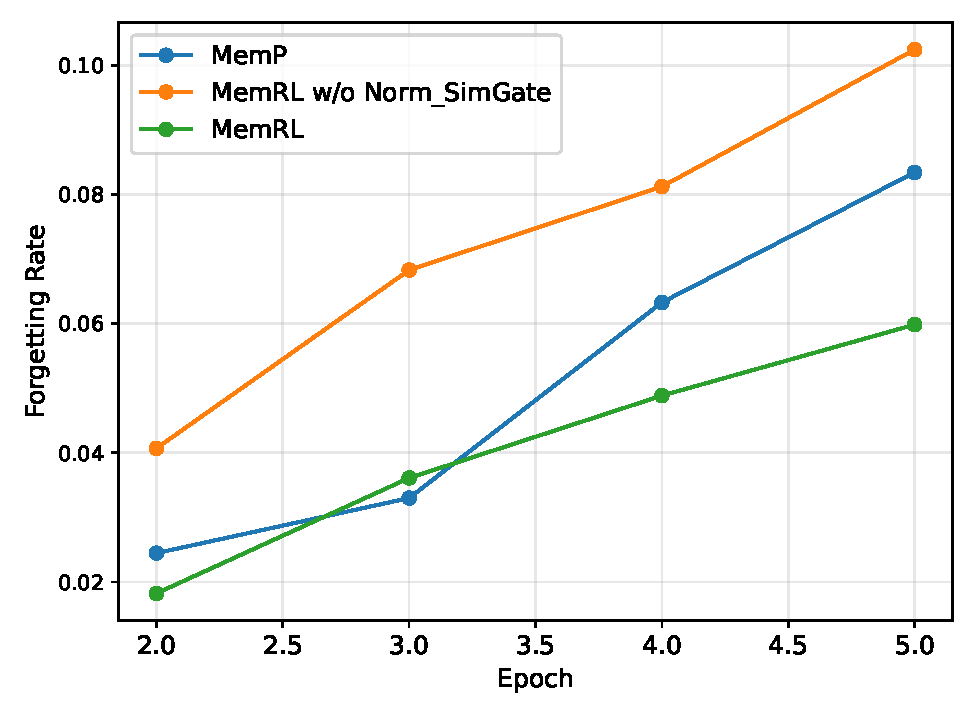
\includegraphics[width=0.5\linewidth]{hle_forgetting_compare.pdf}
    \caption{\textbf{Forgetting Rate Trajectory on HLE.} We compare the cumulative forgetting rate of the \textsc{MemRL} against the strong baseline MemP and an ablated version of \textsc{MemRL} (w/o Normalization \& Gating). A lower curve indicates better stability (less catastrophic forgetting).}
    \label{fig:transfer-forget}
\end{figure}

As illustrated in Figure~\ref{fig:transfer-forget}, \textsc{MemRL} demonstrates superior stability compared to MemP. Specifically:
\begin{itemize}
    \item \textbf{Stability vs. Plasticity:} While MemP shows a gradual upward trend in forgetting rate as the number of episodes increases, \textsc{MemRL} maintains a consistently low rate. This indicates that our dual-retrieval mechanism effectively balances the acquisition of new strategies without overwriting stable, high-utility memories.
    
    \item \textbf{Impact of Filtering:} The ablation curve (denoted as \textit{w/o Norm \& SimGate}) exhibits significant higher overall forgetting rate ($0.073$ mean). The visible spikes in the curve suggest that without z-score normalization and similarity gating, the agent frequently retrieves and reinforces ``noisy" strategies that work for specific instances but degrade general performance on previously mastered tasks.
\end{itemize}

\subsection{\textsc{MemRL} as a Trajectory Verifier.}

% --- 文字环绕开始 ---
% 宽度设为 0.6\textwidth 以容纳 "BigCodeBench" 这种长词
% \begin{wraptable}{r}{0.6\textwidth}
%     \vspace{-0.25in} % 对齐第一行文字
%     \centering
%     \footnotesize  % 改用 footnotesize 保证长词能放下
%     \setlength{\tabcolsep}{1.5pt} % 稍微收紧列间距
    
%     \caption{\textbf{Impact of Task Structure.} Comparison of Cumulative Success Rate (CSR) gains. Multi-step tasks benefit significantly more from MemRL.}
%     \label{tab:horizon_analysis}
    
%     \begin{tabular}{@{}l l c c c@{}}
%         \toprule
%         \textbf{Benchmark} & \textbf{Interaction} & \textbf{MemP} & \textbf{MemRL} & \textbf{Gain} \\
%         & & \textbf{(\%)} & \textbf{(\%)} & \textbf{(pp)} \\
%         \midrule
%         ALFWorld     & Multi-step  & 45.6 & \textbf{69.7} & \textbf{+24.1} \\
%         OS Task      & Multi-step  & 74.3 & \textbf{81.7} & \textbf{+7.4}  \\
%         HLE          & Single-step & 58.2 & 61.3 & +3.1 \\
%         BigCodeBench & Single-step & 60.2 & 62.7 & +2.5 \\
%         \bottomrule
%     \end{tabular}
%     \vspace{-0.1in}
% \end{wraptable}
\begin{table}[h]  % t / h / b / H 按需要调
    \centering
    \footnotesize
    \setlength{\tabcolsep}{1.5pt}

    \caption{\textbf{Impact of Task Structure.} Comparison of Cumulative Success Rate (CSR) gains. Multi-step tasks benefit significantly more from \textsc{MemRL}.}
    \label{tab:horizon_analysis}

    \begin{tabular}{@{}l l c c c@{}}
        \toprule
        \textbf{Benchmark} & \textbf{Interaction} & \textbf{MemP (\%)} & \textbf{\textsc{MemRL} (\%)} & \textbf{Gain (pp)} \\
        % & & \textbf{(\%)} & \textbf{(\%)} & \textbf{(pp)} \\
        \midrule
        ALFWorld     & Multi-step  & 91.9 & \textbf{98.1} & \textbf{+6.2} \\
        OS Task      & Multi-step  & 74.2 & \textbf{80.4} & \textbf{+6.2}  \\
        HLE          & Single-step & 57.0 & 60.6 & +3.6 \\
        BigCodeBench & Single-step & 60.2 & 62.7 & +2.5 \\
        \bottomrule
    \end{tabular}
\vskip -5pt
\end{table}
% --- 表格结束 ---

Table~\ref{tab:horizon_analysis} reveals a correlation between task structural complexity and performance gain. The gains are most profound in multi-step sequential tasks (e.g., ALFWorld $+6.2\%$ Points(pp)) compared to single-turn tasks (e.g., BigCodeBench $+2.5\%$ pp).
In sequential tasks, a retrieved memory must be valid for the \textit{entire} trajectory. Standard semantic retrieval often fetches memories that match the initial instruction but fail in later steps. By propagating the final reward backward to the memory utility $Q$, \textsc{MemRL} effectively learns to verify the \textit{whole trajectory}, filtering out brittle policies that look correct only on the surface.

This analysis indicates that \textsc{MemRL} transcends the role of a simple retrieval enhancer to function as a \textit{Trajectory Verifier}. Its value is maximized in tasks with complex temporal dependencies, where it learns to select memories that ensure the structural integrity of the entire interaction process.

\subsection{Impact of Task Similarity on Memory Efficacy}
\label{app:sim-analysis}
To understand the underlying conditions where \textsc{MemRL} thrives, we analyze the correlation between the intra-dataset semantic similarity ($\text{Sim}_{intra}$) and the absolute performance gain provided by our method ($\Delta = \text{Success Rate}_{\text{MemRL}} - \text{Success Rate}_{\text{NoMem}}$).
    \begin{figure}[H]
    \centering
    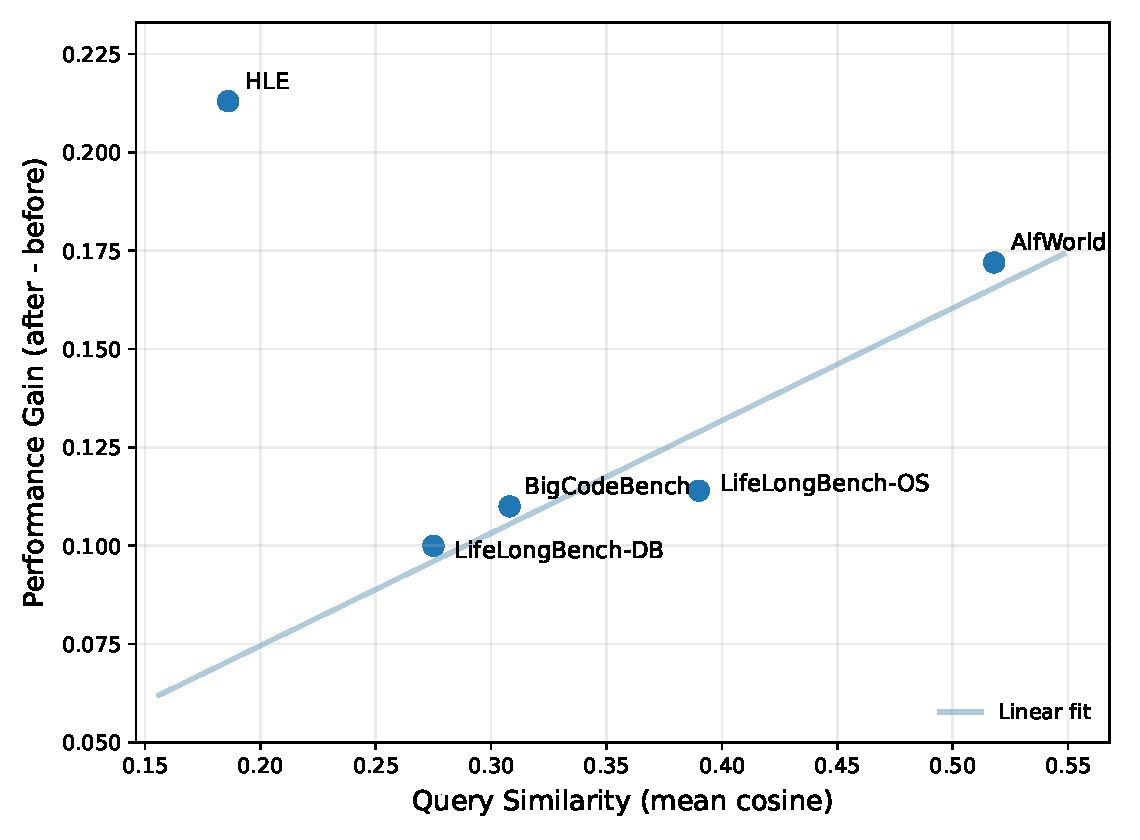
\includegraphics[width=0.4\linewidth]{memory_generalization_vs_similarity.pdf}
    \caption{\textbf{Similarity-based Generalization.}}
    \label{fig:sim_gain}
\end{figure}
As illustrated in Figure~\ref{fig:sim_gain}, we analyze the correlation between intra-dataset semantic similarity and the absolute performance gain ($\Delta$) provided by \textsc{MemRL}. The linear regression trend reveals a general positive correlation: environments with higher structural repetition allow the agent to retrieve and reuse optimal policies more effectively. At the upper extreme, \textbf{ALFWorld} (similarity $0.518$) acts as a strong anchor point for this trend, exhibiting the highest repetition and a corresponding maximum performance boost ($\Delta=+0.172$). This confirms that for highly repetitive procedural tasks, memory serves as an effective shortcut to optimal trajectories. Following the regression line, benchmarks with moderate similarity—such as \textbf{Lifelong-OS} ($0.390$) and \textbf{BigCodeBench} ($0.308$)—cluster in the middle region, showing steady improvements ($\Delta \approx +0.10 \sim +0.11$) where the agent successfully generalizes coding patterns or OS commands across related instructions.  

\noindent \textbf{The HLE Anomaly: Generalization vs. Memorization.} 

HLE presents a unique outlier. Despite having the lowest similarity ($0.186$) due to its diverse, multi-disciplinary nature, it exhibits a surprisingly high runtime gain ($0.357 \rightarrow 0.570, \Delta=+0.213$).   
This gain operates on a different mechanism than ALFWorld. In high-similarity benchmarks, \textsc{MemRL} succeeds via \textit{Positive Transfer}—generalizing shared patterns to new instances. In contrast, the gain in HLE stems from \textit{Runtime Memorization}. Since HLE questions are distinct and domain-specific, the agent relies on the Runtime Learning phase to ``memorize" specific solutions to difficult problems through repeated exposure. This distinction highlights \textsc{MemRL}'s versatility: it supports both \textit{pattern generalization} in structured domains and \textit{specific knowledge acquisition} in diverse domains.  

% ==========================================
% Appendix E: New Experiments (Transfer & Merging)
% ==========================================
\section{Advanced Capabilities: Transfer and Merging}
\label{app:advanced_exp}
\subsection{Cross-Model Memory Transferability}
\label{app:memory_transfer}

We investigate whether the procedural knowledge captured by \textsc{MemRL} is specific to the training policy or if it generalizes across different architectures. To test this, we take a memory bank fully trained for 10 epochs on the HLE benchmark using our strongest agent, \texttt{Gemini-3-pro}, and directly transfer it—without any fine-tuning—to three distinct inference models: \texttt{Qwen3-235B}, \texttt{GPT-5.2(High)}, and \texttt{Gemini-3-flash}.

As summarized in Table~\ref{tab:transfer_models}, the transferred memory yields substantial zero-shot performance gains across all models. Notably, smaller or distilled models experience the largest relative improvements; for instance, \texttt{Qwen3-235B} improves by over $3\times$ ($0.150 \rightarrow 0.531$) and \texttt{Gemini-3-flash} nearly doubles its success rate ($0.347 \rightarrow 0.583$). Even \texttt{GPT-5.2(High)}, a highly capable reasoning model, sees a significant boost ($0.354 \rightarrow 0.571$). 

These results suggest that \textsc{MemRL} captures \textit{model-agnostic} problem-solving patterns—such as efficient code skeletons and reasoning templates—rather than model-specific artifacts. This effectively allows the memory bank to function as a portable knowledge base, enabling weaker models to ``inherit" the capabilities of a stronger teacher model through simple retrieval.

\begin{table}[h]
\centering
\caption{\textbf{Cross-Model Transfer Results on HLE.} Performance of various agents using a frozen memory bank originally trained by \texttt{Gemini-3-pro}. $\Delta$ denotes the absolute improvement over the base model.}
\label{tab:transfer_models}
\resizebox{0.6\linewidth}{!}{%
\begin{tabular}{l c c c}
\toprule
\textbf{Inference Model} & \textbf{Base Score} & \textbf{Transfer Score} & \textbf{Gain ($\Delta$)} \\
\midrule
\texttt{Qwen3-235B} & 0.150 & 0.531 & \textbf{+0.381} \\
\texttt{Gemini-3-flash} & 0.347 & 0.583 & +0.236 \\
\texttt{GPT-5.2(High)} & 0.354 & 0.571 & +0.217 \\
\bottomrule
\end{tabular}%
}
\end{table}


\subsection{Multi-Task Memory Merging and Interference Analysis}
To evaluate the composability and robustness of \textsc{MemRL} in multi-task scenarios, we conducted a memory merging experiment. Specifically, we aggregated the finalized memory banks learned from the last epoch of two distinct domains within the Lifelong Agent Bench: Operating System Control ($M_{OS}$) and Database Management ($M_{DB}$). The agent was then evaluated on each respective benchmark using this unified, heterogeneous memory bank ($M_{Unified} = M_{OS} \cup M_{DB}$), without any further training or fine-tuning.

As presented in Table \ref{tab:memory_merge}, the results demonstrate that merging memories introduces negligible interference. The performance on the DB Task remains identical ($0.960$), while the OS Task exhibits only a marginal fluctuation ($0.788 \rightarrow 0.784$). This robustness is intrinsic to our \textbf{Two-Phase Retrieval} mechanism. Since the semantic spaces of OS commands and SQL queries are largely orthogonal, the Phase-A similarity filter effectively acts as a semantic gate, automatically excluding irrelevant cross-task memories before they enter the value-based ranking stage. This confirms that \textsc{MemRL} supports modular memory composition, allowing agents to scale capabilities by simply merging memory modules without suffering from negative transfer or catastrophic interference.

\begin{table}[H]
    \centering
    \small
    \caption{\textbf{Memory Merging Results.} Performance comparison between using task-specific individual memory banks versus a merged unified memory bank. The minimal delta confirms strong resistance to cross-task interference.}
    \label{tab:memory_merge}
    \setlength{\tabcolsep}{8pt}
    \begin{tabular}{l c c c}
        \toprule
        \textbf{Benchmark Task} & \textbf{Individual Memory} & \textbf{Merged Memory} & \textbf{Performance Delta} \\
        & (Original) & ($M_{OS} \cup M_{DB}$) & ($\Delta$) \\
        \midrule
        Lifelong-OS (OS Task) & 0.788 & 0.784 & -0.004 \\
        Lifelong-DB (DB Task) & 0.960 & 0.960 & \phantom{-}0.000 \\
        \bottomrule
    \end{tabular}
\end{table}

\section{Baseline and Benchmark Details}
\label{app:baseline_benchmark_details}

To ensure a rigorous evaluation, we compare \textsc{MemRL} against a diverse set of baselines ranging from simple sampling strategies to advanced agentic memory systems. All baselines are evaluated under a \textbf{unified frozen-backbone setting} to isolate the contribution of the memory and retrieval mechanisms.

\subsection{Baselines}
\label{app:baselines}
We categorize the baselines into three groups based on their interaction with memory and environment:

\paragraph{I. Test-Time Scaling Strategy}
\begin{itemize}
    \item \textbf{Pass@k:} This is a standard sampling-based baseline. It generates $k$ independent candidate solutions for a given query and selects the best one based on the benchmark's verifier (if available) or reports the success rate if at least one candidate passes. This baseline serves as a measure of the inherent capability of the frozen LLM without any memory persistence.
\end{itemize}

\paragraph{II. Retrieval-Augmented Generation (RAG) Approaches}
\begin{itemize}
    \item \textbf{RAG \citep{lewis2020retrieval}:} Represents the standard semantic retrieval paradigm. It utilizes an embedding model to encode the current query and retrieves the top-$k$ most semantically similar past experiences (or documents) from the external memory. These retrieved contexts are then prepended to the prompt to guide the LLM's generation.
    
    \item \textbf{Self-RAG \citep{asai2023selfrag}:} An advanced RAG variant that incorporates a self-critique mechanism. Unlike standard RAG, Self-RAG performs selective retrieval and uses a critique model (or self-prompting) to verify the relevance and factual correctness of the retrieved content before integrating it into the generation process.
\end{itemize}

\paragraph{III. Agentic Memory Systems}
\begin{itemize}
    \item \textbf{Mem0 \citep{chhikara2025mem0}:} A recently proposed memory layer for LLMs that manages memory through structured operations. It employs specific APIs for adding, retrieving, and updating memory, aiming to maintain a personalized and persistent context across interactions.
    
    \item \textbf{MemP \citep{fang2025memp}:} A framework focused on procedural memory. It distills past successful trajectories into reusable, procedure-like memory entries. MemP maintains a memory repository using a build-retrieve-update cycle, allowing the agent to recall high-level plans rather than raw trajectory data.
\end{itemize}

\subsection{Benchmark Datasets}
\label{app:benchmark}
We evaluate performance across four benchmarks selected to cover diverse domains: code generation, OS interactions, embodied decision-making, and multidisciplinary reasoning.

\begin{itemize}
    \item \textbf{BigCodeBench \citep{zhuo2025bigcode}:} A challenging benchmark for library-oriented code generation that requires agents to implement complex functionalities using diverse third-party libraries. Unlike traditional benchmarks focused on algorithmic snippets, BigCodeBench emphasizes practical software engineering capabilities. We evaluate on the \textbf{BigCodeBench-Instruct (Full)} split, which tasks the agent with synthesizing complete functional code from natural language instructions across the full range of difficulty levels.

    \item \textbf{Lifelong Agent Bench \citep{zheng2025lifelong}:} Designed to evaluate agents in a continuous learning setting involving Operating System (OS) and Database (DB) interactions. It tests the agent's capacity to adapt to new tools and commands over a long horizon without forgetting previous skills.
    
    \item \textbf{ALFWorld \citep{shridhar2021alfworld}:} An embodied navigation and manipulation benchmark. It requires the agent to solve textual logic puzzles within a simulated household environment (e.g., ``put a clean apple in the fridge"). This tests the agent's ability to learn and retrieve multi-step plans.
    
    \item \textbf{Humanity's Last Exam (HLE) \citep{phan2025hle}:} A rigorous multidisciplinary reasoning benchmark featuring hard problems from mathematics, humanities, and sciences. It serves as a stress test for the agent's general reasoning capability and its ability to retrieve relevant knowledge for disparate tasks.
\end{itemize}



\section{Implementation and Reproducibility Details}
\label{app:impl}

To facilitate reproducibility, we provide the exact model versions, hyperparameter settings, and environmental configurations used in our experiments.

\subsection{Model Specifications}
All LLM reasoning and generation tasks were performed using the models listed in Table \ref{tab:model_specs}. We used the official APIs with a fixed temperature to ensure deterministic evaluation where possible.

\begin{table}[H]
    \centering
    \caption{\textbf{Model and API Configurations.}}
    \label{tab:model_specs}
    \begin{tabular}{l l l}
        \toprule
        \textbf{Component} & \textbf{Configuration / Version} & \textbf{Notes} \\
        \midrule
        \textbf{Backbone LLM} & \texttt{GPT-4o} & Used for BigCodeBench \\
                              & \texttt{GPT-4o-mini} & Used for Lifelong Bench \\
                              & \texttt{GPT-5-mini} & Used for ALFWorld \\
                              & \texttt{Gemini-3-pro} & Used for HLE \\
        \midrule
        \textbf{Embedding Model} & \texttt{Text-Embedding-3-Large} & Used for Intent and Query encoding \\
        \midrule
        \textbf{Generation Params} & Temperature $= 0.0$ & General (Greedy decoding) \\
                                   & Temperature $= 0.6$ & Specific for HLE (\texttt{gemini-3-pro}) \\
                                   & Top-p $= 1.0$ & Default \\
        \bottomrule
    \end{tabular}
\end{table}



\subsection{Hyperparameter Settings}

Table \ref{tab:hyperparams} details the specific hyperparameters used for \textsc{MemRL} and the baselines. The similarity threshold $\delta$ is adaptive to the dataset density; specifically, we determine $\delta$ by calculating the pairwise cosine similarity distribution of task descriptions within each benchmark and selecting the threshold at the top 20\% quantile. This ensures that only the most relevant historical experiences are considered for retrieval.
\begin{table}[H]
    \centering
    \caption{\textbf{Hyperparameter Settings across Benchmarks.}}
    \label{tab:hyperparams}
    \resizebox{0.85\linewidth}{!}{%
    \begin{tabular}{l l c c c c c}
        \toprule
        & & \multicolumn{5}{c}{\textbf{Benchmark Setting}} \\
        \cmidrule(lr){3-7}
        \textbf{Parameter} & \textbf{Description} & \textbf{BigCodeBench} & \textbf{Lifelong Bench (OS)} & \textbf{Lifelong Bench (DB)} & \textbf{ALFWorld} & \textbf{HLE} \\
        \midrule
        \multicolumn{7}{l}{\textit{\textsc{MemRL} (Ours)}} \\
        $\alpha$ & Learning Rate (Eq.~\ref{eq:q_update}) & 0.3 & 0.3 & 0.3 & 0.3 & 0.3 \\
        $\lambda$ & Q-Weight Balance (Eq.~\ref{eq:score}) & 0.5 & 0.5 & 0.5 & 0.5 & 0.5 \\
        $\delta$ & Similarity Threshold & 0.38 & 0.50 & 0.37 & 0.62 & 0.25 \\
        $k_1$ & Phase-A Recall Size & 10 & 10 & 10 & 5 & 5 \\
        $k_2$ & Phase-B Select Size & 5 & 5 & 5 & 3 & 3 \\
        $Q_{init}$ & Initial Q-value & 0.0 & 0.0 & 0.0 & 0.0 & 0.0 \\
        \midrule
        \multicolumn{7}{l}{\textit{Baselines}} \\
        $k_{RAG}$ & Retrieval Top-k & 5 & 5 & 5 & 3 & 3 \\
        $k_{SelfRAG}$ & Retrieval Top-k & 5 & 5 & 5 & 3 & 3 \\
        $k_{Mem0}$ & Retrieval Top-k & 5 & 5 & 5 & 3 & 3 \\
        $k_{MemP}$ & Retrieval Top-k & 5 & 5 & 5 & 3 & 3 \\
        \bottomrule
    \end{tabular}%
    }
\end{table}
% \begin{table}[H]
%     \centering
%     \caption{\textbf{Hyperparameter Settings across Benchmarks.}}
%     \label{tab:hyperparams}
%     \resizebox{0.7\linewidth}{!}{%
%     \begin{tabular}{l l c c c c}
%         \toprule
%         & & \multicolumn{4}{c}{\textbf{Benchmark Setting}} \\
%         \cmidrule(lr){3-6}
%         \textbf{Parameter} & \textbf{Description} & \textbf{BigCodeBench} & \textbf{Lifelong Bench} & \textbf{ALFWorld} & \textbf{HLE} \\
%         \midrule
%         \multicolumn{6}{l}{\textit{\textsc{MemRL} (Ours)}} \\
%         $\alpha$ & Learning Rate (Eq. 8) & 0.3 & 0.3 & 0.3 & 0.3 \\
%         $\lambda$ & Q-Weight Balance (Eq. 6) & 0.5 & 0.5 & 0.5 & 0.5 \\
%         $\delta$ & Similarity Threshold & 0.38 & 0.50 & 0.62 & 0.25 \\
%         $k_1$ & Phase-A Recall Size & 10 & 10 & 5 & 5 \\
%         $k_2$ & Phase-B Select Size & 5 & 5 & 3 & 3 \\
%         $Q_{init}$ & Initial Q-value & 0.0 & 0.0 & 0.0 & 0.0 \\
%         \midrule
%         \multicolumn{6}{l}{\textit{Baselines}} \\
%         $k_{RAG}$ & Standard Retrieval Top-k & 5 & 5 & 3 & 3 \\
%         $k_{Reflexion}$ & Max Reflection Rounds & 10 & 10 & 10 & 10 \\
%         \bottomrule
%     \end{tabular}%
%     }
% \end{table}

% Table \ref{tab:hyperparams} details the specific hyperparameters used for \textsc{MemRL} and the baselines.

% \begin{table}[H]
%     \centering
%     \caption{\textbf{Hyperparameter Settings.}}
%     \label{tab:hyperparams}
%     \begin{tabular}{l c c l}
%         \toprule
%         \textbf{Method} & \textbf{Parameter} & \textbf{Value} & \textbf{Description} \\
%         \midrule
%         \multirow{5}{*}{\textsc{MemRL} (Ours)} 
%             & $\alpha$ (Learning Rate) & $0.3$ & Step size for Q-value update (Eq. 8) \\
%             & $\lambda$ (Q-Weight) & $0.5$ & Balance between similarity and utility (Eq. 6) \\
%             & $\tau$ (Sim. Threshold) & $0.45$ & Minimum cosine similarity for Phase-A recall \\
%             & $k_1$ (Recall Size) & $10$ & Number of candidates from Phase-A \\
%             & $k_2$ (Select Size) & $5$ & Number of final contexts from Phase-B \\
%             & $Q_{init}$ & $0.0$ & Initial Q-value for new memories \\
%         \midrule
%         \multirow{3}{*}{Baselines}
%             & $k_{RAG}$ & $5$ & Top-k retrieval for standard RAG \\
%             & $k_{Reflexion}$ & $10$ & Max rounds of self-reflection \\
%             & $k_{Pass}$ & $10$ & Number of samples for Pass@k \\
%         \bottomrule
%     \end{tabular}
% \end{table}
% ==========================================
% Appendix C: Additional Ablation Studies
% ==========================================
% \section{Additional Ablation Studies}% 放到正文
% \label{app:ablations}
%     \subsection{Sensitivity to Retrieval Size ($k_1$ and $k_2$)}
% % \begin{figure}[t]
% %     \centering
% %     % 使用 minipage 限制整个区域的宽度为 0.5 (和上面的子图一致)
% %     \begin{minipage}{0.5\linewidth}
% %         \centering
% %         % 这里设为 1.0 表示填满这个 0.5 的容器
% %         \includegraphics[width=\linewidth]{hle_k_compare.pdf}
        
% %         \caption{\textbf{Ablation on Retrieval Size ($k_1, k_2$).} 
% %         Performance (acc: Epoch-Acc; cum: Cumulative Acc) comparison on HLE (CS/AI) across different retrieval counts.}
% %         \label{fig:ablation_k}
% %     \end{minipage}
    
% %     \vspace{-0.15in}
% % \end{figure}
% \begin{figure}[H]
%     \centering

%     \begin{subfigure}{\linewidth}
%         \centering
%         \includegraphics[width=\linewidth, height=5.0cm, keepaspectratio]{hle_k_compare.pdf}
%     \end{subfigure}

%     \caption{\textbf{Ablation on Retrieval Size ($k_1, k_2$).}
%     Performance (acc: Epoch-Acc; cum: Cumulative Acc) comparison on HLE (CS/AI) across different retrieval counts.}
%     \label{fig:ablation_k}

%     \vspace{-0.15in}
% \end{figure}

% To investigate the impact of memory capacity on reasoning performance, we conducted an ablation study on a subset of the HLE benchmark (Computer Science/AI category). We compared two retrieval configurations: a larger recall setting ($k_1=10, k_2=5$) and a compact recall setting ($k_1=5, k_2=3$).  
% As shown in Figure \ref{fig:ablation_k}, the compact setting ($k_1=5, k_2=3$) achieves superior stability compared to the larger setting, suggesting that for complex reasoning tasks like HLE, simply increasing context volume can introduce irrelevant noise that interferes with the model's judgment. Therefore, a smaller, higher-quality set of retrieved memories is sufficient for maintaining reasoning precision.  
%     \subsection{Impact of Q-value Weighting ($\lambda$)}
%     To understand the interplay between semantic retrieval and reinforcement learning, we analyze the impact of the Q-weighting factor $\lambda$ in the scoring function, i.e., the Equation~\ref{eq:score}:
% % \begin{equation}
% %     S(m, c) = (1 - \lambda) \cdot S_{\text{sim}}(m, c) + \lambda \cdot Q(m, c)
% % \end{equation}
% % where $S_{\text{sim}}$ represents semantic similarity and $Q$ denotes the learned utility value. 
% We compare the balanced setting ($\lambda=0.5$) against two extremes: pure semantic retrieval ($\lambda=0$) and pure greedy RL ($\lambda=1$).

% % \begin{figure}[t]
% %     \centering
% %     % 极窄间距设置
% %     \setlength{\tabcolsep}{0pt}

% %     % --- 左图 ---
% %     % 0.495 是单栏并排的极限，两个加起来 0.99，留 1% 间隙
% %     \begin{subfigure}{0.495\linewidth}
% %         \centering
% %         % 既然是子图，就让它撑满容器，不留余地
% %         \includegraphics[width=\linewidth]{q_weight_ablation_success}
% %         \caption{Success Rate}
% %         \label{fig:q_weight_success}
% %     \end{subfigure}% <--- 这个 % 非常重要，防止换行符变成空格
% %     \hfill
% %     % --- 右图 ---
% %     \begin{subfigure}{0.495\linewidth}
% %         \centering
% %         \includegraphics[width=\linewidth]{q_weight_ablation_cumulative}
% %         \caption{Cumulative Success Rate}
% %         \label{fig:q_weight_cumulative}
% %     \end{subfigure}

% %     \caption{\textbf{Ablation study on Q-value weighting factor $\lambda$.}
% %     The balanced setting ($\lambda=0.5$) achieves superior stability and peak performance compared to extreme configurations.}
% %     \label{fig:q_weight_ablation}

% %     \vspace{-0.15in}
% % \end{figure}
% \begin{figure}[t]
%     \centering

%     % --- 上图 ---
%     \begin{subfigure}{\linewidth}
%         \centering
%         % 固定高度以保证两张图严格对齐；keepaspectratio 避免变形
%         \includegraphics[width=\linewidth, height=5.0cm, keepaspectratio]{q_weight_ablation_success}
%         \caption{Success Rate}
%         \label{fig:q_weight_success}
%     \end{subfigure}

%     \vspace{0.6em} % 上下间距可调：0.3em~1.0em

%     % --- 下图 ---
%     \begin{subfigure}{\linewidth}
%         \centering
%         \includegraphics[width=\linewidth, height=5.0cm, keepaspectratio]{q_weight_ablation_cumulative}
%         \caption{Cumulative Success Rate}
%         \label{fig:q_weight_cumulative}
%     \end{subfigure}

%     \caption{\textbf{Ablation study on Q-value weighting factor $\lambda$.}
%     The balanced setting ($\lambda=0.5$) achieves superior stability and peak performance compared to extreme configurations.}
%     \label{fig:q_weight_ablation}

%     \vspace{-0.15in}
% \end{figure}

% As illustrated in Figure~\ref{fig:q_weight_ablation}, the \textbf{balanced configuration} consistently yields superior performance.
% This indicates that the combination of semantic grounding and utility-driven ranking effectively guides the agent towards high-quality solutions while maintaining context relevance.
% Besides, the \textbf{pure semantic retrieval baseline} provides a stable starting point but lacks the mechanism to filter out suboptimal memories that are semantically similar but functionally incorrect. 
% Consequently, its performance plateaus early, which highlights the necessity of the RL signal for continued improvement.
% On the other hand, the \textbf{pure RL setting} reveals the risks of disregarding semantic context, exhibiting significant instability and poor initial performance.
% We attribute this instability to \textit{context detachment}: without the constraint of semantic similarity, the agent may retrieve high-$Q$ memories (successful in other contexts) that are irrelevant to the current task. 
% This confirms that semantic similarity must act as an anchor for retrieval, while RL provides the necessary gradient for optimizing memory selection.
\subsection{Data Partitioning}
To evaluate the effectiveness of \textsc{MemRL}, we categorize our experiments into \textit{Runtime Learning} and \textit{Transfer Learning} settings. Table \ref{tab:data_split} summarizes the dataset sizes and partitioning strategies used for each benchmark. 

\begin{table}[H]
    \centering
    \footnotesize % 使用脚注字号，使表格更紧凑专业
    \caption{\textbf{Summary of Data Partitioning and Dataset Sizes.}}
    \label{tab:data_split}
    \setlength{\tabcolsep}{8pt} % 稍微增加列间距，避免表格显得太拥挤
    \begin{tabular}{l c c l}
        \toprule
        \textbf{Benchmark} & \textbf{Runtime Learning} & \textbf{Transfer Learning} & \textbf{Split / Note} \\
        \midrule
        HLE & 2,500 tasks  & -- & Full set (Runtime only) \\
        Lifelong Agent (OS) & 500 tasks & 500 tasks & 7:3 Split (Seed 42) \\
        Lifelong Agent (DB) & 500 tasks & 500 tasks & 7:3 Split (Seed 42) \\
        BigCodeBench-I (Full) & 1,140 tasks & 1,140 tasks & 7:3 Split (Seed 42) \\
        ALFWorld & 3,553 tasks & 140 tasks & \texttt{valid\_seen} (Novel instances)$^\dagger$ \\
        \bottomrule
    \end{tabular}
    \begin{flushleft}
    \scriptsize $^\dagger$ For ALFWorld Transfer Learning, the agent uses the same 3,553 tasks as memory context but is evaluated on 140 novel instances of seen task types.
    \end{flushleft}
\end{table}

For benchmarks utilizing random splits (\texttt{OS}, \texttt{DB}, and \texttt{BCB}), we use a fixed random seed of 42 to ensure reproducibility. In \texttt{ALFWorld}, the \textit{Transfer Learning} phase specifically tests generalization to new instances within known categories, ensuring the agent learns procedural patterns rather than specific trajectories.
\subsection{Model Selection and Performance Analysis}
\label{subsec:model_selection_regimes}

We select the backbone model for each benchmark to ensure a \emph{valid learning signal} relative to task complexity. Since \textbf{MemRL} relies on high-value trajectories to perform utility update over retrieved memories, extremely low initial competence can make the feedback effectively unusable. For instance, on challenging benchmarks such as HLE, weaker models may start at $\approx 4\%$ success rate (e.g., \texttt{GPT-4o-mini}), yielding too few successful trajectories for stable utility estimation; in this scenario, environmental feedback is dominated by noise, which can prevent meaningful learning and hinder convergence.

At the other extreme, using the strongest available models on simpler benchmarks can cause \emph{performance saturation} (ceiling effects), leaving little headroom to quantify the marginal gains attributable to the memory mechanism. Therefore, we match model capability to each task's difficulty to avoid both the \emph{no-signal situation} (insufficient successes) and the \emph{ceiling effect} (insufficient headroom). This design choice enables a more faithful evaluation of improvements that are intrinsic to \textbf{MemRL} rather than artifacts of an ill-posed performance condition.

Importantly, our evaluation spans backbones of different scales---from ``mini'' to ``pro'' tiers (Table~\ref{tab:model_specs})---to test whether \textbf{MemRL} remains effective across capability levels. The resulting performance trends support the \textbf{scale-invariant robustness} of \textbf{MemRL}. Moreover, the cross-model transfer results (Table~\ref{tab:transfer_models}) further indicate that the procedural knowledge captured in memory is portable across backbones, suggesting that the learned utility over memories generalizes beyond any single model's inherent strength.

To further explore the generality of \textbf{MemRL} across different model capabilities and task complexities, we also deployed the \texttt{GPT-4o-mini} model in the ALFWorld benchmark. This model is identical to the backbone used in the Lifelong Agent Bench, allowing for a direct comparison of its performance across environments with varying exploration intensities. As an exploration-intensive environment, ALFWorld poses significant demands on the base model's reasoning and planning capabilities. The Table~\ref{tab:runtime_learning_gpt4omini} and Table~\ref{tab:transfer_learning_gpt4omini} present the runtime learning and knowledge transfer abilities of \texttt{GPT-4o-mini}.

\begin{table}[htbp] % Use table* for wide tables spanning two columns
\centering
\caption{Runtime Learning Performance of \texttt{GPT-4o-mini} Across Benchmarks}
\label{tab:runtime_learning_gpt4omini}
\begin{tabular}{lcccccccc}
\toprule
\multirow{2}{*}{\textbf{Method}} & \multicolumn{2}{c}{\textbf{Lifelong Agent (OS)}} & \multicolumn{2}{c}{\textbf{Lifelong Agent (DB)}} & \multicolumn{2}{c}{\textbf{ALFWorld}} & \multicolumn{2}{c}{\textbf{Average}} \\
\cmidrule(lr){2-3} \cmidrule(lr){4-5} \cmidrule(lr){6-7} \cmidrule(lr){8-9}
& \textbf{Last Epoch SR} & \textbf{CSR} & \textbf{Last Epoch SR} & \textbf{CSR} & \textbf{Last Epoch SR} & \textbf{CSR} & \textbf{Last Epoch SR} & \textbf{CSR} \\
\midrule
No Memory & 0.674 & N/A & 0.860 & N/A & 0.278 & N/A & 0.604 & N/A \\ 
Pass@10   & N/A   & 0.756 & N/A   & 0.928 & N/A & 0.462 & N/A  & 0.715 \\ 
MemP      & 0.736 & 0.742 & \textbf{0.960} & 0.966 & 0.299 & 0.413 & 0.665 & 0.707 \\
\textsc{MemRL}     & \textbf{0.788} & \textbf{0.804} & \textbf{0.960} & \textbf{0.972} & \textbf{0.440} & \textbf{0.680} & \textbf{0.730} & \textbf{0.819} \\ 
\bottomrule
\end{tabular}
\end{table}

\begin{table}[htbp]
\centering
\caption{Transfer Learning Performance of \texttt{GPT-4o-mini} Across Benchmarks}
\label{tab:transfer_learning_gpt4omini}
\begin{tabular}{lcccc}
\toprule
\textbf{Method} & \textbf{Lifelong Agent (OS)} & \textbf{Lifelong Agent (DB)} & \textbf{ALFWorld} & \textbf{Average} \\
\midrule
No Memory & 0.673 & 0.841 & 0.314 & 0.609 \\
MemP      & 0.720 & 0.928 & 0.314 & 0.654 \\
\textsc{MemRL}     & \textbf{0.746} & \textbf{0.942} & \textbf{0.457} & \textbf{0.715} \\
\bottomrule
\end{tabular}
\end{table}

These results, using \texttt{GPT-4o-mini} as a consistent backbone, unequivocally demonstrate \textsc{MemRL}'s superior and generalized effectiveness across all benchmarks. In runtime learning (Table~\ref{tab:runtime_learning_gpt4omini}), \textsc{MemRL} achieves the highest average Last Epoch Success Rate and Cumulative Success Rate, showing significant gains: its average Last Epoch SR is $12.6\%$ points higher than ``No Memory", and its average CSR surpasses MemP by $11.2\%$ points. This advantage is particularly pronounced in the challenging ALFWorld environment. Similarly, in transfer learning (Table~\ref{tab:transfer_learning_gpt4omini}), \textsc{MemRL} secures the highest average Success Rate, $10.6\%$  points higher than ``No Memory" and $6.1\%$ points higher than MemP. These consistent improvements across tasks and learning paradigms confirm that \textsc{MemRL} effectively enhances the \texttt{GPT-4o-mini} backbone's decision-making capabilities, leveraging learned utility over memories for more robust performance.


\section{Cost and Efficiency Analysis}
\label{app:efficiency_analysis}

Real-world deployment of autonomous agents requires balancing performance gains with computational costs. In this section, we analyze the token consumption and runtime latency of \textsc{MemRL} compared to the strong baseline MemP on the compute-intensive \textbf{Humanity's Last Exam (HLE)} benchmark.

\subsection{Token Consumption}

Since \textsc{MemRL} operates as a non-parametric approach without gradient-based fine-tuning, the primary cost arises from LLM API calls. We compare the average token usage per question (Q) across the entire learning trajectory (10 epochs).

% 移除表格
% \begin{table}[h]
%     \centering
%     % \small
%     \caption{\textbf{Average Token Consumption on HLE.} Both methods utilize identical interaction loops (reasoning + summarization), resulting in equivalent token usage. Data represents the average per question.}
%     \label{tab:token_cost}
%     \begin{tabular}{l|cc|c}
%         \toprule
%         \textbf{Method} & \textbf{Total Input / Q} & \textbf{Total Completion / Q} & \textbf{Total Tokens / Q} \\
%         \midrule
%         MemP & ~5K & ~27K & ~32K \\
%         \textbf{\textsc{MemRL}} & \textbf{~5K} & \textbf{~27K} & \textbf{\textbf{32K}} \\
%         \bottomrule
%     \end{tabular}
% \end{table}

\textsc{MemRL}'s token consumption is comparable to that of MemP, as both methods utilize identical interaction loops (reasoning + summarization). On the HLE benchmark, the average total token consumption per question for \textsc{MemRL} is approximately \textbf{32K}. This similarity in token usage is because the complexity of \textsc{MemRL} lies in \textit{how} memories are retrieved and updated (via Q-values), not in \textit{how much} context is fed to the LLM. Therefore, the significant performance gains of \textsc{MemRL} reported in the main text are achieved without increasing the inference budget.
\subsection{Runtime Latency and Stability}

A common concern with two-stage retrieval and reinforcement learning components is the potential for increased latency. We empirically validate the wall-clock time required to complete each epoch (2,500 questions) in Figure~\ref{fig:time_cost}.

\begin{figure}[h]
    \centering
    % 请替换为你实际的图片文件名
    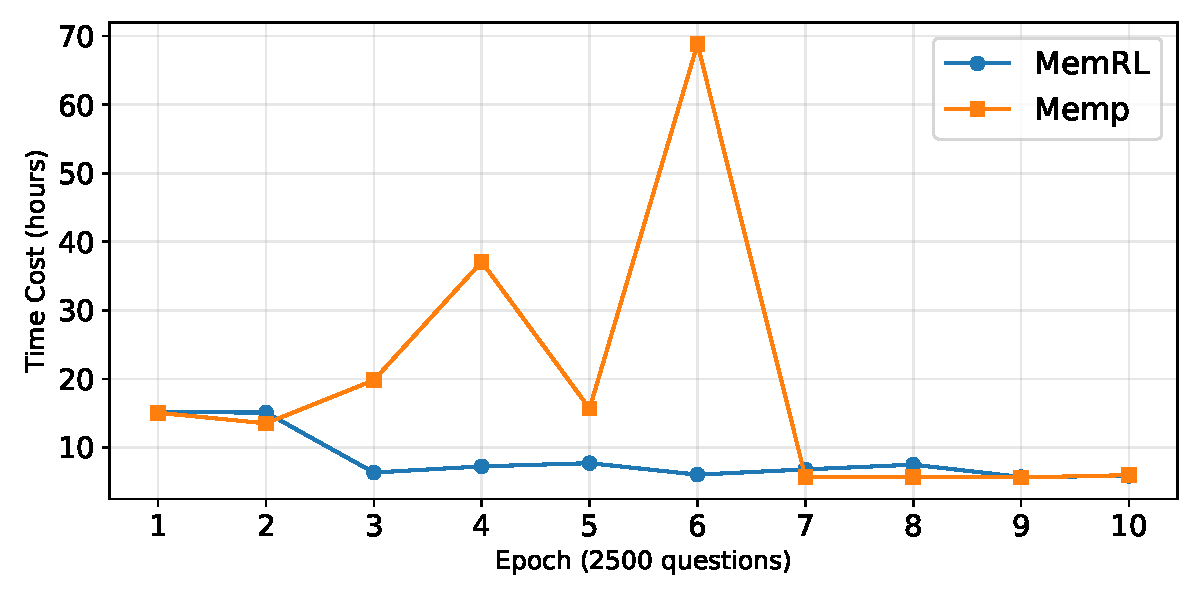
\includegraphics[width=0.5\linewidth]{latency_comparison_static.pdf}
    \caption{\textbf{Wall-Clock Time per Epoch on HLE.} The x-axis represents learning epochs (2,500 questions per epoch), and the y-axis represents the total time in hours. \textsc{MemRL} exhibits a stable runtime profile, confirming that the algorithmic overhead is negligible compared to system variances (e.g., network latency).}
    \label{fig:time_cost}
\end{figure}

\paragraph{Negligible Algorithmic Overhead.}
Figure~\ref{fig:time_cost} demonstrates that the runtime of \textsc{MemRL} is commensurate with, and often more stable than, that of MemP. The fluctuations observed (e.g., the spikes in the MemP curve at Epochs 4 and 6) are attributed to external factors such as API network latency and throughput variability, rather than algorithmic complexity.

Specifically, the additional components in \textsc{MemRL} introduce minimal computational cost:
\begin{itemize}
    \item \textbf{Dual-Stage Retrieval:} This involves basic vector dot-products and scalar score weighting, operating in milliseconds.
    \item \textbf{RL Update:} The Q-value update in a Monte Carlo style on scalars, which is an $O(1)$ operation.
\end{itemize}

Compared to the hours required for LLM generation over 2,500 questions, these millisecond-level operations are virtually imperceptible. The stability of the \textsc{MemRL} curve further suggests that our method does not introduce complex blocking operations that would exacerbate network-induced delays.


\section{Extended Limitations and Future Work}\label{app:future_work}

This appendix provides a more detailed discussion on the limitations of \textsc{MemRL} and outlines promising avenues for future research, building upon the foundations established in the main paper.

\subsection{Update Protocols and Memory Consolidation}
The current step-wise update protocol of \textsc{MemRL}, while enabling rapid adaptation, can introduce high-variance noise in long-horizon trajectories. This presents a challenge for stabilizing value estimation over extended sequences. A valuable future direction involves exploring more robust multi-step update mechanisms, which could offer slower but more stable learning. Furthermore, combining these with periodic consolidation of similar intentions and experiences within the memory bank could significantly improve the spatial efficiency of the memory, reducing redundancy and enhancing retrieval quality.

\subsection{Precise Credit Assignment in Multi-Memory Updates}
A significant challenge arises from the credit-assignment ambiguity encountered when multiple experiences from the memory are referenced and updated simultaneously. Determining the precise contribution of each referenced memory to the final outcome is complex and affects the efficiency of learning. Future research could investigate methods for more precise experience attribution, drawing inspiration from techniques like Shapley values~\citep{shapley1953value}, commonly used in cooperative game theory, or value decomposition methods prevalent in multi-agent reinforcement learning~\citep{rashid2020monotonic,sunehag2017value}. Such approaches could lead to more accurate updates and faster convergence.

\subsection{Task Similarity and Generalization}
\textsc{MemRL}'s effectiveness is observed to improve with the number of encountered tasks, aligning well with the characteristics of runtime learning. This is because the algorithm leverages past experiences, and a richer, more diverse set of similar experiences directly enhances its ability to retrieve relevant knowledge. However, when task similarity in the experience base is low, the method may inherently degrade into a less efficient reflection-like behavior, as direct experience transfer is limited. This is not a deficiency of the method but rather a characteristic of its reliance on learned utility from memory. For industrial deployment and real-world applications, this implies that maintaining a sufficiently high ``task similarity density" within the agent's operating environment or its collected memory is crucial. Strategies to achieve this could include active curriculum learning, environment design that promotes diverse yet related tasks, or techniques that facilitate hierarchical abstraction to enable generalization beyond direct, low-level experience matches. Enhancing retrieval mechanisms to proactively identify and adapt to novel task structures, or integrating hierarchical abstraction, are key for improving cross-task generalization.

\subsection{Memory Security and Robustness to Attack}
\textsc{MemRL} is sensitive to the quality of feedback, particularly vulnerable to ``reward hacking" if the verifier produces false positives. Incorrectly learned high Q-values from spurious feedback can quickly solidify and propagate erroneous behavioral patterns, leading to systemic failures. This highlights a critical challenge: memory security. A maliciously injected sample into the memory bank could rapidly diffuse pollution, potentially causing an intelligent agent to collapse. Future research must address the safety and trustworthiness of agent memories. Fortunately, the mutable nature of experience offers a silver lining: once contamination or attack is identified, polluted experiences can be swiftly pruned, allowing for recovery without disrupting the utility of previously learned valid experiences.

\subsection{Multi-Agent Collaboration and Shared Memory}
As many enterprises transition from single agents to multi-agent clusters (swarms), the question of ``shared memory" becomes important. Does the \textsc{MemRL} approach support knowledge sharing, allowing lessons learned and updated Q-values from one agent to immediately benefit others? We've explored scenarios where the memory, treated as a persistent resource, can indeed be shared among different models or agents (Appendix~\ref{app:memory_transfer}). Furthermore, adopting a multi-agent paradigm, akin to distributed parameter updates, could be highly beneficial. Each agent could accumulate experience and save it as memory during its operation, contributing to a large, collective memory pool. This would enable different agents to implicitly leverage each other's learned experiences, fostering a more collaborative and efficient learning ecosystem.

Beyond this collective pooling, a significant and promising frontier involves investigating the selective nature of such knowledge diffusion through the lens of transfer learning. As the number of agents increases, particularly beyond simple pairings, the challenge of "what to share" and "with whom to share" becomes a critical research direction. Future work could explore mechanisms that differentiate between universally applicable procedural insights and task-specific noise, ensuring that memory transfer remains contextually relevant and avoids the risks of negative transfer. Navigating these trade-offs between global collective intelligence and targeted knowledge distribution will be essential for building scalable, self-evolving swarms.
\subsection{Dedicated Domains and Hybrid Architectures}
While this work strongly advocates for freezing large language models (LLMs) to prevent catastrophic forgetting, a question arises regarding highly specialized domains where the base model may not comprehend foundational terminology. Is \textsc{MemRL} alone sufficient in such cases? We anticipate a future hybrid model where companies periodically fine-tune foundational models (e.g., annually) to update their core vocabulary and understanding, while simultaneously leveraging \textsc{MemRL} for daily behavioral adaptation and runtime learning. This approach requires the base model to possess a relatively high level of ``intelligence" to initially grasp and subsequently learn new terms through interaction and feedback.


\section{Case Study: High-Utility Failure Analysis (Near-Misses)}
\label{app:case}
This appendix section provides qualitative case studies of high-value near-miss memories mined from the 10-epoch OS-Interaction run.
CS denotes \emph{Case Study}. Each box below contains: origin task, retrieved reflection memory, a short explanation, and the target task where it was retrieved.

% Style
\tcbset{boxsep=1.0mm}
\newtcolorbox{CaseBox}[1]{%
  enhanced,
  breakable,
  colback=white,
  colframe=black!55,
  colbacktitle=black!6,
  coltitle=black,
  fonttitle=\bfseries,
  title={#1},
  boxrule=0.5pt,
  arc=2pt,
  left=6pt,right=6pt,top=6pt,bottom=6pt,
}
\newtcblisting{CodeBox}{%
  listing engine=listings,
  listing only,
  breakable,
  colback=black!1,
  colframe=black!35,
  boxrule=0.4pt,
  arc=2pt,
  left=6pt,right=6pt,top=4pt,bottom=4pt,
  listing options={
    basicstyle=\ttfamily\small,
    columns=fullflexible,
    keepspaces=true,
    breaklines=true,
    breakatwhitespace=false,
    showstringspaces=false
  },
}

\begin{CaseBox}{Case Study 1 (CS1)}
\textbf{Utility.} selected=19, success=19 (100.0\%).
\par\medskip
\textbf{Origin task.}
\begin{CodeBox}
Update the SSH daemon configuration using sed to set: Port=2222, PermitRootLogin=no, X11Forwarding=no, ClientAliveInterval=300, ClientAliveCountMax=2, MaxAuthTries=2, MaxSessions=2, PasswordAuthentication=no, AllowUsers='user1 user2', UseDNS=no, and Protocol=2.
\end{CodeBox}
\medskip
\textbf{Retrieved reflection memory.}
\begin{CodeBox}
- #1: [MEMORY TYPE] FAILURE_REFLECTION
[TASK]
Update the SSH daemon configuration using sed to set: Port=2222, PermitRootLogin=no, X11Forwarding=no, ClientAliveInterval=300, ClientAliveCountMax=2, MaxAuthTries=2, MaxSessions=2, PasswordAuthentication=no, AllowUsers='user1 user2', UseDNS=no, and Protocol=2.

[REFLECTION]
- ROOT CAUSE: The `sed` command did not modify the commented lines in the configuration file, which is why the new settings were not applied as expected.
- PATTERN TO AVOID: Avoid assuming that `sed` will replace commented lines without explicitly handling them.
- CORRECT APPROACH: Use `sed` to either uncomment the lines before replacing them or add the new configurations if they are commented out.
\end{CodeBox}
\par\medskip
\textbf{Explanation.} This reflection captures a subtle config-edit pitfall: naive sed replacement may miss commented defaults. The transferable lesson is to explicitly handle commented lines (uncomment-or-append), which generalizes across configuration-editing tasks.
\par\medskip
\textbf{Target task} (retrieval rank 1; run outcome: correct).
\begin{CodeBox}
Modify the SSH daemon configuration file at /etc/ssh/sshd_config to change the port to 2222, disable root login, set max sessions to 2, and set client alive interval to 300. Create a backup file before making changes.
\end{CodeBox}
\end{CaseBox}
\medskip

\begin{CaseBox}{Case Study 2 (CS2)}
\textbf{Utility.} selected=20, success=20 (100.0\%).
\par\medskip
\textbf{Origin task.}
\begin{CodeBox}
Replace 'DEBUG=True' with 'DEBUG=False' in /app/settings.cfg, append 'LOG_LEVEL=INFO' after the modified line, and create a backup file.
\end{CodeBox}
\medskip
\textbf{Retrieved reflection memory.}
\begin{CodeBox}
- #2: [MEMORY TYPE] FAILURE_REFLECTION
[TASK]
Replace 'DEBUG=True' with 'DEBUG=False' in /app/settings.cfg, append 'LOG_LEVEL=INFO' after the modified line, and create a backup file.

[REFLECTION]
- ROOT CAUSE: The `sed` command added the line `LOG_LEVEL=INFO` twice due to the way it was structured to append after the modified `DEBUG` line. 
- PATTERN TO AVOID: Avoid using multiple `-e` options in `sed` that can lead to unintended duplications when appending lines.
- CORRECT APPROACH: Instead, use a single `sed` command that ensures the line is only added once, or check for the existence of the line before appending it.
\end{CodeBox}
\par\medskip
\textbf{Explanation.} The originating attempt nearly completes the edit but fails due to a non-idempotent text transformation (duplicating an appended line). The memory teaches an idempotent editing pattern (single-pass edit or existence check), which transfers to many file-edit tasks.
\par\medskip
\textbf{Target task} (retrieval rank 2; run outcome: correct).
\begin{CodeBox}
Replace 'DEBUG=True' with 'DEBUG=False' in /app/settings.cfg, append 'LOG_LEVEL=INFO' after the modified line, and create a backup file.
\end{CodeBox}
\end{CaseBox}
\medskip

\begin{CaseBox}{Case Study 3 (CS3)}
\textbf{Utility.} selected=48, success=44 (91.7\%).
\par\medskip
\textbf{Origin task.}
\begin{CodeBox}
Create a user 'testuser' with a home directory, set password expiration policy (max 60 days, min 7 days, warning 7 days), add to 'testgroup', create '/home/testuser/private' with 770 permissions, create '/shared' directory accessible only by 'testgroup', add 'export PATH=$PATH:/custom' to .bashrc, and create '.hushlogin' file with 644 permissions.
\end{CodeBox}
\medskip
\textbf{Retrieved reflection memory.}
\begin{CodeBox}
- #4: [MEMORY TYPE] FAILURE_REFLECTION
[TASK]
Create a user 'testuser' with a home directory, set password expiration policy (max 60 days, min 7 days, warning 7 days), add to 'testgroup', create '/home/testuser/private' with 770 permissions, create '/shared' directory accessible only by 'testgroup', add 'export PATH=$PATH:/custom' to .bashrc, and create '.hushlogin' file with 644 permissions.

[REFLECTION]
- ROOT CAUSE: The output of the commands was empty, indicating successful execution without any visible confirmation or errors. 
- PATTERN TO AVOID: Relying solely on silent execution without feedback can lead to uncertainty about whether tasks were completed successfully. 
- CORRECT APPROACH: Always check the status of commands using conditional statements or output messages to confirm successful execution and provide clarity on the task's completion.
\end{CodeBox}
\par\medskip
\textbf{Explanation.} This memory highlights a common near-miss failure mode: assuming silent command output implies completion without verification. The transferable practice is to add explicit post-checks (exit codes, file/permission/ownership checks) after critical steps.
\par\medskip
\textbf{Target task} (retrieval rank 4; run outcome: correct).
\begin{CodeBox}
Create a user 'testuser' with a home directory, set password expiration policy (max 60 days, min 7 days, warning 7 days), add to 'testgroup', create '/home/testuser/private' with 770 permissions, create '/shared' directory accessible only by 'testgroup', add 'export PATH=$PATH:/custom' to .bashrc, and create '.hushlogin' file with 644 permissions.
\end{CodeBox}
\end{CaseBox}
\medskip

\begin{CaseBox}{Case Study 4 (CS4)}
\textbf{Utility.} selected=26, success=23 (88.5\%).
\par\medskip
\textbf{Origin task.}
\begin{CodeBox}
Run a sleep process in the background for 3 seconds, log its start and end times (in epoch format) to '/var/log/sleep.log', store the process ID in '/tmp/sleep_pid', and ensure the PID file is removed after the process completes.
\end{CodeBox}
\medskip
\textbf{Retrieved reflection memory.}
\begin{CodeBox}
- #1: [MEMORY TYPE] FAILURE_REFLECTION
[TASK]
Run a sleep process in the background for 3 seconds, log its start and end times (in epoch format) to '/var/log/sleep.log', store the process ID in '/tmp/sleep_pid', and ensure the PID file is removed after the process completes.

[REFLECTION]
- ROOT CAUSE: The PID file was not created because the command to capture the PID may not have executed correctly, leading to multiple executions of the sleep process without proper PID storage.
- PATTERN TO AVOID: Avoid executing commands in a loop or without proper checks, which can lead to unintended repeated executions and failures to capture necessary outputs.
- CORRECT APPROACH: Implement a structured approach with error handling and verification after each critical command to ensure that each step completes successfully before proceeding to the next.
\end{CodeBox}
\par\medskip
\textbf{Explanation.} The failure comes from missing control/verification around process management (PID capture and cleanup), which leads to repeated execution and missing artifacts. The memory transfers as a general recipe: capture PID once, verify artifacts, and sequence commands with error handling.
\par\medskip
\textbf{Target task} (retrieval rank 1; run outcome: correct).
\begin{CodeBox}
Run a sleep process in the background for 3 seconds, log its start and end times (in epoch format) to '/var/log/sleep.log', store the process ID in '/tmp/sleep_pid', and ensure the PID file is removed after the process completes.
\end{CodeBox}
\end{CaseBox}
\medskip

\begin{CaseBox}{Case Study 5 (CS5)}
\textbf{Utility.} selected=94, success=88 (93.6\%).
\par\medskip
\textbf{Origin task.}
\begin{CodeBox}
Create a secure configuration file '/etc/appconfig/settings.conf' using vi, set ownership to root:configgroup, permissions to 660, and add 'appuser' to 'configgroup'. Ensure the file contains '# Configuration file' and 'key=value' lines.
\end{CodeBox}
\medskip
\textbf{Retrieved reflection memory.}
\begin{CodeBox}
- #2: [MEMORY TYPE] FAILURE_REFLECTION
[TASK]
Create a secure configuration file '/etc/appconfig/settings.conf' using vi, set ownership to root:configgroup, permissions to 660, and add 'appuser' to 'configgroup'. Ensure the file contains '# Configuration file' and 'key=value' lines.

[REFLECTION]
- ROOT CAUSE: The initial assumption that the group `configgroup` and the user `appuser` already existed led to errors when attempting to set ownership and modify group membership.
- PATTERN TO AVOID: Avoid making assumptions about the existence of users or groups in the system without verifying first.
- CORRECT APPROACH: Always check for the existence of necessary users and groups before performing operations that depend on them, and create them if they do not exist.
\end{CodeBox}
\par\medskip
\textbf{Explanation.} This reflection encodes a high-frequency near-miss: assuming required users/groups exist. The transferable heuristic is to preflight environment state (e.g., id/getent) and create prerequisites before applying ownership/permission changes.
\par\medskip
\textbf{Target task} (retrieval rank 2; run outcome: correct).
\begin{CodeBox}
Create a configuration file '/etc/appconfig/settings.conf' using 'vi' containing the lines 'SERVER_IP=192.168.1.100' and 'DEBUG_MODE=false', set its group ownership to 'appgroup', and permissions to 640.
\end{CodeBox}
\end{CaseBox}
\medskip

\begin{CaseBox}{Case Study 6 (CS6)}
\textbf{Utility.} selected=59, success=55 (93.2\%).
\par\medskip
\textbf{Origin task.}
\begin{CodeBox}
Create a user 'testuser', add them to group 'testgroup', configure '/data' with group ownership 'testgroup' and permissions 770, create '/data/notes.txt' using 'vi' with content 'Hello from vi', and create an executable script '/check.sh' using 'vi' to verify group ownership of '/data'.
\end{CodeBox}
\medskip
\textbf{Retrieved reflection memory.}
\begin{CodeBox}
- #5: [MEMORY TYPE] FAILURE_REFLECTION
[TASK]
Create a user 'testuser', add them to group 'testgroup', configure '/data' with group ownership 'testgroup' and permissions 770, create '/data/notes.txt' using 'vi' with content 'Hello from vi', and create an executable script '/check.sh' using 'vi' to verify group ownership of '/data'.

[REFLECTION]
- ROOT CAUSE: The output being empty does not indicate a failure, but rather that the commands executed successfully without any output. 
- PATTERN TO AVOID: Assuming that an empty output signifies an error can lead to misunderstandings about command execution results. 
- CORRECT APPROACH: Always verify the success of commands by checking their exit status or using logging to confirm that actions were completed as intended.
\end{CodeBox}
\par\medskip
\textbf{Explanation.} The lesson is that empty output usually signals success, not failure; therefore success should be validated via exit status and direct state checks. This reduces false negatives across shell automation tasks.
\par\medskip
\textbf{Target task} (retrieval rank 5; run outcome: correct).
\begin{CodeBox}
Create a file '/shared/config/settings.conf' containing 'USER=testuser' and 'GROUP=testgroup', then programmatically create a user and group using the values from the file. Finally, ensure '/shared/data' is owned by the group with 770 permissions.
\end{CodeBox}
\end{CaseBox}
\medskip

% ==========================================
% Appendix G: Prompts
% ==========================================
\section{Prompts}
\label{app:prompts}
We provide the exact prompt strings and message templates used by our \textsc{MemRL} implementation 
across all benchmarks. To minimize ambiguity, we separate prompts used to summarize experiences into memories from
prompts used at task time for generation/inference.

% --- Box styles (aligned to the referenced case-study style) ---
\tcbset{boxsep=1.0mm}
\newtcolorbox{PromptBox}[1]{%
  enhanced,
  breakable,
  colback=white,
  colframe=black!55,
  colbacktitle=black!6,
  coltitle=black,
  fonttitle=\bfseries,
  title={#1},
  boxrule=0.5pt,
  arc=2pt,
  left=6pt,right=6pt,top=6pt,bottom=6pt,
}
\newtcblisting{PromptCode}{%
  listing engine=listings,
  listing only,
  breakable,
  colback=black!1,
  colframe=black!35,
  boxrule=0.4pt,
  arc=2pt,
  left=6pt,right=6pt,top=4pt,bottom=4pt,
  listing options={
    basicstyle=\ttfamily\small,
    columns=fullflexible,
    keepspaces=true,
    breaklines=true,
    breakatwhitespace=false,
    showstringspaces=false
  },
}

\subsection{Experience Summarization Prompts}
\label{app:memrl-prompts:experience-summarization}

\begin{PromptBox}{HLE: Experience Summarization Prompts}
\textbf{Trajectory serialization (stored as the episode trajectory).}
\begin{PromptCode}
QUESTION
{question}

SOLUTION
{model_output_stripped}
\end{PromptCode}
\medskip
\textbf{High-level script generation prompt.}
\begin{PromptCode}
Analyze the following detailed task trajectory and create a concise,
high-level script that captures the essential steps and decision points.

The script should be:
1. Generic enough to apply to similar tasks
2. Specific enough to provide useful guidance
3. 3-5 high-level steps maximum
4. Focus on the strategy and key decisions, not detailed actions

Trajectory:
{trajectory}

High-level script:
\end{PromptCode}
\medskip
\textbf{Failure reflection prompt.}
\begin{PromptCode}
Task: {task_description}

Failed trajectory:
{failed_trajectory}

This task failed. Analyze what went wrong and suggest improvements for future similar tasks.
Focus on:
1. Incorrect assumptions
2. Steps to improve
3. What to avoid next time

Provide a brief reflection:
\end{PromptCode}
\medskip
\textbf{Stored memory content templates.}
\begin{PromptCode}
# Successful memory
Task: {task_description}

SCRIPT:
{script}

TRAJECTORY:
{trajectory}

# Failure memory
TASK REFLECTION:
Task: {task_description}

What went wrong:
{reflection}

Failed approach:
{failed_trajectory}
\end{PromptCode}
\end{PromptBox}
\medskip

\begin{PromptBox}{ALFWorld: Experience Summarization Prompts}
\textbf{Trajectory serialization (stored as the episode trajectory).}
\begin{PromptCode}
The full ALFWorld dialogue history is stored as the trajectory:
  List[{"role": ..., "content": ...}, ...]
When interpolated into the summarization prompts, it is treated as a string representation.
\end{PromptCode}
\medskip
\textbf{High-level script generation prompt.}
\begin{PromptCode}
Analyze the following detailed task trajectory and create a concise,
high-level script that captures the essential steps and decision points.

The script should be:
1. Generic enough to apply to similar tasks
2. Specific enough to provide useful guidance
3. 3-5 high-level steps maximum
4. Focus on the strategy and key decisions, not detailed actions

Trajectory:
{trajectory}

High-level script:
\end{PromptCode}
\medskip
\textbf{Failure reflection prompt.}
\begin{PromptCode}
Task: {task_description}

Failed trajectory:
{failed_trajectory}

This task failed. Analyze what went wrong and suggest improvements for future similar tasks.
Focus on:
1. Incorrect assumptions
2. Steps to improve
3. What to avoid next time

Provide a brief reflection:
\end{PromptCode}
\medskip
\textbf{Stored memory content templates.}
\begin{PromptCode}
# Successful memory
Task: {task_description}

SCRIPT:
{script}

TRAJECTORY:
{trajectory}

# Failure memory
TASK REFLECTION:
Task: {task_description}

What went wrong:
{reflection}

Failed approach:
{failed_trajectory}
\end{PromptCode}
\end{PromptBox}
\medskip

\begin{PromptBox}{BCB (BigCodeBench): Experience Summarization Prompts}
\textbf{Trajectory serialization (stored as the episode trajectory).}
\begin{PromptCode}
[BCB] epoch={epoch} phase={phase} task_id={task_id}
[PROMPT]
{bcb_task_prompt}
[GENERATED CODE]
```python
{model_code}
```
[EVAL]
{"status": "...", "error": "..."}
\end{PromptCode}
\medskip
\textbf{High-level script generation prompt.}
\begin{PromptCode}
Analyze the following detailed task trajectory and create a concise,
high-level script that captures the essential steps and decision points.

The script should be:
1. Generic enough to apply to similar tasks
2. Specific enough to provide useful guidance
3. 3-5 high-level steps maximum
4. Focus on the strategy and key decisions, not detailed actions

Trajectory:
{trajectory}

High-level script:
\end{PromptCode}
\medskip
\textbf{Failure reflection prompt.}
\begin{PromptCode}
Task: {task_description}

Failed trajectory:
{failed_trajectory}

This task failed. Analyze what went wrong and suggest improvements for future similar tasks.
Focus on:
1. Incorrect assumptions
2. Steps to improve
3. What to avoid next time

Provide a brief reflection:
\end{PromptCode}
\medskip
\textbf{Stored memory content templates.}
\begin{PromptCode}
# Successful memory
Task: {task_description}

SCRIPT:
{script}

TRAJECTORY:
{trajectory}

# Failure memory
TASK REFLECTION:
Task: {task_description}

What went wrong:
{reflection}

Failed approach:
{failed_trajectory}
\end{PromptCode}
\end{PromptBox}
\medskip

\begin{PromptBox}{LLB (LifelongAgentBench): Experience Summarization Prompts}
\textbf{Trajectory serialization (stored as the episode trajectory).}
\begin{PromptCode}
{role_1}: {content_1}
{role_2}: {content_2}
...
\end{PromptCode}
\medskip
\textbf{High-level script generation prompt.}
\begin{PromptCode}
Analyze the following detailed task trajectory and create a concise,
high-level script that captures the essential steps and decision points.

The script should be:
1. Generic enough to apply to similar tasks
2. Specific enough to provide useful guidance
3. 3-5 high-level steps maximum
4. Focus on the strategy and key decisions, not detailed actions

Trajectory:
{trajectory}

High-level script:
\end{PromptCode}
\medskip
\textbf{Failure reflection prompt.}
\begin{PromptCode}
Task: {task_description}

Failed trajectory:
{failed_trajectory}

This task failed. Analyze what went wrong and suggest improvements for future similar tasks.
Focus on:
1. Incorrect assumptions
2. Steps to improve
3. What to avoid next time

Provide a brief reflection:
\end{PromptCode}
\medskip
\textbf{Stored memory content templates.}
\begin{PromptCode}
# Successful memory
Task: {task_description}

SCRIPT:
{script}

TRAJECTORY:
{trajectory}

# Failure memory
TASK REFLECTION:
Task: {task_description}

What went wrong:
{reflection}

Failed approach:
{failed_trajectory}
\end{PromptCode}
\end{PromptBox}
\medskip

\subsection{Generation and Inference Prompts}
\label{app:memrl-prompts:generation-inference}

\begin{PromptBox}{HLE: Generation and Inference Prompts}
\textbf{System prompt (exact-match).}
\begin{PromptCode}
Your response should be in the following format:
Explanation: {your explanation for your final answer}
Exact Answer: {your succinct, final answer}
Confidence: {your confidence score between 0% and 100% for your answer}
\end{PromptCode}
\medskip
\textbf{System prompt (multiple-choice).}
\begin{PromptCode}
Your response should be in the following format:
Explanation: {your explanation for your answer choice}
Answer: {your chosen answer}
Confidence: {your confidence score between 0% and 100% for your answer}
\end{PromptCode}
\medskip
\textbf{Retrieved memory injection (system message).}
\begin{PromptCode}
=== Successful Memories ===
{memory_full_content_1}

{memory_full_content_2}

=== Failed Memories (for caution) ===
{memory_full_content_3}
...
\end{PromptCode}
\medskip
\textbf{Optional repeat-attempt reflection note (system message).}
\begin{PromptCode}
You attempted this question before.
Result: {CORRECT|INCORRECT}
Question: {question}
Previous attempt (solution only):
{solution_only}
Reflect on mistakes or gaps, then solve the problem again with a better solution.
\end{PromptCode}
\medskip
\textbf{User message text block (when images exist).}
\begin{PromptCode}
Now solve the following question:

[Image IDs: {question_image_ids}]
{question}

Attached images:
1. [{img_id_1}] ({source_1})
2. [{img_id_2}] ({source_2})
...
\end{PromptCode}
\medskip
\textbf{Message ordering.}
\begin{PromptCode}
1) system: exact-match OR multiple-choice format prompt
2) system: optional reflection note (if enabled)
3) system: optional retrieved memory context
4) user: question content (text + optional images)
\end{PromptCode}
\end{PromptBox}
\medskip

\begin{PromptBox}{ALFWorld: Generation and Inference Prompts}
\textbf{Base system prompt (ReAct format + action space).}
\begin{PromptCode}
Interact with a household to solve a task. Imagine you are an intelligent agent in a household environment and your target is to perform actions to complete the task goal. At the beginning of your interactions, you will be given the detailed description of the current environment and your goal to accomplish.
For each of your turn, you will be given the observation of the last turn. You should first think about the current condition and plan for your future actions, and then output your action in this turn. Your output must strictly follow this format:"Thought: your thoughts.\nAction: your next action".

The available actions are:
1. go to {recep}
2. take {obj} from {recep}
3. move {obj} to {recep}
4. open {recep}
5. close {recep}
6. use {obj}
7. clean {obj} with {recep}
8. heat {obj} with {recep}
9. cool {obj} with {recep}
where {obj} and {recep} correspond to objects and receptacles.
After your each turn, the environment will give you immediate feedback based on which you plan your next few steps. if the envrionment output "Nothing happened", that means the previous action is invalid and you should try more options.

Your response should use the following format:

Thought: <your thoughts>
Action: <your next action>
\end{PromptCode}
\medskip
\textbf{Retrieved memory injection (system message).}
\begin{PromptCode}
In addition to the example, you have the following memories from your own past experiences. Use them to help you if they are relevant:

--- SUCCESSFUL MEMORIES (Examples to follow) ---
{formatted_success_memories_joined}

--- FAILED MEMORIES (Examples to avoid or learn from) ---
{formatted_failed_memories_joined}
\end{PromptCode}
\medskip
\textbf{Current task prompt (user message).}
\begin{PromptCode}
Now, it's your turn to solve a new task.
{task_description}
\end{PromptCode}
\medskip
\textbf{Per-step observation prompt (user message).}
\begin{PromptCode}
Observation: {observation}
\end{PromptCode}
\medskip
\textbf{Message ordering (high level).}
\begin{PromptCode}
1) system: base ALFWorld system prompt
2) user/assistant: selected few-shot example dialogue (sequence of messages)
3) system: optional retrieved memory context
4) user: new task prompt
5) loop: append user Observation: ..., model replies with Thought/Action
\end{PromptCode}
\end{PromptBox}
\medskip

\begin{PromptBox}{BCB (BigCodeBench): Generation and Inference Prompts}
\textbf{Retrieved memory injection (system message).}
\begin{PromptCode}
[Retrieved Memory Context]

### Memory 1 (id={mem_id_1}, sim={similarity_1})
{memory_content_1}

### Memory 2 (id={mem_id_2}, sim={similarity_2})
{memory_content_2}
...
\end{PromptCode}
\medskip
\textbf{Dataset-provided task prompt selection (user message).}
\begin{PromptCode}
if split == "instruct":
    return task["instruct_prompt"]
if split == "complete":
    return task["complete_prompt"]
\end{PromptCode}
\medskip
\textbf{Message ordering.}
\begin{PromptCode}
1) system: optional [Retrieved Memory Context] ...
2) user: {bcb_task_prompt}
\end{PromptCode}
\end{PromptBox}
\medskip

\begin{PromptBox}{LLB (LifelongAgentBench): Generation and Inference Prompts}
\textbf{Base system prompt.}
\begin{PromptCode}
You are an execution-focused AI agent solving database and operating-system tasks.

You may receive a [Retrieved Memory Context] block with past experiences from similar problems.
These are **references for learning**, not guaranteed solutions:
- [MEMORY TYPE] SUCCESS_PROCEDURE: A successful approach from a similar task learn the pattern.
- [MEMORY TYPE] FAILURE_REFLECTION: A failed attempt with lessons avoid similar mistakes.

Use the memories as inspiration, but always analyze your current task independently and
adapt your approach based on its specific requirements.
\end{PromptCode}
\medskip
\textbf{Strict output constraint (DB tasks).}
\begin{PromptCode}
STRICT OUTPUT FORMAT (LLB:DB, do not violate):
1) After your reasoning, include exactly ONE action line:
   - Action: Operation
   - Action: Answer
2) If Action: Operation, put exactly ONE SQL statement in the FIRST fenced code block using ```sql, on a single line. Do not add any extra text after that block.
3) If Action: Answer, include `Final Answer: ...` on the next line and do not add extra text after that.
\end{PromptCode}
\medskip
\textbf{Strict output constraint (OS tasks).}
\begin{PromptCode}
STRICT OUTPUT FORMAT (LLB:OS, do not violate):
1) After your reasoning, include exactly ONE action line:
   - Act: bash
   - Act: finish
2) If Act: bash, the next lines MUST be a ```bash fenced code block with your Bash commands. Do not include any other code blocks.
3) If Act: finish, it must be the last line (no code blocks, no extra text).
4) Do NOT use `Action:` in OS tasks (use `Act:` only).
\end{PromptCode}
\medskip
\textbf{Retrieved memory injection block.}
\begin{PromptCode}
[Retrieved Memory Context]

=== SUCCESSFUL EXPERIENCES (Learn from these) ===
[SUCCESS 1] [TYPE: {mem_type}]
{content}

=== FAILED EXPERIENCES (Avoid these mistakes) ===
[FAILURE 1] [TYPE: {mem_type}]
{content}
\end{PromptCode}
\medskip
\textbf{Prompt assembly ordering (system prompt).}
\begin{PromptCode}
1) base system prompt
2) optional [Retrieved Memory Context] ...
3) strict output format block appended at the end (task-aligned)
\end{PromptCode}
\end{PromptBox}
\end{document}


